\documentclass[twoside]{book}

% Packages required by doxygen
\usepackage{fixltx2e}
\usepackage{calc}
\usepackage{doxygen}
\usepackage[export]{adjustbox} % also loads graphicx
\usepackage{graphicx}
\usepackage[utf8]{inputenc}
\usepackage{makeidx}
\usepackage{multicol}
\usepackage{multirow}
\PassOptionsToPackage{warn}{textcomp}
\usepackage{textcomp}
\usepackage[nointegrals]{wasysym}
\usepackage[table]{xcolor}

% Font selection
\usepackage[T1]{fontenc}
\usepackage[scaled=.90]{helvet}
\usepackage{courier}
\usepackage{amssymb}
\usepackage{sectsty}
\renewcommand{\familydefault}{\sfdefault}
\allsectionsfont{%
  \fontseries{bc}\selectfont%
  \color{darkgray}%
}
\renewcommand{\DoxyLabelFont}{%
  \fontseries{bc}\selectfont%
  \color{darkgray}%
}
\newcommand{\+}{\discretionary{\mbox{\scriptsize$\hookleftarrow$}}{}{}}

% Page & text layout
\usepackage{geometry}
\geometry{%
  a4paper,%
  top=2.5cm,%
  bottom=2.5cm,%
  left=2.5cm,%
  right=2.5cm%
}
\tolerance=750
\hfuzz=15pt
\hbadness=750
\setlength{\emergencystretch}{15pt}
\setlength{\parindent}{0cm}
\setlength{\parskip}{3ex plus 2ex minus 2ex}
\makeatletter
\renewcommand{\paragraph}{%
  \@startsection{paragraph}{4}{0ex}{-1.0ex}{1.0ex}{%
    \normalfont\normalsize\bfseries\SS@parafont%
  }%
}
\renewcommand{\subparagraph}{%
  \@startsection{subparagraph}{5}{0ex}{-1.0ex}{1.0ex}{%
    \normalfont\normalsize\bfseries\SS@subparafont%
  }%
}
\makeatother

% Headers & footers
\usepackage{fancyhdr}
\pagestyle{fancyplain}
\fancyhead[LE]{\fancyplain{}{\bfseries\thepage}}
\fancyhead[CE]{\fancyplain{}{}}
\fancyhead[RE]{\fancyplain{}{\bfseries\leftmark}}
\fancyhead[LO]{\fancyplain{}{\bfseries\rightmark}}
\fancyhead[CO]{\fancyplain{}{}}
\fancyhead[RO]{\fancyplain{}{\bfseries\thepage}}
\fancyfoot[LE]{\fancyplain{}{}}
\fancyfoot[CE]{\fancyplain{}{}}
\fancyfoot[RE]{\fancyplain{}{\bfseries\scriptsize Generated by Doxygen }}
\fancyfoot[LO]{\fancyplain{}{\bfseries\scriptsize Generated by Doxygen }}
\fancyfoot[CO]{\fancyplain{}{}}
\fancyfoot[RO]{\fancyplain{}{}}
\renewcommand{\footrulewidth}{0.4pt}
\renewcommand{\chaptermark}[1]{%
  \markboth{#1}{}%
}
\renewcommand{\sectionmark}[1]{%
  \markright{\thesection\ #1}%
}

% Indices & bibliography
\usepackage{natbib}
\usepackage[titles]{tocloft}
\setcounter{tocdepth}{3}
\setcounter{secnumdepth}{5}
\makeindex

% Hyperlinks (required, but should be loaded last)
\usepackage{ifpdf}
\ifpdf
  \usepackage[pdftex,pagebackref=true]{hyperref}
\else
  \usepackage[ps2pdf,pagebackref=true]{hyperref}
\fi
\hypersetup{%
  colorlinks=true,%
  linkcolor=blue,%
  citecolor=blue,%
  unicode%
}

% Custom commands
\newcommand{\clearemptydoublepage}{%
  \newpage{\pagestyle{empty}\cleardoublepage}%
}

\usepackage{caption}
\captionsetup{labelsep=space,justification=centering,font={bf},singlelinecheck=off,skip=4pt,position=top}

%===== C O N T E N T S =====

\begin{document}

% Titlepage & ToC
\hypersetup{pageanchor=false,
             bookmarksnumbered=true,
             pdfencoding=unicode
            }
\pagenumbering{alph}
\begin{titlepage}
\vspace*{7cm}
\begin{center}%
{\Large T\+M\+S\+E\+N\+G\+I\+NE }\\
\vspace*{1cm}
{\large Generated by Doxygen 1.8.14}\\
\end{center}
\end{titlepage}
\clearemptydoublepage
\pagenumbering{roman}
\tableofcontents
\clearemptydoublepage
\pagenumbering{arabic}
\hypersetup{pageanchor=true}

%--- Begin generated contents ---
\chapter{Namespace Index}
\section{Namespace List}
Here is a list of all namespaces with brief descriptions\+:\begin{DoxyCompactList}
\item\contentsline{section}{\hyperlink{namespacetmsengine}{tmsengine} }{\pageref{namespacetmsengine}}{}
\end{DoxyCompactList}

\chapter{Hierarchical Index}
\section{Class Hierarchy}
This inheritance list is sorted roughly, but not completely, alphabetically\+:\begin{DoxyCompactList}
\item \contentsline{section}{tmsengine\+:\+:Component}{\pageref{classtmsengine_1_1_component}}{}
\begin{DoxyCompactList}
\item \contentsline{section}{tmsengine\+:\+:Camera}{\pageref{classtmsengine_1_1_camera}}{}
\item \contentsline{section}{tmsengine\+:\+:Mesh\+Renderer}{\pageref{classtmsengine_1_1_mesh_renderer}}{}
\item \contentsline{section}{tmsengine\+:\+:Transform}{\pageref{classtmsengine_1_1_transform}}{}
\end{DoxyCompactList}
\item \contentsline{section}{tmsengine\+:\+:Core}{\pageref{classtmsengine_1_1_core}}{}
\item \contentsline{section}{tmsengine\+:\+:Enviroment}{\pageref{classtmsengine_1_1_enviroment}}{}
\item \contentsline{section}{tmsengine\+:\+:Game\+Object}{\pageref{classtmsengine_1_1_game_object}}{}
\item \contentsline{section}{tmsengine\+:\+:Keyboard}{\pageref{classtmsengine_1_1_keyboard}}{}
\item \contentsline{section}{Material}{\pageref{class_material}}{}
\item \contentsline{section}{Material\+Attribute}{\pageref{class_material_attribute}}{}
\item \contentsline{section}{Mesh}{\pageref{class_mesh}}{}
\item \contentsline{section}{Resource}{\pageref{class_resource}}{}
\item \contentsline{section}{Resources}{\pageref{class_resources}}{}
\item \contentsline{section}{tmsengine\+:\+:Sampler}{\pageref{structtmsengine_1_1_sampler}}{}
\item \contentsline{section}{tmsengine\+:\+:Screen}{\pageref{classtmsengine_1_1_screen}}{}
\item \contentsline{section}{Shader}{\pageref{class_shader}}{}
\item \contentsline{section}{tmsengine\+:\+:Shader\+Program}{\pageref{classtmsengine_1_1_shader_program}}{}
\item \contentsline{section}{tmsengine\+:\+:Sound}{\pageref{classtmsengine_1_1_sound}}{}
\item \contentsline{section}{tmsengine\+:\+:Sound\+Impl}{\pageref{structtmsengine_1_1_sound_impl}}{}
\item \contentsline{section}{tmsengine\+:\+:Texture}{\pageref{classtmsengine_1_1_texture}}{}
\item \contentsline{section}{Triangle}{\pageref{struct_triangle}}{}
\item \contentsline{section}{tmsengine\+:\+:Vertex\+Array}{\pageref{classtmsengine_1_1_vertex_array}}{}
\item \contentsline{section}{tmsengine\+:\+:Vertex\+Buffer}{\pageref{classtmsengine_1_1_vertex_buffer}}{}
\end{DoxyCompactList}

\chapter{Class Index}
\section{Class List}
Here are the classes, structs, unions and interfaces with brief descriptions\+:\begin{DoxyCompactList}
\item\contentsline{section}{\hyperlink{classtmsengine_1_1_camera}{tmsengine\+::\+Camera} }{\pageref{classtmsengine_1_1_camera}}{}
\item\contentsline{section}{\hyperlink{classtmsengine_1_1_component}{tmsengine\+::\+Component} }{\pageref{classtmsengine_1_1_component}}{}
\item\contentsline{section}{\hyperlink{classtmsengine_1_1_core}{tmsengine\+::\+Core} }{\pageref{classtmsengine_1_1_core}}{}
\item\contentsline{section}{\hyperlink{classtmsengine_1_1_enviroment}{tmsengine\+::\+Enviroment} }{\pageref{classtmsengine_1_1_enviroment}}{}
\item\contentsline{section}{\hyperlink{classtmsengine_1_1_game_object}{tmsengine\+::\+Game\+Object} }{\pageref{classtmsengine_1_1_game_object}}{}
\item\contentsline{section}{\hyperlink{classtmsengine_1_1_keyboard}{tmsengine\+::\+Keyboard} }{\pageref{classtmsengine_1_1_keyboard}}{}
\item\contentsline{section}{\hyperlink{class_material}{Material} }{\pageref{class_material}}{}
\item\contentsline{section}{\hyperlink{class_material_attribute}{Material\+Attribute} }{\pageref{class_material_attribute}}{}
\item\contentsline{section}{\hyperlink{class_mesh}{Mesh} }{\pageref{class_mesh}}{}
\item\contentsline{section}{\hyperlink{classtmsengine_1_1_mesh_renderer}{tmsengine\+::\+Mesh\+Renderer} }{\pageref{classtmsengine_1_1_mesh_renderer}}{}
\item\contentsline{section}{\hyperlink{class_resource}{Resource} }{\pageref{class_resource}}{}
\item\contentsline{section}{\hyperlink{class_resources}{Resources} }{\pageref{class_resources}}{}
\item\contentsline{section}{\hyperlink{structtmsengine_1_1_sampler}{tmsengine\+::\+Sampler} }{\pageref{structtmsengine_1_1_sampler}}{}
\item\contentsline{section}{\hyperlink{classtmsengine_1_1_screen}{tmsengine\+::\+Screen} }{\pageref{classtmsengine_1_1_screen}}{}
\item\contentsline{section}{\hyperlink{class_shader}{Shader} }{\pageref{class_shader}}{}
\item\contentsline{section}{\hyperlink{classtmsengine_1_1_shader_program}{tmsengine\+::\+Shader\+Program} }{\pageref{classtmsengine_1_1_shader_program}}{}
\item\contentsline{section}{\hyperlink{classtmsengine_1_1_sound}{tmsengine\+::\+Sound} }{\pageref{classtmsengine_1_1_sound}}{}
\item\contentsline{section}{\hyperlink{structtmsengine_1_1_sound_impl}{tmsengine\+::\+Sound\+Impl} }{\pageref{structtmsengine_1_1_sound_impl}}{}
\item\contentsline{section}{\hyperlink{classtmsengine_1_1_texture}{tmsengine\+::\+Texture} }{\pageref{classtmsengine_1_1_texture}}{}
\item\contentsline{section}{\hyperlink{classtmsengine_1_1_transform}{tmsengine\+::\+Transform} }{\pageref{classtmsengine_1_1_transform}}{}
\item\contentsline{section}{\hyperlink{struct_triangle}{Triangle} }{\pageref{struct_triangle}}{}
\item\contentsline{section}{\hyperlink{classtmsengine_1_1_vertex_array}{tmsengine\+::\+Vertex\+Array} }{\pageref{classtmsengine_1_1_vertex_array}}{}
\item\contentsline{section}{\hyperlink{classtmsengine_1_1_vertex_buffer}{tmsengine\+::\+Vertex\+Buffer} }{\pageref{classtmsengine_1_1_vertex_buffer}}{}
\end{DoxyCompactList}

\chapter{File Index}
\section{File List}
Here is a list of all files with brief descriptions\+:\begin{DoxyCompactList}
\item\contentsline{section}{T\+M\+S\+Engine/\hyperlink{_camera_8cpp}{Camera.\+cpp} }{\pageref{_camera_8cpp}}{}
\item\contentsline{section}{T\+M\+S\+Engine/\hyperlink{_camera_8h}{Camera.\+h} }{\pageref{_camera_8h}}{}
\item\contentsline{section}{T\+M\+S\+Engine/\hyperlink{_component_8cpp}{Component.\+cpp} }{\pageref{_component_8cpp}}{}
\item\contentsline{section}{T\+M\+S\+Engine/\hyperlink{_component_8h}{Component.\+h} }{\pageref{_component_8h}}{}
\item\contentsline{section}{T\+M\+S\+Engine/\hyperlink{_core_8cpp}{Core.\+cpp} }{\pageref{_core_8cpp}}{}
\item\contentsline{section}{T\+M\+S\+Engine/\hyperlink{_core_8h}{Core.\+h} }{\pageref{_core_8h}}{}
\item\contentsline{section}{T\+M\+S\+Engine/\hyperlink{_enviroment_8cpp}{Enviroment.\+cpp} }{\pageref{_enviroment_8cpp}}{}
\item\contentsline{section}{T\+M\+S\+Engine/\hyperlink{_enviroment_8h}{Enviroment.\+h} }{\pageref{_enviroment_8h}}{}
\item\contentsline{section}{T\+M\+S\+Engine/\hyperlink{_game_object_8cpp}{Game\+Object.\+cpp} }{\pageref{_game_object_8cpp}}{}
\item\contentsline{section}{T\+M\+S\+Engine/\hyperlink{_game_object_8h}{Game\+Object.\+h} }{\pageref{_game_object_8h}}{}
\item\contentsline{section}{T\+M\+S\+Engine/\hyperlink{_keyboard_8cpp}{Keyboard.\+cpp} }{\pageref{_keyboard_8cpp}}{}
\item\contentsline{section}{T\+M\+S\+Engine/\hyperlink{_keyboard_8h}{Keyboard.\+h} }{\pageref{_keyboard_8h}}{}
\item\contentsline{section}{T\+M\+S\+Engine/\hyperlink{_material_8cpp}{Material.\+cpp} }{\pageref{_material_8cpp}}{}
\item\contentsline{section}{T\+M\+S\+Engine/\hyperlink{_material_8h}{Material.\+h} }{\pageref{_material_8h}}{}
\item\contentsline{section}{T\+M\+S\+Engine/\hyperlink{_material_attribute_8cpp}{Material\+Attribute.\+cpp} }{\pageref{_material_attribute_8cpp}}{}
\item\contentsline{section}{T\+M\+S\+Engine/\hyperlink{_material_attribute_8h}{Material\+Attribute.\+h} }{\pageref{_material_attribute_8h}}{}
\item\contentsline{section}{T\+M\+S\+Engine/\hyperlink{_mesh_renderer_8cpp}{Mesh\+Renderer.\+cpp} }{\pageref{_mesh_renderer_8cpp}}{}
\item\contentsline{section}{T\+M\+S\+Engine/\hyperlink{_mesh_renderer_8h}{Mesh\+Renderer.\+h} }{\pageref{_mesh_renderer_8h}}{}
\item\contentsline{section}{T\+M\+S\+Engine/\hyperlink{_resource_manager_8cpp}{Resource\+Manager.\+cpp} }{\pageref{_resource_manager_8cpp}}{}
\item\contentsline{section}{T\+M\+S\+Engine/\hyperlink{_resource_manager_8h}{Resource\+Manager.\+h} }{\pageref{_resource_manager_8h}}{}
\item\contentsline{section}{T\+M\+S\+Engine/\hyperlink{_screen_8cpp}{Screen.\+cpp} }{\pageref{_screen_8cpp}}{}
\item\contentsline{section}{T\+M\+S\+Engine/\hyperlink{_screen_8h}{Screen.\+h} }{\pageref{_screen_8h}}{}
\item\contentsline{section}{T\+M\+S\+Engine/\hyperlink{_shader_program_8cpp}{Shader\+Program.\+cpp} }{\pageref{_shader_program_8cpp}}{}
\item\contentsline{section}{T\+M\+S\+Engine/\hyperlink{_shader_program_8h}{Shader\+Program.\+h} }{\pageref{_shader_program_8h}}{}
\item\contentsline{section}{T\+M\+S\+Engine/\hyperlink{_sound_8cpp}{Sound.\+cpp} }{\pageref{_sound_8cpp}}{}
\item\contentsline{section}{T\+M\+S\+Engine/\hyperlink{_sound_8h}{Sound.\+h} }{\pageref{_sound_8h}}{}
\item\contentsline{section}{T\+M\+S\+Engine/\hyperlink{_t_m_s_engine_8h}{T\+M\+S\+Engine.\+h} }{\pageref{_t_m_s_engine_8h}}{}
\item\contentsline{section}{T\+M\+S\+Engine/\hyperlink{_transform_8cpp}{Transform.\+cpp} }{\pageref{_transform_8cpp}}{}
\item\contentsline{section}{T\+M\+S\+Engine/\hyperlink{_transform_8h}{Transform.\+h} }{\pageref{_transform_8h}}{}
\item\contentsline{section}{T\+M\+S\+Engine/\hyperlink{_vertex_array_8cpp}{Vertex\+Array.\+cpp} }{\pageref{_vertex_array_8cpp}}{}
\item\contentsline{section}{T\+M\+S\+Engine/\hyperlink{_vertex_array_8h}{Vertex\+Array.\+h} }{\pageref{_vertex_array_8h}}{}
\item\contentsline{section}{T\+M\+S\+Engine/\hyperlink{_vertex_buffer_8cpp}{Vertex\+Buffer.\+cpp} }{\pageref{_vertex_buffer_8cpp}}{}
\item\contentsline{section}{T\+M\+S\+Engine/\hyperlink{_vertex_buffer_8h}{Vertex\+Buffer.\+h} }{\pageref{_vertex_buffer_8h}}{}
\item\contentsline{section}{T\+M\+S\+Engine/\+Resources/\hyperlink{_mesh_8cpp}{Mesh.\+cpp} }{\pageref{_mesh_8cpp}}{}
\item\contentsline{section}{T\+M\+S\+Engine/\+Resources/\hyperlink{_mesh_8h}{Mesh.\+h} }{\pageref{_mesh_8h}}{}
\item\contentsline{section}{T\+M\+S\+Engine/\+Resources/\hyperlink{_resource_8cpp}{Resource.\+cpp} }{\pageref{_resource_8cpp}}{}
\item\contentsline{section}{T\+M\+S\+Engine/\+Resources/\hyperlink{_resource_8h}{Resource.\+h} }{\pageref{_resource_8h}}{}
\item\contentsline{section}{T\+M\+S\+Engine/\+Resources/\hyperlink{_shader_8cpp}{Shader.\+cpp} }{\pageref{_shader_8cpp}}{}
\item\contentsline{section}{T\+M\+S\+Engine/\+Resources/\hyperlink{_shader_8h}{Shader.\+h} }{\pageref{_shader_8h}}{}
\item\contentsline{section}{T\+M\+S\+Engine/\+Resources/\hyperlink{_texture_8cpp}{Texture.\+cpp} }{\pageref{_texture_8cpp}}{}
\item\contentsline{section}{T\+M\+S\+Engine/\+Resources/\hyperlink{_texture_8h}{Texture.\+h} }{\pageref{_texture_8h}}{}
\end{DoxyCompactList}

\chapter{Namespace Documentation}
\hypertarget{namespacetmsengine}{}\section{tmsengine Namespace Reference}
\label{namespacetmsengine}\index{tmsengine@{tmsengine}}
\subsection*{Classes}
\begin{DoxyCompactItemize}
\item 
class \hyperlink{classtmsengine_1_1_camera}{Camera}
\item 
class \hyperlink{classtmsengine_1_1_component}{Component}
\item 
class \hyperlink{classtmsengine_1_1_core}{Core}
\item 
class \hyperlink{classtmsengine_1_1_enviroment}{Enviroment}
\item 
class \hyperlink{classtmsengine_1_1_game_object}{Game\+Object}
\item 
class \hyperlink{classtmsengine_1_1_keyboard}{Keyboard}
\item 
class \hyperlink{classtmsengine_1_1_mesh_renderer}{Mesh\+Renderer}
\item 
struct \hyperlink{structtmsengine_1_1_sampler}{Sampler}
\item 
class \hyperlink{classtmsengine_1_1_screen}{Screen}
\item 
class \hyperlink{classtmsengine_1_1_shader_program}{Shader\+Program}
\item 
class \hyperlink{classtmsengine_1_1_sound}{Sound}
\item 
struct \hyperlink{structtmsengine_1_1_sound_impl}{Sound\+Impl}
\item 
class \hyperlink{classtmsengine_1_1_texture}{Texture}
\item 
class \hyperlink{classtmsengine_1_1_transform}{Transform}
\item 
class \hyperlink{classtmsengine_1_1_vertex_array}{Vertex\+Array}
\item 
class \hyperlink{classtmsengine_1_1_vertex_buffer}{Vertex\+Buffer}
\end{DoxyCompactItemize}

\chapter{Class Documentation}
\hypertarget{classtmsengine_1_1_camera}{}\section{tmsengine\+:\+:Camera Class Reference}
\label{classtmsengine_1_1_camera}\index{tmsengine\+::\+Camera@{tmsengine\+::\+Camera}}


{\ttfamily \#include $<$Camera.\+h$>$}



Inheritance diagram for tmsengine\+:\+:Camera\+:\nopagebreak
\begin{figure}[H]
\begin{center}
\leavevmode
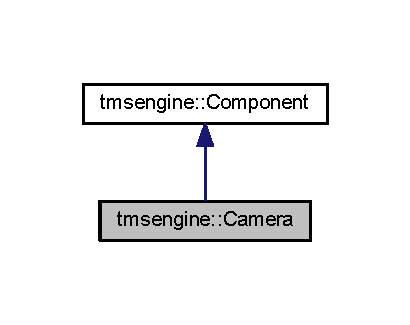
\includegraphics[width=197pt]{classtmsengine_1_1_camera__inherit__graph}
\end{center}
\end{figure}


Collaboration diagram for tmsengine\+:\+:Camera\+:\nopagebreak
\begin{figure}[H]
\begin{center}
\leavevmode
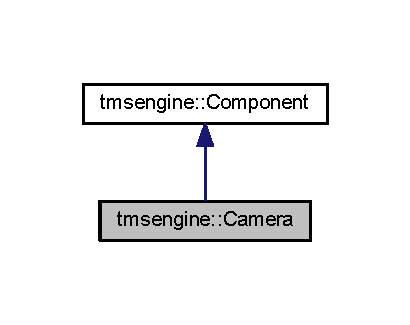
\includegraphics[width=197pt]{classtmsengine_1_1_camera__coll__graph}
\end{center}
\end{figure}
\subsection*{Public Member Functions}
\begin{DoxyCompactItemize}
\item 
\hyperlink{classtmsengine_1_1_camera_a01f94c3543f56ede7af49dc778f19331}{Camera} ()
\item 
void \hyperlink{classtmsengine_1_1_camera_a344a385fcb4cdf0d4d8c78fb5f2cba16}{on\+Init} ()
\item 
glm\+::mat4 \hyperlink{classtmsengine_1_1_camera_a9825b8479b94c3ced71f3e4810b66268}{get\+Proj} ()
\item 
glm\+::mat4 \hyperlink{classtmsengine_1_1_camera_a9fd979b84ae4959a77a85090976137db}{get\+View} ()
\end{DoxyCompactItemize}
\subsection*{Private Attributes}
\begin{DoxyCompactItemize}
\item 
glm\+::mat4 \hyperlink{classtmsengine_1_1_camera_aa6eba47f4e820c221fb5427b33af028b}{proj\+Matrix}
\item 
glm\+::mat4 \hyperlink{classtmsengine_1_1_camera_a6515cd508e4019fab5dfde9471b97b8f}{view\+Matrix}
\end{DoxyCompactItemize}


\subsection{Constructor \& Destructor Documentation}
\mbox{\Hypertarget{classtmsengine_1_1_camera_a01f94c3543f56ede7af49dc778f19331}\label{classtmsengine_1_1_camera_a01f94c3543f56ede7af49dc778f19331}} 
\index{tmsengine\+::\+Camera@{tmsengine\+::\+Camera}!Camera@{Camera}}
\index{Camera@{Camera}!tmsengine\+::\+Camera@{tmsengine\+::\+Camera}}
\subsubsection{\texorpdfstring{Camera()}{Camera()}}
{\footnotesize\ttfamily Camera\+::\+Camera (\begin{DoxyParamCaption}{ }\end{DoxyParamCaption})}



\subsection{Member Function Documentation}
\mbox{\Hypertarget{classtmsengine_1_1_camera_a9825b8479b94c3ced71f3e4810b66268}\label{classtmsengine_1_1_camera_a9825b8479b94c3ced71f3e4810b66268}} 
\index{tmsengine\+::\+Camera@{tmsengine\+::\+Camera}!get\+Proj@{get\+Proj}}
\index{get\+Proj@{get\+Proj}!tmsengine\+::\+Camera@{tmsengine\+::\+Camera}}
\subsubsection{\texorpdfstring{get\+Proj()}{getProj()}}
{\footnotesize\ttfamily glm\+::mat4 Camera\+::get\+Proj (\begin{DoxyParamCaption}{ }\end{DoxyParamCaption})}

\mbox{\Hypertarget{classtmsengine_1_1_camera_a9fd979b84ae4959a77a85090976137db}\label{classtmsengine_1_1_camera_a9fd979b84ae4959a77a85090976137db}} 
\index{tmsengine\+::\+Camera@{tmsengine\+::\+Camera}!get\+View@{get\+View}}
\index{get\+View@{get\+View}!tmsengine\+::\+Camera@{tmsengine\+::\+Camera}}
\subsubsection{\texorpdfstring{get\+View()}{getView()}}
{\footnotesize\ttfamily glm\+::mat4 Camera\+::get\+View (\begin{DoxyParamCaption}{ }\end{DoxyParamCaption})}

\mbox{\Hypertarget{classtmsengine_1_1_camera_a344a385fcb4cdf0d4d8c78fb5f2cba16}\label{classtmsengine_1_1_camera_a344a385fcb4cdf0d4d8c78fb5f2cba16}} 
\index{tmsengine\+::\+Camera@{tmsengine\+::\+Camera}!on\+Init@{on\+Init}}
\index{on\+Init@{on\+Init}!tmsengine\+::\+Camera@{tmsengine\+::\+Camera}}
\subsubsection{\texorpdfstring{on\+Init()}{onInit()}}
{\footnotesize\ttfamily void Camera\+::on\+Init (\begin{DoxyParamCaption}{ }\end{DoxyParamCaption})\hspace{0.3cm}{\ttfamily [virtual]}}



Reimplemented from \hyperlink{classtmsengine_1_1_component_ae992e9b0c98b569eba13d0274089bc18}{tmsengine\+::\+Component}.



\subsection{Member Data Documentation}
\mbox{\Hypertarget{classtmsengine_1_1_camera_aa6eba47f4e820c221fb5427b33af028b}\label{classtmsengine_1_1_camera_aa6eba47f4e820c221fb5427b33af028b}} 
\index{tmsengine\+::\+Camera@{tmsengine\+::\+Camera}!proj\+Matrix@{proj\+Matrix}}
\index{proj\+Matrix@{proj\+Matrix}!tmsengine\+::\+Camera@{tmsengine\+::\+Camera}}
\subsubsection{\texorpdfstring{proj\+Matrix}{projMatrix}}
{\footnotesize\ttfamily glm\+::mat4 tmsengine\+::\+Camera\+::proj\+Matrix\hspace{0.3cm}{\ttfamily [private]}}

\mbox{\Hypertarget{classtmsengine_1_1_camera_a6515cd508e4019fab5dfde9471b97b8f}\label{classtmsengine_1_1_camera_a6515cd508e4019fab5dfde9471b97b8f}} 
\index{tmsengine\+::\+Camera@{tmsengine\+::\+Camera}!view\+Matrix@{view\+Matrix}}
\index{view\+Matrix@{view\+Matrix}!tmsengine\+::\+Camera@{tmsengine\+::\+Camera}}
\subsubsection{\texorpdfstring{view\+Matrix}{viewMatrix}}
{\footnotesize\ttfamily glm\+::mat4 tmsengine\+::\+Camera\+::view\+Matrix\hspace{0.3cm}{\ttfamily [private]}}



The documentation for this class was generated from the following files\+:\begin{DoxyCompactItemize}
\item 
T\+M\+S\+Engine/\hyperlink{_camera_8h}{Camera.\+h}\item 
T\+M\+S\+Engine/\hyperlink{_camera_8cpp}{Camera.\+cpp}\end{DoxyCompactItemize}

\hypertarget{classtmsengine_1_1_component}{}\section{tmsengine\+:\+:Component Class Reference}
\label{classtmsengine_1_1_component}\index{tmsengine\+::\+Component@{tmsengine\+::\+Component}}


{\ttfamily \#include $<$Component.\+h$>$}



Inheritance diagram for tmsengine\+:\+:Component\+:\nopagebreak
\begin{figure}[H]
\begin{center}
\leavevmode
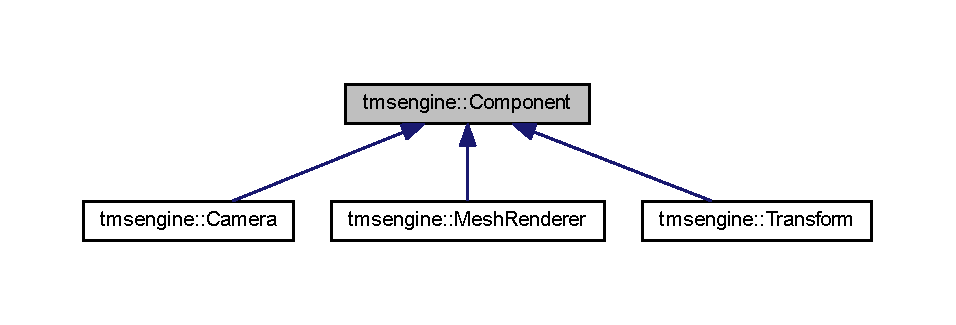
\includegraphics[width=350pt]{classtmsengine_1_1_component__inherit__graph}
\end{center}
\end{figure}
\subsection*{Public Member Functions}
\begin{DoxyCompactItemize}
\item 
virtual \hyperlink{classtmsengine_1_1_component_a764458f5f009e4e01f3c2bdab24b992f}{$\sim$\+Component} ()
\item 
std\+::shared\+\_\+ptr$<$ \hyperlink{classtmsengine_1_1_core}{Core} $>$ \hyperlink{classtmsengine_1_1_component_a80494876282c5e19caeffe6c06c8d4bb}{get\+Core} ()
\item 
std\+::shared\+\_\+ptr$<$ \hyperlink{classtmsengine_1_1_game_object}{Game\+Object} $>$ \hyperlink{classtmsengine_1_1_component_a3df74e0c90f7519e3a9ab541dc77068a}{get\+Game\+Object} ()
\end{DoxyCompactItemize}
\subsection*{Private Member Functions}
\begin{DoxyCompactItemize}
\item 
virtual void \hyperlink{classtmsengine_1_1_component_a71284093fcc0b89f56fe78bd4da1c2e0}{on\+Update} ()
\item 
virtual void \hyperlink{classtmsengine_1_1_component_a73aa3564db299ef43100bd58d7cab65b}{on\+Display} ()
\item 
virtual void \hyperlink{classtmsengine_1_1_component_ae992e9b0c98b569eba13d0274089bc18}{on\+Init} ()
\end{DoxyCompactItemize}
\subsection*{Private Attributes}
\begin{DoxyCompactItemize}
\item 
bool \hyperlink{classtmsengine_1_1_component_a95d8db246b91bef1abcdbb9a38607526}{began}
\item 
std\+::weak\+\_\+ptr$<$ \hyperlink{classtmsengine_1_1_game_object}{Game\+Object} $>$ \hyperlink{classtmsengine_1_1_component_aa7aaf22a0b308873a2ae755d8b653553}{game\+Object}
\end{DoxyCompactItemize}
\subsection*{Friends}
\begin{DoxyCompactItemize}
\item 
class \hyperlink{classtmsengine_1_1_component_a00df87c957d8f7ee0fc51f07a0542f4a}{Game\+Object}
\end{DoxyCompactItemize}


\subsection{Constructor \& Destructor Documentation}
\mbox{\Hypertarget{classtmsengine_1_1_component_a764458f5f009e4e01f3c2bdab24b992f}\label{classtmsengine_1_1_component_a764458f5f009e4e01f3c2bdab24b992f}} 
\index{tmsengine\+::\+Component@{tmsengine\+::\+Component}!````~Component@{$\sim$\+Component}}
\index{````~Component@{$\sim$\+Component}!tmsengine\+::\+Component@{tmsengine\+::\+Component}}
\subsubsection{\texorpdfstring{$\sim$\+Component()}{~Component()}}
{\footnotesize\ttfamily tmsengine\+::\+Component\+::$\sim$\+Component (\begin{DoxyParamCaption}{ }\end{DoxyParamCaption})\hspace{0.3cm}{\ttfamily [virtual]}}



\subsection{Member Function Documentation}
\mbox{\Hypertarget{classtmsengine_1_1_component_a80494876282c5e19caeffe6c06c8d4bb}\label{classtmsengine_1_1_component_a80494876282c5e19caeffe6c06c8d4bb}} 
\index{tmsengine\+::\+Component@{tmsengine\+::\+Component}!get\+Core@{get\+Core}}
\index{get\+Core@{get\+Core}!tmsengine\+::\+Component@{tmsengine\+::\+Component}}
\subsubsection{\texorpdfstring{get\+Core()}{getCore()}}
{\footnotesize\ttfamily std\+::shared\+\_\+ptr$<$ \hyperlink{classtmsengine_1_1_core}{Core} $>$ tmsengine\+::\+Component\+::get\+Core (\begin{DoxyParamCaption}{ }\end{DoxyParamCaption})}

Here is the call graph for this function\+:\nopagebreak
\begin{figure}[H]
\begin{center}
\leavevmode
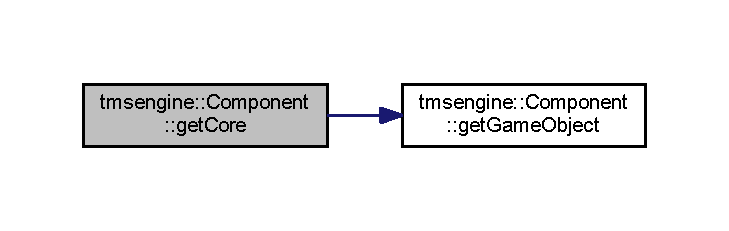
\includegraphics[width=350pt]{classtmsengine_1_1_component_a80494876282c5e19caeffe6c06c8d4bb_cgraph}
\end{center}
\end{figure}
Here is the caller graph for this function\+:\nopagebreak
\begin{figure}[H]
\begin{center}
\leavevmode
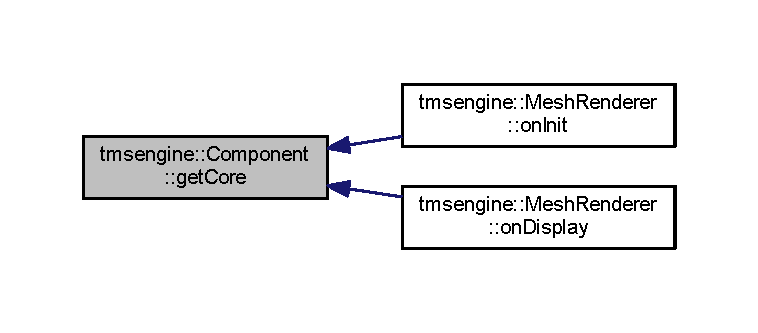
\includegraphics[width=350pt]{classtmsengine_1_1_component_a80494876282c5e19caeffe6c06c8d4bb_icgraph}
\end{center}
\end{figure}
\mbox{\Hypertarget{classtmsengine_1_1_component_a3df74e0c90f7519e3a9ab541dc77068a}\label{classtmsengine_1_1_component_a3df74e0c90f7519e3a9ab541dc77068a}} 
\index{tmsengine\+::\+Component@{tmsengine\+::\+Component}!get\+Game\+Object@{get\+Game\+Object}}
\index{get\+Game\+Object@{get\+Game\+Object}!tmsengine\+::\+Component@{tmsengine\+::\+Component}}
\subsubsection{\texorpdfstring{get\+Game\+Object()}{getGameObject()}}
{\footnotesize\ttfamily std\+::shared\+\_\+ptr$<$ \hyperlink{classtmsengine_1_1_game_object}{Game\+Object} $>$ tmsengine\+::\+Component\+::get\+Game\+Object (\begin{DoxyParamCaption}{ }\end{DoxyParamCaption})}

Here is the caller graph for this function\+:\nopagebreak
\begin{figure}[H]
\begin{center}
\leavevmode
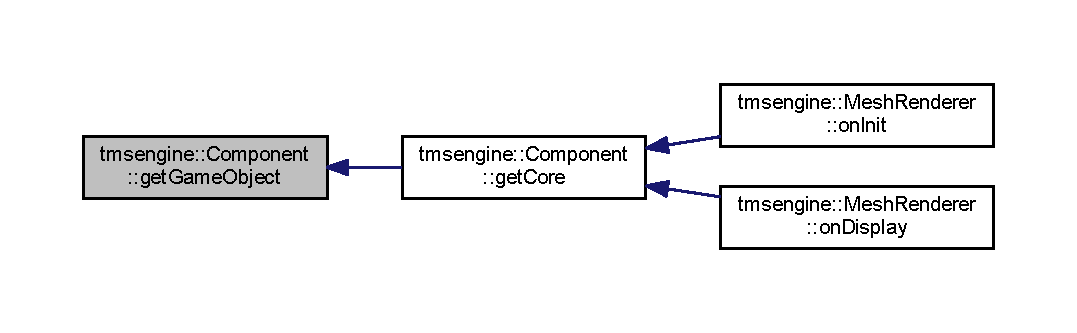
\includegraphics[width=350pt]{classtmsengine_1_1_component_a3df74e0c90f7519e3a9ab541dc77068a_icgraph}
\end{center}
\end{figure}
\mbox{\Hypertarget{classtmsengine_1_1_component_a73aa3564db299ef43100bd58d7cab65b}\label{classtmsengine_1_1_component_a73aa3564db299ef43100bd58d7cab65b}} 
\index{tmsengine\+::\+Component@{tmsengine\+::\+Component}!on\+Display@{on\+Display}}
\index{on\+Display@{on\+Display}!tmsengine\+::\+Component@{tmsengine\+::\+Component}}
\subsubsection{\texorpdfstring{on\+Display()}{onDisplay()}}
{\footnotesize\ttfamily void tmsengine\+::\+Component\+::on\+Display (\begin{DoxyParamCaption}{ }\end{DoxyParamCaption})\hspace{0.3cm}{\ttfamily [private]}, {\ttfamily [virtual]}}



Reimplemented in \hyperlink{classtmsengine_1_1_mesh_renderer_adf77a2164ad1c92e4a310b99624b9fb5}{tmsengine\+::\+Mesh\+Renderer}.

\mbox{\Hypertarget{classtmsengine_1_1_component_ae992e9b0c98b569eba13d0274089bc18}\label{classtmsengine_1_1_component_ae992e9b0c98b569eba13d0274089bc18}} 
\index{tmsengine\+::\+Component@{tmsengine\+::\+Component}!on\+Init@{on\+Init}}
\index{on\+Init@{on\+Init}!tmsengine\+::\+Component@{tmsengine\+::\+Component}}
\subsubsection{\texorpdfstring{on\+Init()}{onInit()}}
{\footnotesize\ttfamily void tmsengine\+::\+Component\+::on\+Init (\begin{DoxyParamCaption}{ }\end{DoxyParamCaption})\hspace{0.3cm}{\ttfamily [private]}, {\ttfamily [virtual]}}



Reimplemented in \hyperlink{classtmsengine_1_1_mesh_renderer_a63ea3f394ba6678a6044068dd4253c97}{tmsengine\+::\+Mesh\+Renderer}, \hyperlink{classtmsengine_1_1_camera_a344a385fcb4cdf0d4d8c78fb5f2cba16}{tmsengine\+::\+Camera}, and \hyperlink{classtmsengine_1_1_transform_a761046214917103b7286e36cde981c00}{tmsengine\+::\+Transform}.

\mbox{\Hypertarget{classtmsengine_1_1_component_a71284093fcc0b89f56fe78bd4da1c2e0}\label{classtmsengine_1_1_component_a71284093fcc0b89f56fe78bd4da1c2e0}} 
\index{tmsengine\+::\+Component@{tmsengine\+::\+Component}!on\+Update@{on\+Update}}
\index{on\+Update@{on\+Update}!tmsengine\+::\+Component@{tmsengine\+::\+Component}}
\subsubsection{\texorpdfstring{on\+Update()}{onUpdate()}}
{\footnotesize\ttfamily void tmsengine\+::\+Component\+::on\+Update (\begin{DoxyParamCaption}{ }\end{DoxyParamCaption})\hspace{0.3cm}{\ttfamily [private]}, {\ttfamily [virtual]}}



\subsection{Friends And Related Function Documentation}
\mbox{\Hypertarget{classtmsengine_1_1_component_a00df87c957d8f7ee0fc51f07a0542f4a}\label{classtmsengine_1_1_component_a00df87c957d8f7ee0fc51f07a0542f4a}} 
\index{tmsengine\+::\+Component@{tmsengine\+::\+Component}!Game\+Object@{Game\+Object}}
\index{Game\+Object@{Game\+Object}!tmsengine\+::\+Component@{tmsengine\+::\+Component}}
\subsubsection{\texorpdfstring{Game\+Object}{GameObject}}
{\footnotesize\ttfamily friend class \hyperlink{classtmsengine_1_1_game_object}{Game\+Object}\hspace{0.3cm}{\ttfamily [friend]}}



\subsection{Member Data Documentation}
\mbox{\Hypertarget{classtmsengine_1_1_component_a95d8db246b91bef1abcdbb9a38607526}\label{classtmsengine_1_1_component_a95d8db246b91bef1abcdbb9a38607526}} 
\index{tmsengine\+::\+Component@{tmsengine\+::\+Component}!began@{began}}
\index{began@{began}!tmsengine\+::\+Component@{tmsengine\+::\+Component}}
\subsubsection{\texorpdfstring{began}{began}}
{\footnotesize\ttfamily bool tmsengine\+::\+Component\+::began\hspace{0.3cm}{\ttfamily [private]}}

\mbox{\Hypertarget{classtmsengine_1_1_component_aa7aaf22a0b308873a2ae755d8b653553}\label{classtmsengine_1_1_component_aa7aaf22a0b308873a2ae755d8b653553}} 
\index{tmsengine\+::\+Component@{tmsengine\+::\+Component}!game\+Object@{game\+Object}}
\index{game\+Object@{game\+Object}!tmsengine\+::\+Component@{tmsengine\+::\+Component}}
\subsubsection{\texorpdfstring{game\+Object}{gameObject}}
{\footnotesize\ttfamily std\+::weak\+\_\+ptr$<$\hyperlink{classtmsengine_1_1_game_object}{Game\+Object}$>$ tmsengine\+::\+Component\+::game\+Object\hspace{0.3cm}{\ttfamily [private]}}



The documentation for this class was generated from the following files\+:\begin{DoxyCompactItemize}
\item 
T\+M\+S\+Engine/\hyperlink{_component_8h}{Component.\+h}\item 
T\+M\+S\+Engine/\hyperlink{_component_8cpp}{Component.\+cpp}\end{DoxyCompactItemize}

\hypertarget{classtmsengine_1_1_core}{}\section{tmsengine\+:\+:Core Class Reference}
\label{classtmsengine_1_1_core}\index{tmsengine\+::\+Core@{tmsengine\+::\+Core}}


{\ttfamily \#include $<$Core.\+h$>$}



Collaboration diagram for tmsengine\+:\+:Core\+:\nopagebreak
\begin{figure}[H]
\begin{center}
\leavevmode
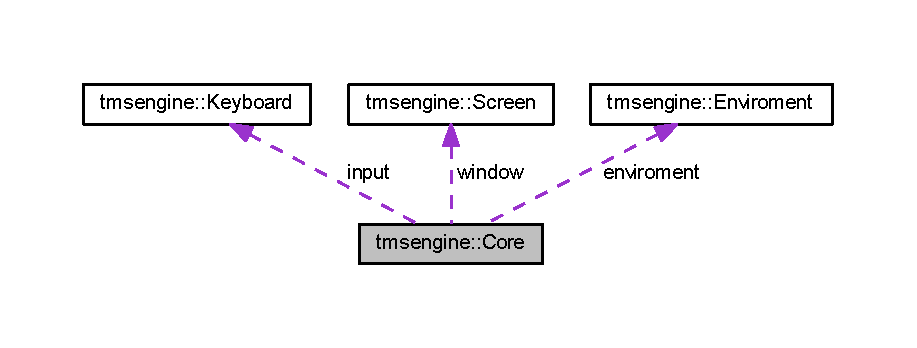
\includegraphics[width=350pt]{classtmsengine_1_1_core__coll__graph}
\end{center}
\end{figure}
\subsection*{Public Member Functions}
\begin{DoxyCompactItemize}
\item 
std\+::shared\+\_\+ptr$<$ \hyperlink{classtmsengine_1_1_game_object}{Game\+Object} $>$ \hyperlink{classtmsengine_1_1_core_a6e341b3f9754d7b9ba9ad49bdf701eb6}{add\+Game\+Object} ()
\item 
void \hyperlink{classtmsengine_1_1_core_af5819357f7cfe0674d4410a606dda3ac}{Start} ()
\item 
{\footnotesize template$<$typename T $>$ }\\std\+::shared\+\_\+ptr$<$ T $>$ \hyperlink{classtmsengine_1_1_core_a45b0f8b3b3edfc6db29707d5b7cce859}{get\+Comp} ()
\end{DoxyCompactItemize}
\subsection*{Static Public Member Functions}
\begin{DoxyCompactItemize}
\item 
static std\+::shared\+\_\+ptr$<$ \hyperlink{classtmsengine_1_1_core}{Core} $>$ \hyperlink{classtmsengine_1_1_core_a6a1dbfaeefd113b669d9a72f828faab7}{initialise} ()
\end{DoxyCompactItemize}
\subsection*{Private Attributes}
\begin{DoxyCompactItemize}
\item 
bool \hyperlink{classtmsengine_1_1_core_a46a10c02877fce53aee7e4939f807ad8}{running}
\item 
std\+::vector$<$ std\+::shared\+\_\+ptr$<$ \hyperlink{classtmsengine_1_1_game_object}{Game\+Object} $>$ $>$ \hyperlink{classtmsengine_1_1_core_afcee2f870370b68981a6ccab00fd2408}{game\+Objects}
\item 
std\+::weak\+\_\+ptr$<$ \hyperlink{classtmsengine_1_1_core}{Core} $>$ \hyperlink{classtmsengine_1_1_core_a8a48e579f54f5ec8c9e795c544c72ecc}{self}
\item 
A\+L\+Cdevice $\ast$ \hyperlink{classtmsengine_1_1_core_a91929ead4dc4bbf21e54e06f1d80408b}{device}
\item 
A\+L\+Ccontext $\ast$ \hyperlink{classtmsengine_1_1_core_a7fc87c5ea5b9b682b8dddef5360e109f}{context}
\item 
\hyperlink{classtmsengine_1_1_keyboard}{Keyboard} \hyperlink{classtmsengine_1_1_core_a58114b7b85229158404c9d087e94e02a}{input}
\item 
\hyperlink{classtmsengine_1_1_enviroment}{Enviroment} \hyperlink{classtmsengine_1_1_core_a5d0429ccd5f0d3bbd18b997e52c0111d}{enviroment}
\item 
\hyperlink{classtmsengine_1_1_screen}{Screen} \hyperlink{classtmsengine_1_1_core_ac0aa6ed388a9fb1fda4c190fc0bb762b}{window}
\end{DoxyCompactItemize}


\subsection{Member Function Documentation}
\mbox{\Hypertarget{classtmsengine_1_1_core_a6e341b3f9754d7b9ba9ad49bdf701eb6}\label{classtmsengine_1_1_core_a6e341b3f9754d7b9ba9ad49bdf701eb6}} 
\index{tmsengine\+::\+Core@{tmsengine\+::\+Core}!add\+Game\+Object@{add\+Game\+Object}}
\index{add\+Game\+Object@{add\+Game\+Object}!tmsengine\+::\+Core@{tmsengine\+::\+Core}}
\subsubsection{\texorpdfstring{add\+Game\+Object()}{addGameObject()}}
{\footnotesize\ttfamily std\+::shared\+\_\+ptr$<$ \hyperlink{classtmsengine_1_1_game_object}{Game\+Object} $>$ tmsengine\+::\+Core\+::add\+Game\+Object (\begin{DoxyParamCaption}{ }\end{DoxyParamCaption})}

\mbox{\Hypertarget{classtmsengine_1_1_core_a45b0f8b3b3edfc6db29707d5b7cce859}\label{classtmsengine_1_1_core_a45b0f8b3b3edfc6db29707d5b7cce859}} 
\index{tmsengine\+::\+Core@{tmsengine\+::\+Core}!get\+Comp@{get\+Comp}}
\index{get\+Comp@{get\+Comp}!tmsengine\+::\+Core@{tmsengine\+::\+Core}}
\subsubsection{\texorpdfstring{get\+Comp()}{getComp()}}
{\footnotesize\ttfamily template$<$typename T $>$ \\
std\+::shared\+\_\+ptr$<$ T $>$ tmsengine\+::\+Core\+::get\+Comp (\begin{DoxyParamCaption}{ }\end{DoxyParamCaption})\hspace{0.3cm}{\ttfamily [inline]}}

\mbox{\Hypertarget{classtmsengine_1_1_core_a6a1dbfaeefd113b669d9a72f828faab7}\label{classtmsengine_1_1_core_a6a1dbfaeefd113b669d9a72f828faab7}} 
\index{tmsengine\+::\+Core@{tmsengine\+::\+Core}!initialise@{initialise}}
\index{initialise@{initialise}!tmsengine\+::\+Core@{tmsengine\+::\+Core}}
\subsubsection{\texorpdfstring{initialise()}{initialise()}}
{\footnotesize\ttfamily std\+::shared\+\_\+ptr$<$ \hyperlink{classtmsengine_1_1_core}{Core} $>$ tmsengine\+::\+Core\+::initialise (\begin{DoxyParamCaption}{ }\end{DoxyParamCaption})\hspace{0.3cm}{\ttfamily [static]}}

\mbox{\Hypertarget{classtmsengine_1_1_core_af5819357f7cfe0674d4410a606dda3ac}\label{classtmsengine_1_1_core_af5819357f7cfe0674d4410a606dda3ac}} 
\index{tmsengine\+::\+Core@{tmsengine\+::\+Core}!Start@{Start}}
\index{Start@{Start}!tmsengine\+::\+Core@{tmsengine\+::\+Core}}
\subsubsection{\texorpdfstring{Start()}{Start()}}
{\footnotesize\ttfamily void tmsengine\+::\+Core\+::\+Start (\begin{DoxyParamCaption}{ }\end{DoxyParamCaption})}

Here is the call graph for this function\+:\nopagebreak
\begin{figure}[H]
\begin{center}
\leavevmode
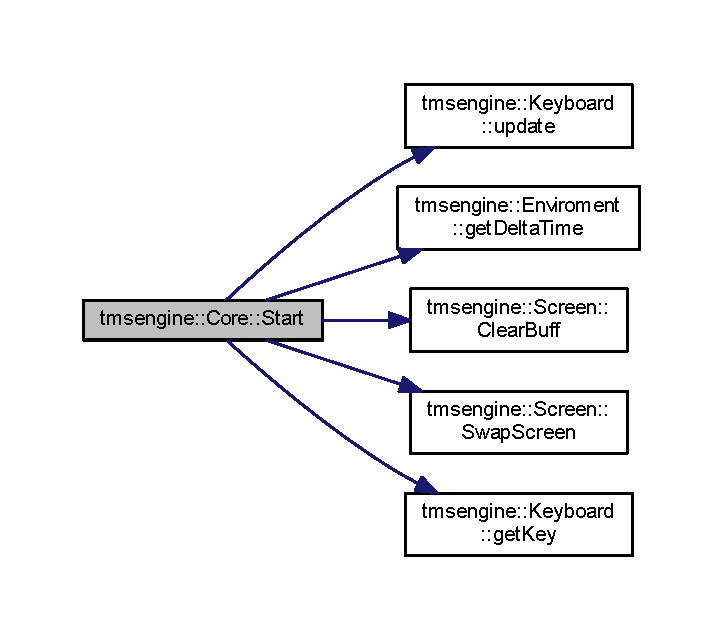
\includegraphics[width=347pt]{classtmsengine_1_1_core_af5819357f7cfe0674d4410a606dda3ac_cgraph}
\end{center}
\end{figure}


\subsection{Member Data Documentation}
\mbox{\Hypertarget{classtmsengine_1_1_core_a7fc87c5ea5b9b682b8dddef5360e109f}\label{classtmsengine_1_1_core_a7fc87c5ea5b9b682b8dddef5360e109f}} 
\index{tmsengine\+::\+Core@{tmsengine\+::\+Core}!context@{context}}
\index{context@{context}!tmsengine\+::\+Core@{tmsengine\+::\+Core}}
\subsubsection{\texorpdfstring{context}{context}}
{\footnotesize\ttfamily A\+L\+Ccontext$\ast$ tmsengine\+::\+Core\+::context\hspace{0.3cm}{\ttfamily [private]}}

\mbox{\Hypertarget{classtmsengine_1_1_core_a91929ead4dc4bbf21e54e06f1d80408b}\label{classtmsengine_1_1_core_a91929ead4dc4bbf21e54e06f1d80408b}} 
\index{tmsengine\+::\+Core@{tmsengine\+::\+Core}!device@{device}}
\index{device@{device}!tmsengine\+::\+Core@{tmsengine\+::\+Core}}
\subsubsection{\texorpdfstring{device}{device}}
{\footnotesize\ttfamily A\+L\+Cdevice$\ast$ tmsengine\+::\+Core\+::device\hspace{0.3cm}{\ttfamily [private]}}

\mbox{\Hypertarget{classtmsengine_1_1_core_a5d0429ccd5f0d3bbd18b997e52c0111d}\label{classtmsengine_1_1_core_a5d0429ccd5f0d3bbd18b997e52c0111d}} 
\index{tmsengine\+::\+Core@{tmsengine\+::\+Core}!enviroment@{enviroment}}
\index{enviroment@{enviroment}!tmsengine\+::\+Core@{tmsengine\+::\+Core}}
\subsubsection{\texorpdfstring{enviroment}{enviroment}}
{\footnotesize\ttfamily \hyperlink{classtmsengine_1_1_enviroment}{Enviroment} tmsengine\+::\+Core\+::enviroment\hspace{0.3cm}{\ttfamily [private]}}

\mbox{\Hypertarget{classtmsengine_1_1_core_afcee2f870370b68981a6ccab00fd2408}\label{classtmsengine_1_1_core_afcee2f870370b68981a6ccab00fd2408}} 
\index{tmsengine\+::\+Core@{tmsengine\+::\+Core}!game\+Objects@{game\+Objects}}
\index{game\+Objects@{game\+Objects}!tmsengine\+::\+Core@{tmsengine\+::\+Core}}
\subsubsection{\texorpdfstring{game\+Objects}{gameObjects}}
{\footnotesize\ttfamily std\+::vector$<$std\+::shared\+\_\+ptr$<$\hyperlink{classtmsengine_1_1_game_object}{Game\+Object}$>$ $>$ tmsengine\+::\+Core\+::game\+Objects\hspace{0.3cm}{\ttfamily [private]}}

\mbox{\Hypertarget{classtmsengine_1_1_core_a58114b7b85229158404c9d087e94e02a}\label{classtmsengine_1_1_core_a58114b7b85229158404c9d087e94e02a}} 
\index{tmsengine\+::\+Core@{tmsengine\+::\+Core}!input@{input}}
\index{input@{input}!tmsengine\+::\+Core@{tmsengine\+::\+Core}}
\subsubsection{\texorpdfstring{input}{input}}
{\footnotesize\ttfamily \hyperlink{classtmsengine_1_1_keyboard}{Keyboard} tmsengine\+::\+Core\+::input\hspace{0.3cm}{\ttfamily [private]}}

\mbox{\Hypertarget{classtmsengine_1_1_core_a46a10c02877fce53aee7e4939f807ad8}\label{classtmsengine_1_1_core_a46a10c02877fce53aee7e4939f807ad8}} 
\index{tmsengine\+::\+Core@{tmsengine\+::\+Core}!running@{running}}
\index{running@{running}!tmsengine\+::\+Core@{tmsengine\+::\+Core}}
\subsubsection{\texorpdfstring{running}{running}}
{\footnotesize\ttfamily bool tmsengine\+::\+Core\+::running\hspace{0.3cm}{\ttfamily [private]}}

\mbox{\Hypertarget{classtmsengine_1_1_core_a8a48e579f54f5ec8c9e795c544c72ecc}\label{classtmsengine_1_1_core_a8a48e579f54f5ec8c9e795c544c72ecc}} 
\index{tmsengine\+::\+Core@{tmsengine\+::\+Core}!self@{self}}
\index{self@{self}!tmsengine\+::\+Core@{tmsengine\+::\+Core}}
\subsubsection{\texorpdfstring{self}{self}}
{\footnotesize\ttfamily std\+::weak\+\_\+ptr$<$\hyperlink{classtmsengine_1_1_core}{Core}$>$ tmsengine\+::\+Core\+::self\hspace{0.3cm}{\ttfamily [private]}}

\mbox{\Hypertarget{classtmsengine_1_1_core_ac0aa6ed388a9fb1fda4c190fc0bb762b}\label{classtmsengine_1_1_core_ac0aa6ed388a9fb1fda4c190fc0bb762b}} 
\index{tmsengine\+::\+Core@{tmsengine\+::\+Core}!window@{window}}
\index{window@{window}!tmsengine\+::\+Core@{tmsengine\+::\+Core}}
\subsubsection{\texorpdfstring{window}{window}}
{\footnotesize\ttfamily \hyperlink{classtmsengine_1_1_screen}{Screen} tmsengine\+::\+Core\+::window\hspace{0.3cm}{\ttfamily [private]}}



The documentation for this class was generated from the following files\+:\begin{DoxyCompactItemize}
\item 
T\+M\+S\+Engine/\hyperlink{_core_8h}{Core.\+h}\item 
T\+M\+S\+Engine/\hyperlink{_core_8cpp}{Core.\+cpp}\end{DoxyCompactItemize}

\hypertarget{classtmsengine_1_1_enviroment}{}\section{tmsengine\+:\+:Enviroment Class Reference}
\label{classtmsengine_1_1_enviroment}\index{tmsengine\+::\+Enviroment@{tmsengine\+::\+Enviroment}}


{\ttfamily \#include $<$Enviroment.\+h$>$}

\subsection*{Public Member Functions}
\begin{DoxyCompactItemize}
\item 
void \hyperlink{classtmsengine_1_1_enviroment_ae82cd04e139ac869bdb6a1b41a28c830}{init} ()
\item 
float \hyperlink{classtmsengine_1_1_enviroment_aaa6d260aca99eb32d5ee96771fe34a01}{get\+Delta\+Time} ()
\end{DoxyCompactItemize}
\subsection*{Private Attributes}
\begin{DoxyCompactItemize}
\item 
float \hyperlink{classtmsengine_1_1_enviroment_a6481f99308483a38e2a130f775767dd3}{delta\+Time} = 0
\item 
float \hyperlink{classtmsengine_1_1_enviroment_a54af05c4adbbd3fe48826def702930c6}{last\+Time}
\item 
float \hyperlink{classtmsengine_1_1_enviroment_ae84ce684b9aa9f35f2bfc75bf22ab924}{time}
\item 
float \hyperlink{classtmsengine_1_1_enviroment_a8beebe427c5a407990fbd3045b16a2c6}{difference}
\item 
float \hyperlink{classtmsengine_1_1_enviroment_a69006efe0a003b6190a4117585c90f99}{ideal\+Time}
\end{DoxyCompactItemize}


\subsection{Member Function Documentation}
\mbox{\Hypertarget{classtmsengine_1_1_enviroment_aaa6d260aca99eb32d5ee96771fe34a01}\label{classtmsengine_1_1_enviroment_aaa6d260aca99eb32d5ee96771fe34a01}} 
\index{tmsengine\+::\+Enviroment@{tmsengine\+::\+Enviroment}!get\+Delta\+Time@{get\+Delta\+Time}}
\index{get\+Delta\+Time@{get\+Delta\+Time}!tmsengine\+::\+Enviroment@{tmsengine\+::\+Enviroment}}
\subsubsection{\texorpdfstring{get\+Delta\+Time()}{getDeltaTime()}}
{\footnotesize\ttfamily float tmsengine\+::\+Enviroment\+::get\+Delta\+Time (\begin{DoxyParamCaption}{ }\end{DoxyParamCaption})}

Here is the caller graph for this function\+:\nopagebreak
\begin{figure}[H]
\begin{center}
\leavevmode
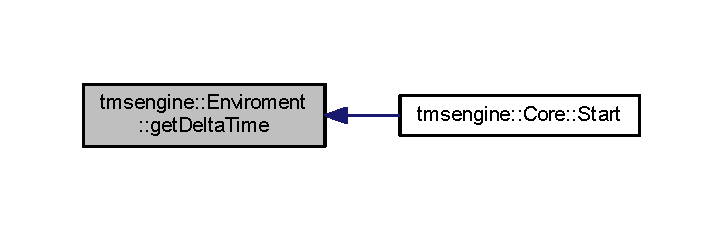
\includegraphics[width=347pt]{classtmsengine_1_1_enviroment_aaa6d260aca99eb32d5ee96771fe34a01_icgraph}
\end{center}
\end{figure}
\mbox{\Hypertarget{classtmsengine_1_1_enviroment_ae82cd04e139ac869bdb6a1b41a28c830}\label{classtmsengine_1_1_enviroment_ae82cd04e139ac869bdb6a1b41a28c830}} 
\index{tmsengine\+::\+Enviroment@{tmsengine\+::\+Enviroment}!init@{init}}
\index{init@{init}!tmsengine\+::\+Enviroment@{tmsengine\+::\+Enviroment}}
\subsubsection{\texorpdfstring{init()}{init()}}
{\footnotesize\ttfamily void tmsengine\+::\+Enviroment\+::init (\begin{DoxyParamCaption}{ }\end{DoxyParamCaption})}



\subsection{Member Data Documentation}
\mbox{\Hypertarget{classtmsengine_1_1_enviroment_a6481f99308483a38e2a130f775767dd3}\label{classtmsengine_1_1_enviroment_a6481f99308483a38e2a130f775767dd3}} 
\index{tmsengine\+::\+Enviroment@{tmsengine\+::\+Enviroment}!delta\+Time@{delta\+Time}}
\index{delta\+Time@{delta\+Time}!tmsengine\+::\+Enviroment@{tmsengine\+::\+Enviroment}}
\subsubsection{\texorpdfstring{delta\+Time}{deltaTime}}
{\footnotesize\ttfamily float tmsengine\+::\+Enviroment\+::delta\+Time = 0\hspace{0.3cm}{\ttfamily [private]}}

\mbox{\Hypertarget{classtmsengine_1_1_enviroment_a8beebe427c5a407990fbd3045b16a2c6}\label{classtmsengine_1_1_enviroment_a8beebe427c5a407990fbd3045b16a2c6}} 
\index{tmsengine\+::\+Enviroment@{tmsengine\+::\+Enviroment}!difference@{difference}}
\index{difference@{difference}!tmsengine\+::\+Enviroment@{tmsengine\+::\+Enviroment}}
\subsubsection{\texorpdfstring{difference}{difference}}
{\footnotesize\ttfamily float tmsengine\+::\+Enviroment\+::difference\hspace{0.3cm}{\ttfamily [private]}}

\mbox{\Hypertarget{classtmsengine_1_1_enviroment_a69006efe0a003b6190a4117585c90f99}\label{classtmsengine_1_1_enviroment_a69006efe0a003b6190a4117585c90f99}} 
\index{tmsengine\+::\+Enviroment@{tmsengine\+::\+Enviroment}!ideal\+Time@{ideal\+Time}}
\index{ideal\+Time@{ideal\+Time}!tmsengine\+::\+Enviroment@{tmsengine\+::\+Enviroment}}
\subsubsection{\texorpdfstring{ideal\+Time}{idealTime}}
{\footnotesize\ttfamily float tmsengine\+::\+Enviroment\+::ideal\+Time\hspace{0.3cm}{\ttfamily [private]}}

\mbox{\Hypertarget{classtmsengine_1_1_enviroment_a54af05c4adbbd3fe48826def702930c6}\label{classtmsengine_1_1_enviroment_a54af05c4adbbd3fe48826def702930c6}} 
\index{tmsengine\+::\+Enviroment@{tmsengine\+::\+Enviroment}!last\+Time@{last\+Time}}
\index{last\+Time@{last\+Time}!tmsengine\+::\+Enviroment@{tmsengine\+::\+Enviroment}}
\subsubsection{\texorpdfstring{last\+Time}{lastTime}}
{\footnotesize\ttfamily float tmsengine\+::\+Enviroment\+::last\+Time\hspace{0.3cm}{\ttfamily [private]}}

\mbox{\Hypertarget{classtmsengine_1_1_enviroment_ae84ce684b9aa9f35f2bfc75bf22ab924}\label{classtmsengine_1_1_enviroment_ae84ce684b9aa9f35f2bfc75bf22ab924}} 
\index{tmsengine\+::\+Enviroment@{tmsengine\+::\+Enviroment}!time@{time}}
\index{time@{time}!tmsengine\+::\+Enviroment@{tmsengine\+::\+Enviroment}}
\subsubsection{\texorpdfstring{time}{time}}
{\footnotesize\ttfamily float tmsengine\+::\+Enviroment\+::time\hspace{0.3cm}{\ttfamily [private]}}



The documentation for this class was generated from the following files\+:\begin{DoxyCompactItemize}
\item 
T\+M\+S\+Engine/\hyperlink{_enviroment_8h}{Enviroment.\+h}\item 
T\+M\+S\+Engine/\hyperlink{_enviroment_8cpp}{Enviroment.\+cpp}\end{DoxyCompactItemize}

\hypertarget{classtmsengine_1_1_game_object}{}\section{tmsengine\+:\+:Game\+Object Class Reference}
\label{classtmsengine_1_1_game_object}\index{tmsengine\+::\+Game\+Object@{tmsengine\+::\+Game\+Object}}


{\ttfamily \#include $<$Game\+Object.\+h$>$}

\subsection*{Public Member Functions}
\begin{DoxyCompactItemize}
\item 
void \hyperlink{classtmsengine_1_1_game_object_adde904518de57fa132493e07b7b0cda7}{update} ()
\item 
void \hyperlink{classtmsengine_1_1_game_object_af94d4e76cf2aa823071178132ecf1060}{display} ()
\item 
{\footnotesize template$<$typename T $>$ }\\std\+::shared\+\_\+ptr$<$ T $>$ \hyperlink{classtmsengine_1_1_game_object_a55aab957aab04d2fd400a03f4c32dfee}{Add\+Component} ()
\item 
{\footnotesize template$<$typename T $>$ }\\std\+::shared\+\_\+ptr$<$ T $>$ \hyperlink{classtmsengine_1_1_game_object_a6100faa614234f00062074ef31be7bc3}{Get\+Component} ()
\item 
std\+::shared\+\_\+ptr$<$ \hyperlink{classtmsengine_1_1_core}{Core} $>$ \hyperlink{classtmsengine_1_1_game_object_abcaf58a2195a319064266cbac0bf74d6}{get\+Core} ()
\end{DoxyCompactItemize}
\subsection*{Private Attributes}
\begin{DoxyCompactItemize}
\item 
std\+::vector$<$ std\+::shared\+\_\+ptr$<$ \hyperlink{classtmsengine_1_1_component}{Component} $>$ $>$ \hyperlink{classtmsengine_1_1_game_object_a94c0947df66676bfce83cd1d28ef8a32}{components}
\item 
std\+::weak\+\_\+ptr$<$ \hyperlink{classtmsengine_1_1_core}{Core} $>$ \hyperlink{classtmsengine_1_1_game_object_ae7f1027d4e1fdc66ec0a5d383136165b}{core}
\item 
std\+::weak\+\_\+ptr$<$ \hyperlink{classtmsengine_1_1_game_object}{Game\+Object} $>$ \hyperlink{classtmsengine_1_1_game_object_a5b74bdb7c894b24eaf4ef56610b5f2e6}{self}
\end{DoxyCompactItemize}
\subsection*{Friends}
\begin{DoxyCompactItemize}
\item 
class \hyperlink{classtmsengine_1_1_game_object_a4107254ac74f90d4f91e810d755b98c2}{Core}
\end{DoxyCompactItemize}


\subsection{Member Function Documentation}
\mbox{\Hypertarget{classtmsengine_1_1_game_object_a55aab957aab04d2fd400a03f4c32dfee}\label{classtmsengine_1_1_game_object_a55aab957aab04d2fd400a03f4c32dfee}} 
\index{tmsengine\+::\+Game\+Object@{tmsengine\+::\+Game\+Object}!Add\+Component@{Add\+Component}}
\index{Add\+Component@{Add\+Component}!tmsengine\+::\+Game\+Object@{tmsengine\+::\+Game\+Object}}
\subsubsection{\texorpdfstring{Add\+Component()}{AddComponent()}}
{\footnotesize\ttfamily template$<$typename T $>$ \\
std\+::shared\+\_\+ptr$<$T$>$ tmsengine\+::\+Game\+Object\+::\+Add\+Component (\begin{DoxyParamCaption}{ }\end{DoxyParamCaption})\hspace{0.3cm}{\ttfamily [inline]}}

\mbox{\Hypertarget{classtmsengine_1_1_game_object_af94d4e76cf2aa823071178132ecf1060}\label{classtmsengine_1_1_game_object_af94d4e76cf2aa823071178132ecf1060}} 
\index{tmsengine\+::\+Game\+Object@{tmsengine\+::\+Game\+Object}!display@{display}}
\index{display@{display}!tmsengine\+::\+Game\+Object@{tmsengine\+::\+Game\+Object}}
\subsubsection{\texorpdfstring{display()}{display()}}
{\footnotesize\ttfamily void tmsengine\+::\+Game\+Object\+::display (\begin{DoxyParamCaption}{ }\end{DoxyParamCaption})}

\mbox{\Hypertarget{classtmsengine_1_1_game_object_a6100faa614234f00062074ef31be7bc3}\label{classtmsengine_1_1_game_object_a6100faa614234f00062074ef31be7bc3}} 
\index{tmsengine\+::\+Game\+Object@{tmsengine\+::\+Game\+Object}!Get\+Component@{Get\+Component}}
\index{Get\+Component@{Get\+Component}!tmsengine\+::\+Game\+Object@{tmsengine\+::\+Game\+Object}}
\subsubsection{\texorpdfstring{Get\+Component()}{GetComponent()}}
{\footnotesize\ttfamily template$<$typename T $>$ \\
std\+::shared\+\_\+ptr$<$T$>$ tmsengine\+::\+Game\+Object\+::\+Get\+Component (\begin{DoxyParamCaption}{ }\end{DoxyParamCaption})\hspace{0.3cm}{\ttfamily [inline]}}

\mbox{\Hypertarget{classtmsengine_1_1_game_object_abcaf58a2195a319064266cbac0bf74d6}\label{classtmsengine_1_1_game_object_abcaf58a2195a319064266cbac0bf74d6}} 
\index{tmsengine\+::\+Game\+Object@{tmsengine\+::\+Game\+Object}!get\+Core@{get\+Core}}
\index{get\+Core@{get\+Core}!tmsengine\+::\+Game\+Object@{tmsengine\+::\+Game\+Object}}
\subsubsection{\texorpdfstring{get\+Core()}{getCore()}}
{\footnotesize\ttfamily std\+::shared\+\_\+ptr$<$ \hyperlink{classtmsengine_1_1_core}{Core} $>$ tmsengine\+::\+Game\+Object\+::get\+Core (\begin{DoxyParamCaption}{ }\end{DoxyParamCaption})}

\mbox{\Hypertarget{classtmsengine_1_1_game_object_adde904518de57fa132493e07b7b0cda7}\label{classtmsengine_1_1_game_object_adde904518de57fa132493e07b7b0cda7}} 
\index{tmsengine\+::\+Game\+Object@{tmsengine\+::\+Game\+Object}!update@{update}}
\index{update@{update}!tmsengine\+::\+Game\+Object@{tmsengine\+::\+Game\+Object}}
\subsubsection{\texorpdfstring{update()}{update()}}
{\footnotesize\ttfamily void tmsengine\+::\+Game\+Object\+::update (\begin{DoxyParamCaption}{ }\end{DoxyParamCaption})}



\subsection{Friends And Related Function Documentation}
\mbox{\Hypertarget{classtmsengine_1_1_game_object_a4107254ac74f90d4f91e810d755b98c2}\label{classtmsengine_1_1_game_object_a4107254ac74f90d4f91e810d755b98c2}} 
\index{tmsengine\+::\+Game\+Object@{tmsengine\+::\+Game\+Object}!Core@{Core}}
\index{Core@{Core}!tmsengine\+::\+Game\+Object@{tmsengine\+::\+Game\+Object}}
\subsubsection{\texorpdfstring{Core}{Core}}
{\footnotesize\ttfamily friend class \hyperlink{classtmsengine_1_1_core}{Core}\hspace{0.3cm}{\ttfamily [friend]}}



\subsection{Member Data Documentation}
\mbox{\Hypertarget{classtmsengine_1_1_game_object_a94c0947df66676bfce83cd1d28ef8a32}\label{classtmsengine_1_1_game_object_a94c0947df66676bfce83cd1d28ef8a32}} 
\index{tmsengine\+::\+Game\+Object@{tmsengine\+::\+Game\+Object}!components@{components}}
\index{components@{components}!tmsengine\+::\+Game\+Object@{tmsengine\+::\+Game\+Object}}
\subsubsection{\texorpdfstring{components}{components}}
{\footnotesize\ttfamily std\+::vector$<$std\+::shared\+\_\+ptr$<$\hyperlink{classtmsengine_1_1_component}{Component}$>$ $>$ tmsengine\+::\+Game\+Object\+::components\hspace{0.3cm}{\ttfamily [private]}}

\mbox{\Hypertarget{classtmsengine_1_1_game_object_ae7f1027d4e1fdc66ec0a5d383136165b}\label{classtmsengine_1_1_game_object_ae7f1027d4e1fdc66ec0a5d383136165b}} 
\index{tmsengine\+::\+Game\+Object@{tmsengine\+::\+Game\+Object}!core@{core}}
\index{core@{core}!tmsengine\+::\+Game\+Object@{tmsengine\+::\+Game\+Object}}
\subsubsection{\texorpdfstring{core}{core}}
{\footnotesize\ttfamily std\+::weak\+\_\+ptr$<$\hyperlink{classtmsengine_1_1_core}{Core}$>$ tmsengine\+::\+Game\+Object\+::core\hspace{0.3cm}{\ttfamily [private]}}

\mbox{\Hypertarget{classtmsengine_1_1_game_object_a5b74bdb7c894b24eaf4ef56610b5f2e6}\label{classtmsengine_1_1_game_object_a5b74bdb7c894b24eaf4ef56610b5f2e6}} 
\index{tmsengine\+::\+Game\+Object@{tmsengine\+::\+Game\+Object}!self@{self}}
\index{self@{self}!tmsengine\+::\+Game\+Object@{tmsengine\+::\+Game\+Object}}
\subsubsection{\texorpdfstring{self}{self}}
{\footnotesize\ttfamily std\+::weak\+\_\+ptr$<$\hyperlink{classtmsengine_1_1_game_object}{Game\+Object}$>$ tmsengine\+::\+Game\+Object\+::self\hspace{0.3cm}{\ttfamily [private]}}



The documentation for this class was generated from the following files\+:\begin{DoxyCompactItemize}
\item 
T\+M\+S\+Engine/\hyperlink{_game_object_8h}{Game\+Object.\+h}\item 
T\+M\+S\+Engine/\hyperlink{_game_object_8cpp}{Game\+Object.\+cpp}\end{DoxyCompactItemize}

\hypertarget{classtmsengine_1_1_keyboard}{}\section{tmsengine\+:\+:Keyboard Class Reference}
\label{classtmsengine_1_1_keyboard}\index{tmsengine\+::\+Keyboard@{tmsengine\+::\+Keyboard}}


{\ttfamily \#include $<$Keyboard.\+h$>$}

\subsection*{Public Member Functions}
\begin{DoxyCompactItemize}
\item 
void \hyperlink{classtmsengine_1_1_keyboard_a4f06c5af1c66b1068eb588fffa90aea2}{init} ()
\item 
void \hyperlink{classtmsengine_1_1_keyboard_a61b823821007a6583b277cf0622b201f}{update} ()
\item 
bool \hyperlink{classtmsengine_1_1_keyboard_ab7baeae12cffe8f588fdf5a1227f09ba}{get\+Key} (S\+D\+L\+\_\+\+Scancode key\+Code)
\item 
bool \hyperlink{classtmsengine_1_1_keyboard_a41ea249e18f2422a1de274dd51df0e8c}{get\+Key\+Down} (S\+D\+L\+\_\+\+Scancode key\+Code)
\item 
bool \hyperlink{classtmsengine_1_1_keyboard_a9de47cf02ce1c2c7c1652ac94ea19f5b}{get\+Key\+Up} (S\+D\+L\+\_\+\+Scancode key\+Code)
\end{DoxyCompactItemize}
\subsection*{Private Attributes}
\begin{DoxyCompactItemize}
\item 
int \hyperlink{classtmsengine_1_1_keyboard_ab5325c0c186bdb26b7768e394b0c155a}{key\+Codes}
\item 
Uint8 $\ast$ \hyperlink{classtmsengine_1_1_keyboard_ab35375d64c025c56b604e923e0287ea9}{curr\+Key}
\item 
Uint8 $\ast$ \hyperlink{classtmsengine_1_1_keyboard_a18f801428d84502e6df1b669c0ca5cb4}{prev\+Key}
\end{DoxyCompactItemize}


\subsection{Member Function Documentation}
\mbox{\Hypertarget{classtmsengine_1_1_keyboard_ab7baeae12cffe8f588fdf5a1227f09ba}\label{classtmsengine_1_1_keyboard_ab7baeae12cffe8f588fdf5a1227f09ba}} 
\index{tmsengine\+::\+Keyboard@{tmsengine\+::\+Keyboard}!get\+Key@{get\+Key}}
\index{get\+Key@{get\+Key}!tmsengine\+::\+Keyboard@{tmsengine\+::\+Keyboard}}
\subsubsection{\texorpdfstring{get\+Key()}{getKey()}}
{\footnotesize\ttfamily bool tmsengine\+::\+Keyboard\+::get\+Key (\begin{DoxyParamCaption}\item[{S\+D\+L\+\_\+\+Scancode}]{key\+Code }\end{DoxyParamCaption})}

Here is the caller graph for this function\+:\nopagebreak
\begin{figure}[H]
\begin{center}
\leavevmode
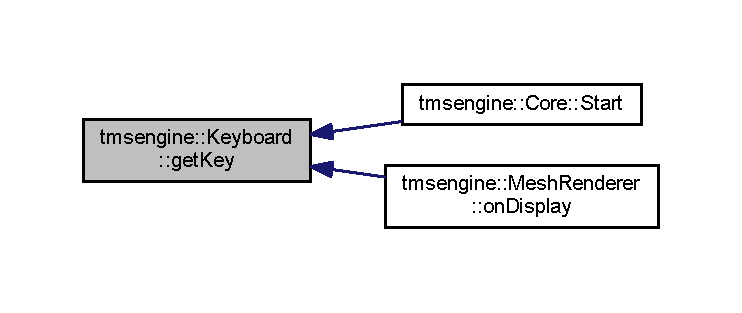
\includegraphics[width=350pt]{classtmsengine_1_1_keyboard_ab7baeae12cffe8f588fdf5a1227f09ba_icgraph}
\end{center}
\end{figure}
\mbox{\Hypertarget{classtmsengine_1_1_keyboard_a41ea249e18f2422a1de274dd51df0e8c}\label{classtmsengine_1_1_keyboard_a41ea249e18f2422a1de274dd51df0e8c}} 
\index{tmsengine\+::\+Keyboard@{tmsengine\+::\+Keyboard}!get\+Key\+Down@{get\+Key\+Down}}
\index{get\+Key\+Down@{get\+Key\+Down}!tmsengine\+::\+Keyboard@{tmsengine\+::\+Keyboard}}
\subsubsection{\texorpdfstring{get\+Key\+Down()}{getKeyDown()}}
{\footnotesize\ttfamily bool tmsengine\+::\+Keyboard\+::get\+Key\+Down (\begin{DoxyParamCaption}\item[{S\+D\+L\+\_\+\+Scancode}]{key\+Code }\end{DoxyParamCaption})}

\mbox{\Hypertarget{classtmsengine_1_1_keyboard_a9de47cf02ce1c2c7c1652ac94ea19f5b}\label{classtmsengine_1_1_keyboard_a9de47cf02ce1c2c7c1652ac94ea19f5b}} 
\index{tmsengine\+::\+Keyboard@{tmsengine\+::\+Keyboard}!get\+Key\+Up@{get\+Key\+Up}}
\index{get\+Key\+Up@{get\+Key\+Up}!tmsengine\+::\+Keyboard@{tmsengine\+::\+Keyboard}}
\subsubsection{\texorpdfstring{get\+Key\+Up()}{getKeyUp()}}
{\footnotesize\ttfamily bool tmsengine\+::\+Keyboard\+::get\+Key\+Up (\begin{DoxyParamCaption}\item[{S\+D\+L\+\_\+\+Scancode}]{key\+Code }\end{DoxyParamCaption})}

\mbox{\Hypertarget{classtmsengine_1_1_keyboard_a4f06c5af1c66b1068eb588fffa90aea2}\label{classtmsengine_1_1_keyboard_a4f06c5af1c66b1068eb588fffa90aea2}} 
\index{tmsengine\+::\+Keyboard@{tmsengine\+::\+Keyboard}!init@{init}}
\index{init@{init}!tmsengine\+::\+Keyboard@{tmsengine\+::\+Keyboard}}
\subsubsection{\texorpdfstring{init()}{init()}}
{\footnotesize\ttfamily void tmsengine\+::\+Keyboard\+::init (\begin{DoxyParamCaption}{ }\end{DoxyParamCaption})}

Here is the caller graph for this function\+:\nopagebreak
\begin{figure}[H]
\begin{center}
\leavevmode
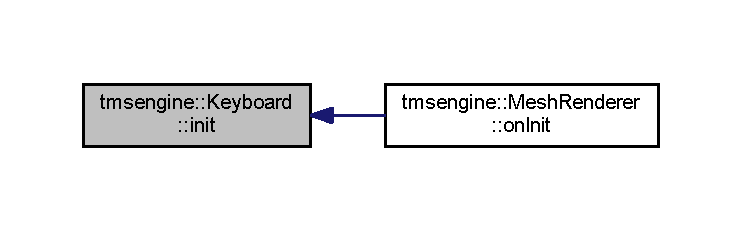
\includegraphics[width=350pt]{classtmsengine_1_1_keyboard_a4f06c5af1c66b1068eb588fffa90aea2_icgraph}
\end{center}
\end{figure}
\mbox{\Hypertarget{classtmsengine_1_1_keyboard_a61b823821007a6583b277cf0622b201f}\label{classtmsengine_1_1_keyboard_a61b823821007a6583b277cf0622b201f}} 
\index{tmsengine\+::\+Keyboard@{tmsengine\+::\+Keyboard}!update@{update}}
\index{update@{update}!tmsengine\+::\+Keyboard@{tmsengine\+::\+Keyboard}}
\subsubsection{\texorpdfstring{update()}{update()}}
{\footnotesize\ttfamily void tmsengine\+::\+Keyboard\+::update (\begin{DoxyParamCaption}{ }\end{DoxyParamCaption})}

Here is the caller graph for this function\+:\nopagebreak
\begin{figure}[H]
\begin{center}
\leavevmode
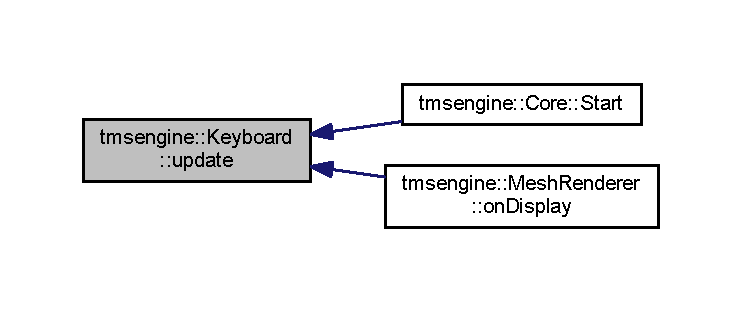
\includegraphics[width=350pt]{classtmsengine_1_1_keyboard_a61b823821007a6583b277cf0622b201f_icgraph}
\end{center}
\end{figure}


\subsection{Member Data Documentation}
\mbox{\Hypertarget{classtmsengine_1_1_keyboard_ab35375d64c025c56b604e923e0287ea9}\label{classtmsengine_1_1_keyboard_ab35375d64c025c56b604e923e0287ea9}} 
\index{tmsengine\+::\+Keyboard@{tmsengine\+::\+Keyboard}!curr\+Key@{curr\+Key}}
\index{curr\+Key@{curr\+Key}!tmsengine\+::\+Keyboard@{tmsengine\+::\+Keyboard}}
\subsubsection{\texorpdfstring{curr\+Key}{currKey}}
{\footnotesize\ttfamily Uint8$\ast$ tmsengine\+::\+Keyboard\+::curr\+Key\hspace{0.3cm}{\ttfamily [private]}}

\mbox{\Hypertarget{classtmsengine_1_1_keyboard_ab5325c0c186bdb26b7768e394b0c155a}\label{classtmsengine_1_1_keyboard_ab5325c0c186bdb26b7768e394b0c155a}} 
\index{tmsengine\+::\+Keyboard@{tmsengine\+::\+Keyboard}!key\+Codes@{key\+Codes}}
\index{key\+Codes@{key\+Codes}!tmsengine\+::\+Keyboard@{tmsengine\+::\+Keyboard}}
\subsubsection{\texorpdfstring{key\+Codes}{keyCodes}}
{\footnotesize\ttfamily int tmsengine\+::\+Keyboard\+::key\+Codes\hspace{0.3cm}{\ttfamily [private]}}

\mbox{\Hypertarget{classtmsengine_1_1_keyboard_a18f801428d84502e6df1b669c0ca5cb4}\label{classtmsengine_1_1_keyboard_a18f801428d84502e6df1b669c0ca5cb4}} 
\index{tmsengine\+::\+Keyboard@{tmsengine\+::\+Keyboard}!prev\+Key@{prev\+Key}}
\index{prev\+Key@{prev\+Key}!tmsengine\+::\+Keyboard@{tmsengine\+::\+Keyboard}}
\subsubsection{\texorpdfstring{prev\+Key}{prevKey}}
{\footnotesize\ttfamily Uint8$\ast$ tmsengine\+::\+Keyboard\+::prev\+Key\hspace{0.3cm}{\ttfamily [private]}}



The documentation for this class was generated from the following files\+:\begin{DoxyCompactItemize}
\item 
T\+M\+S\+Engine/\hyperlink{_keyboard_8h}{Keyboard.\+h}\item 
T\+M\+S\+Engine/\hyperlink{_keyboard_8cpp}{Keyboard.\+cpp}\end{DoxyCompactItemize}

\hypertarget{class_material}{}\section{Material Class Reference}
\label{class_material}\index{Material@{Material}}


{\ttfamily \#include $<$Material.\+h$>$}

\subsection*{Public Member Functions}
\begin{DoxyCompactItemize}
\item 
void \hyperlink{class_material_af22f2c958c2bc0f1e34f0b965df7bc6f}{set\+Shader} (std\+::weak\+\_\+ptr$<$ \hyperlink{class_shader}{Shader} $>$\hyperlink{class_material_a0acf8a8f7e55ddddcef3391e68ea74c5}{shader})
\item 
void \hyperlink{class_material_a73831d8a1a14e3987af00278c43f15d5}{set\+Value} (std\+::string name, std\+::weak\+\_\+ptr$<$ Texture $>$ value)
\item 
void \hyperlink{class_material_a051524839454843ed6f41ddc19da7704}{set\+Value} (std\+::string name, float value)
\item 
std\+::shared\+\_\+ptr$<$ \hyperlink{class_shader}{Shader} $>$ \hyperlink{class_material_a7a24a6eae2a3065e4411646e9211bde6}{get\+Shader} ()
\end{DoxyCompactItemize}
\subsection*{Private Attributes}
\begin{DoxyCompactItemize}
\item 
std\+::weak\+\_\+ptr$<$ \hyperlink{class_shader}{Shader} $>$ \hyperlink{class_material_a0acf8a8f7e55ddddcef3391e68ea74c5}{shader}
\item 
std\+::vector$<$ Material\+Attributes $>$ \hyperlink{class_material_a90f35060d118063ea0ef682ad7b36fac}{attributes}
\end{DoxyCompactItemize}


\subsection{Member Function Documentation}
\mbox{\Hypertarget{class_material_a7a24a6eae2a3065e4411646e9211bde6}\label{class_material_a7a24a6eae2a3065e4411646e9211bde6}} 
\index{Material@{Material}!get\+Shader@{get\+Shader}}
\index{get\+Shader@{get\+Shader}!Material@{Material}}
\subsubsection{\texorpdfstring{get\+Shader()}{getShader()}}
{\footnotesize\ttfamily std\+::shared\+\_\+ptr$<$\hyperlink{class_shader}{Shader}$>$ Material\+::get\+Shader (\begin{DoxyParamCaption}{ }\end{DoxyParamCaption})}

\mbox{\Hypertarget{class_material_af22f2c958c2bc0f1e34f0b965df7bc6f}\label{class_material_af22f2c958c2bc0f1e34f0b965df7bc6f}} 
\index{Material@{Material}!set\+Shader@{set\+Shader}}
\index{set\+Shader@{set\+Shader}!Material@{Material}}
\subsubsection{\texorpdfstring{set\+Shader()}{setShader()}}
{\footnotesize\ttfamily void Material\+::set\+Shader (\begin{DoxyParamCaption}\item[{std\+::weak\+\_\+ptr$<$ \hyperlink{class_shader}{Shader} $>$}]{shader }\end{DoxyParamCaption})}

\mbox{\Hypertarget{class_material_a73831d8a1a14e3987af00278c43f15d5}\label{class_material_a73831d8a1a14e3987af00278c43f15d5}} 
\index{Material@{Material}!set\+Value@{set\+Value}}
\index{set\+Value@{set\+Value}!Material@{Material}}
\subsubsection{\texorpdfstring{set\+Value()}{setValue()}\hspace{0.1cm}{\footnotesize\ttfamily [1/2]}}
{\footnotesize\ttfamily void Material\+::set\+Value (\begin{DoxyParamCaption}\item[{std\+::string}]{name,  }\item[{std\+::weak\+\_\+ptr$<$ Texture $>$}]{value }\end{DoxyParamCaption})}

\mbox{\Hypertarget{class_material_a051524839454843ed6f41ddc19da7704}\label{class_material_a051524839454843ed6f41ddc19da7704}} 
\index{Material@{Material}!set\+Value@{set\+Value}}
\index{set\+Value@{set\+Value}!Material@{Material}}
\subsubsection{\texorpdfstring{set\+Value()}{setValue()}\hspace{0.1cm}{\footnotesize\ttfamily [2/2]}}
{\footnotesize\ttfamily void Material\+::set\+Value (\begin{DoxyParamCaption}\item[{std\+::string}]{name,  }\item[{float}]{value }\end{DoxyParamCaption})}



\subsection{Member Data Documentation}
\mbox{\Hypertarget{class_material_a90f35060d118063ea0ef682ad7b36fac}\label{class_material_a90f35060d118063ea0ef682ad7b36fac}} 
\index{Material@{Material}!attributes@{attributes}}
\index{attributes@{attributes}!Material@{Material}}
\subsubsection{\texorpdfstring{attributes}{attributes}}
{\footnotesize\ttfamily std\+::vector$<$Material\+Attributes$>$ Material\+::attributes\hspace{0.3cm}{\ttfamily [private]}}

\mbox{\Hypertarget{class_material_a0acf8a8f7e55ddddcef3391e68ea74c5}\label{class_material_a0acf8a8f7e55ddddcef3391e68ea74c5}} 
\index{Material@{Material}!shader@{shader}}
\index{shader@{shader}!Material@{Material}}
\subsubsection{\texorpdfstring{shader}{shader}}
{\footnotesize\ttfamily std\+::weak\+\_\+ptr$<$\hyperlink{class_shader}{Shader}$>$ Material\+::shader\hspace{0.3cm}{\ttfamily [private]}}



The documentation for this class was generated from the following file\+:\begin{DoxyCompactItemize}
\item 
T\+M\+S\+Engine/\hyperlink{_material_8h}{Material.\+h}\end{DoxyCompactItemize}

\hypertarget{class_material_attribute}{}\section{Material\+Attribute Class Reference}
\label{class_material_attribute}\index{Material\+Attribute@{Material\+Attribute}}


{\ttfamily \#include $<$Material\+Attribute.\+h$>$}

\subsection*{Public Attributes}
\begin{DoxyCompactItemize}
\item 
std\+::string \hyperlink{class_material_attribute_a70376e8640343b8b0934424368819d37}{name}
\item 
int \hyperlink{class_material_attribute_af4f42692f645b1d01c3605a95c4eb42d}{type}
\item 
float \hyperlink{class_material_attribute_aa9dd014cb716d0270347167bee75cc75}{value}
\item 
std\+::weak\+\_\+ptr$<$ Texture $>$ \hyperlink{class_material_attribute_a75f91e0d2d9acde9a6f53a1109fa8250}{texture\+Value}
\end{DoxyCompactItemize}


\subsection{Member Data Documentation}
\mbox{\Hypertarget{class_material_attribute_a70376e8640343b8b0934424368819d37}\label{class_material_attribute_a70376e8640343b8b0934424368819d37}} 
\index{Material\+Attribute@{Material\+Attribute}!name@{name}}
\index{name@{name}!Material\+Attribute@{Material\+Attribute}}
\subsubsection{\texorpdfstring{name}{name}}
{\footnotesize\ttfamily std\+::string Material\+Attribute\+::name}

\mbox{\Hypertarget{class_material_attribute_a75f91e0d2d9acde9a6f53a1109fa8250}\label{class_material_attribute_a75f91e0d2d9acde9a6f53a1109fa8250}} 
\index{Material\+Attribute@{Material\+Attribute}!texture\+Value@{texture\+Value}}
\index{texture\+Value@{texture\+Value}!Material\+Attribute@{Material\+Attribute}}
\subsubsection{\texorpdfstring{texture\+Value}{textureValue}}
{\footnotesize\ttfamily std\+::weak\+\_\+ptr$<$Texture$>$ Material\+Attribute\+::texture\+Value}

\mbox{\Hypertarget{class_material_attribute_af4f42692f645b1d01c3605a95c4eb42d}\label{class_material_attribute_af4f42692f645b1d01c3605a95c4eb42d}} 
\index{Material\+Attribute@{Material\+Attribute}!type@{type}}
\index{type@{type}!Material\+Attribute@{Material\+Attribute}}
\subsubsection{\texorpdfstring{type}{type}}
{\footnotesize\ttfamily int Material\+Attribute\+::type}

\mbox{\Hypertarget{class_material_attribute_aa9dd014cb716d0270347167bee75cc75}\label{class_material_attribute_aa9dd014cb716d0270347167bee75cc75}} 
\index{Material\+Attribute@{Material\+Attribute}!value@{value}}
\index{value@{value}!Material\+Attribute@{Material\+Attribute}}
\subsubsection{\texorpdfstring{value}{value}}
{\footnotesize\ttfamily float Material\+Attribute\+::value}



The documentation for this class was generated from the following file\+:\begin{DoxyCompactItemize}
\item 
T\+M\+S\+Engine/\hyperlink{_material_attribute_8h}{Material\+Attribute.\+h}\end{DoxyCompactItemize}

\hypertarget{class_mesh}{}\section{Mesh Class Reference}
\label{class_mesh}\index{Mesh@{Mesh}}


{\ttfamily \#include $<$Mesh.\+h$>$}

\subsection*{Public Member Functions}
\begin{DoxyCompactItemize}
\item 
\hyperlink{class_mesh_a2af137f1571af89172b9c102302c416b}{Mesh} ()
\item 
\hyperlink{class_mesh_a5efe4da1a4c0971cfb037bd70304c303}{$\sim$\+Mesh} ()
\item 
void \hyperlink{class_mesh_ab8e99c938f9582a77b893231961af07b}{Load\+O\+BJ} (std\+::string \+\_\+filename)
\item 
void \hyperlink{class_mesh_afdd95c079fd0442afef8a6c421c8bfc9}{Draw} ()
\item 
std\+::vector$<$ \hyperlink{struct_triangle}{Triangle} $>$ \hyperlink{class_mesh_aa5879d3423821995b768a85130449999}{Get\+Tri} ()
\end{DoxyCompactItemize}
\subsection*{Public Attributes}
\begin{DoxyCompactItemize}
\item 
std\+::vector$<$ \hyperlink{struct_triangle}{Triangle} $>$ \hyperlink{class_mesh_adaffa1f6ca5a7bcd7ec504e55fb9a879}{m\+\_\+tri}
\end{DoxyCompactItemize}
\subsection*{Private Attributes}
\begin{DoxyCompactItemize}
\item 
G\+Luint \hyperlink{class_mesh_a6616843f51a26a77509d60e73ed59a12}{\+\_\+\+V\+AO}
\item 
unsigned int \hyperlink{class_mesh_a24247a0be98471bfebe095f9ba586791}{m\+\_\+num\+Vertices}
\item 
bool \hyperlink{class_mesh_a1a3614030c454e977cc94c4fc32b46b4}{dirty}
\end{DoxyCompactItemize}


\subsection{Constructor \& Destructor Documentation}
\mbox{\Hypertarget{class_mesh_a2af137f1571af89172b9c102302c416b}\label{class_mesh_a2af137f1571af89172b9c102302c416b}} 
\index{Mesh@{Mesh}!Mesh@{Mesh}}
\index{Mesh@{Mesh}!Mesh@{Mesh}}
\subsubsection{\texorpdfstring{Mesh()}{Mesh()}}
{\footnotesize\ttfamily Mesh\+::\+Mesh (\begin{DoxyParamCaption}{ }\end{DoxyParamCaption})}

\mbox{\Hypertarget{class_mesh_a5efe4da1a4c0971cfb037bd70304c303}\label{class_mesh_a5efe4da1a4c0971cfb037bd70304c303}} 
\index{Mesh@{Mesh}!````~Mesh@{$\sim$\+Mesh}}
\index{````~Mesh@{$\sim$\+Mesh}!Mesh@{Mesh}}
\subsubsection{\texorpdfstring{$\sim$\+Mesh()}{~Mesh()}}
{\footnotesize\ttfamily Mesh\+::$\sim$\+Mesh (\begin{DoxyParamCaption}{ }\end{DoxyParamCaption})}



\subsection{Member Function Documentation}
\mbox{\Hypertarget{class_mesh_afdd95c079fd0442afef8a6c421c8bfc9}\label{class_mesh_afdd95c079fd0442afef8a6c421c8bfc9}} 
\index{Mesh@{Mesh}!Draw@{Draw}}
\index{Draw@{Draw}!Mesh@{Mesh}}
\subsubsection{\texorpdfstring{Draw()}{Draw()}}
{\footnotesize\ttfamily void Mesh\+::\+Draw (\begin{DoxyParamCaption}{ }\end{DoxyParamCaption})}

\mbox{\Hypertarget{class_mesh_aa5879d3423821995b768a85130449999}\label{class_mesh_aa5879d3423821995b768a85130449999}} 
\index{Mesh@{Mesh}!Get\+Tri@{Get\+Tri}}
\index{Get\+Tri@{Get\+Tri}!Mesh@{Mesh}}
\subsubsection{\texorpdfstring{Get\+Tri()}{GetTri()}}
{\footnotesize\ttfamily std\+::vector$<$\hyperlink{struct_triangle}{Triangle}$>$ Mesh\+::\+Get\+Tri (\begin{DoxyParamCaption}{ }\end{DoxyParamCaption})\hspace{0.3cm}{\ttfamily [inline]}}

\mbox{\Hypertarget{class_mesh_ab8e99c938f9582a77b893231961af07b}\label{class_mesh_ab8e99c938f9582a77b893231961af07b}} 
\index{Mesh@{Mesh}!Load\+O\+BJ@{Load\+O\+BJ}}
\index{Load\+O\+BJ@{Load\+O\+BJ}!Mesh@{Mesh}}
\subsubsection{\texorpdfstring{Load\+O\+B\+J()}{LoadOBJ()}}
{\footnotesize\ttfamily void Mesh\+::\+Load\+O\+BJ (\begin{DoxyParamCaption}\item[{std\+::string}]{\+\_\+filename }\end{DoxyParamCaption})}



\subsection{Member Data Documentation}
\mbox{\Hypertarget{class_mesh_a6616843f51a26a77509d60e73ed59a12}\label{class_mesh_a6616843f51a26a77509d60e73ed59a12}} 
\index{Mesh@{Mesh}!\+\_\+\+V\+AO@{\+\_\+\+V\+AO}}
\index{\+\_\+\+V\+AO@{\+\_\+\+V\+AO}!Mesh@{Mesh}}
\subsubsection{\texorpdfstring{\+\_\+\+V\+AO}{\_VAO}}
{\footnotesize\ttfamily G\+Luint Mesh\+::\+\_\+\+V\+AO\hspace{0.3cm}{\ttfamily [private]}}

\mbox{\Hypertarget{class_mesh_a1a3614030c454e977cc94c4fc32b46b4}\label{class_mesh_a1a3614030c454e977cc94c4fc32b46b4}} 
\index{Mesh@{Mesh}!dirty@{dirty}}
\index{dirty@{dirty}!Mesh@{Mesh}}
\subsubsection{\texorpdfstring{dirty}{dirty}}
{\footnotesize\ttfamily bool Mesh\+::dirty\hspace{0.3cm}{\ttfamily [private]}}

\mbox{\Hypertarget{class_mesh_a24247a0be98471bfebe095f9ba586791}\label{class_mesh_a24247a0be98471bfebe095f9ba586791}} 
\index{Mesh@{Mesh}!m\+\_\+num\+Vertices@{m\+\_\+num\+Vertices}}
\index{m\+\_\+num\+Vertices@{m\+\_\+num\+Vertices}!Mesh@{Mesh}}
\subsubsection{\texorpdfstring{m\+\_\+num\+Vertices}{m\_numVertices}}
{\footnotesize\ttfamily unsigned int Mesh\+::m\+\_\+num\+Vertices\hspace{0.3cm}{\ttfamily [private]}}

\mbox{\Hypertarget{class_mesh_adaffa1f6ca5a7bcd7ec504e55fb9a879}\label{class_mesh_adaffa1f6ca5a7bcd7ec504e55fb9a879}} 
\index{Mesh@{Mesh}!m\+\_\+tri@{m\+\_\+tri}}
\index{m\+\_\+tri@{m\+\_\+tri}!Mesh@{Mesh}}
\subsubsection{\texorpdfstring{m\+\_\+tri}{m\_tri}}
{\footnotesize\ttfamily std\+::vector$<$\hyperlink{struct_triangle}{Triangle}$>$ Mesh\+::m\+\_\+tri}



The documentation for this class was generated from the following file\+:\begin{DoxyCompactItemize}
\item 
T\+M\+S\+Engine/\+Resources/\hyperlink{_mesh_8h}{Mesh.\+h}\end{DoxyCompactItemize}

\hypertarget{classtmsengine_1_1_mesh_renderer}{}\section{tmsengine\+:\+:Mesh\+Renderer Class Reference}
\label{classtmsengine_1_1_mesh_renderer}\index{tmsengine\+::\+Mesh\+Renderer@{tmsengine\+::\+Mesh\+Renderer}}


{\ttfamily \#include $<$Mesh\+Renderer.\+h$>$}



Inheritance diagram for tmsengine\+:\+:Mesh\+Renderer\+:\nopagebreak
\begin{figure}[H]
\begin{center}
\leavevmode
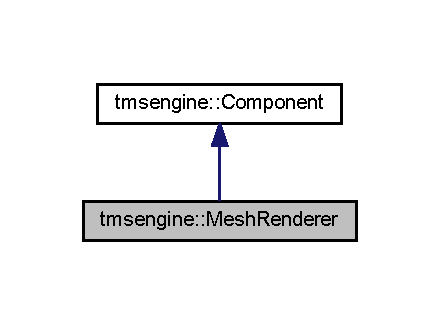
\includegraphics[width=211pt]{classtmsengine_1_1_mesh_renderer__inherit__graph}
\end{center}
\end{figure}


Collaboration diagram for tmsengine\+:\+:Mesh\+Renderer\+:\nopagebreak
\begin{figure}[H]
\begin{center}
\leavevmode
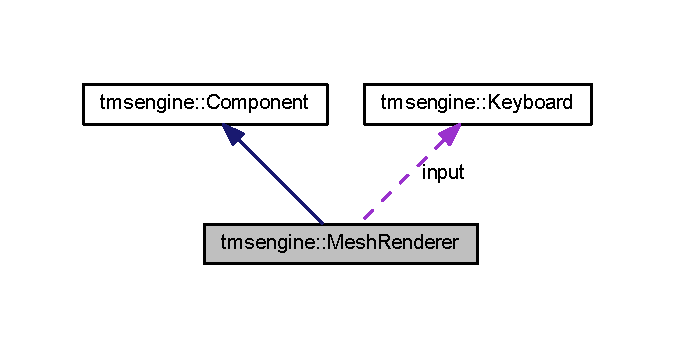
\includegraphics[width=324pt]{classtmsengine_1_1_mesh_renderer__coll__graph}
\end{center}
\end{figure}
\subsection*{Public Member Functions}
\begin{DoxyCompactItemize}
\item 
void \hyperlink{classtmsengine_1_1_mesh_renderer_a63ea3f394ba6678a6044068dd4253c97}{on\+Init} ()
\item 
void \hyperlink{classtmsengine_1_1_mesh_renderer_a1f1e2e0502438b6709e27a0b39c5ae9b}{set\+Mesh} (std\+::weak\+\_\+ptr$<$ \hyperlink{class_mesh}{Mesh} $>$ \hyperlink{classtmsengine_1_1_mesh_renderer_a6bc03b9b7e038a6e498fe7d54323d94e}{mesh})
\item 
std\+::shared\+\_\+ptr$<$ \hyperlink{class_mesh}{Mesh} $>$ \hyperlink{classtmsengine_1_1_mesh_renderer_a8f4724f163a3ff6e0eba9508380f79f1}{get\+Mesh} ()
\item 
std\+::shared\+\_\+ptr$<$ \hyperlink{class_material}{Material} $>$ \hyperlink{classtmsengine_1_1_mesh_renderer_a0d609c998a9c37b9282639432b165788}{get\+Material} ()
\end{DoxyCompactItemize}
\subsection*{Private Member Functions}
\begin{DoxyCompactItemize}
\item 
void \hyperlink{classtmsengine_1_1_mesh_renderer_adf77a2164ad1c92e4a310b99624b9fb5}{on\+Display} ()
\end{DoxyCompactItemize}
\subsection*{Private Attributes}
\begin{DoxyCompactItemize}
\item 
float \hyperlink{classtmsengine_1_1_mesh_renderer_aed43f36a26f4ab4fffad978f7efbcca1}{angle}
\item 
std\+::weak\+\_\+ptr$<$ \hyperlink{class_mesh}{Mesh} $>$ \hyperlink{classtmsengine_1_1_mesh_renderer_a6bc03b9b7e038a6e498fe7d54323d94e}{mesh}
\item 
std\+::shared\+\_\+ptr$<$ \hyperlink{class_material}{Material} $>$ \hyperlink{classtmsengine_1_1_mesh_renderer_ae9c9e481c73462163839fe0fccbc7de7}{material}
\item 
std\+::shared\+\_\+ptr$<$ \hyperlink{classtmsengine_1_1_vertex_array}{Vertex\+Array} $>$ \hyperlink{classtmsengine_1_1_mesh_renderer_a06a3739c8ec10c3e8beeea648701250a}{shape}
\item 
std\+::shared\+\_\+ptr$<$ \hyperlink{classtmsengine_1_1_shader_program}{Shader\+Program} $>$ \hyperlink{classtmsengine_1_1_mesh_renderer_aa303774109b5a5ca7c3ef0d10cea4508}{shader}
\item 
std\+::shared\+\_\+ptr$<$ \hyperlink{classtmsengine_1_1_vertex_array}{Vertex\+Array} $>$ \hyperlink{classtmsengine_1_1_mesh_renderer_aef537847320f1f0e6227f0e599f8b317}{hall\+Shape}
\item 
std\+::shared\+\_\+ptr$<$ \hyperlink{classtmsengine_1_1_texture}{Texture} $>$ \hyperlink{classtmsengine_1_1_mesh_renderer_adfb1c4c403365aaca511cce9c8533244}{hall\+Texture}
\item 
std\+::shared\+\_\+ptr$<$ \hyperlink{classtmsengine_1_1_vertex_array}{Vertex\+Array} $>$ \hyperlink{classtmsengine_1_1_mesh_renderer_a018cd9669b1d0fa770102fd9ec3c24e6}{object}
\item 
std\+::shared\+\_\+ptr$<$ \hyperlink{classtmsengine_1_1_texture}{Texture} $>$ \hyperlink{classtmsengine_1_1_mesh_renderer_aef2386e714dd2dfc616dc2249bc60d67}{texture}
\item 
\hyperlink{classtmsengine_1_1_keyboard}{Keyboard} \hyperlink{classtmsengine_1_1_mesh_renderer_a572d3dc4c4211c1d93645616b3ae26c7}{input}
\item 
glm\+::mat4 \hyperlink{classtmsengine_1_1_mesh_renderer_abac4546c1d1fa1144d88e0e11824b96a}{model}
\end{DoxyCompactItemize}


\subsection{Member Function Documentation}
\mbox{\Hypertarget{classtmsengine_1_1_mesh_renderer_a0d609c998a9c37b9282639432b165788}\label{classtmsengine_1_1_mesh_renderer_a0d609c998a9c37b9282639432b165788}} 
\index{tmsengine\+::\+Mesh\+Renderer@{tmsengine\+::\+Mesh\+Renderer}!get\+Material@{get\+Material}}
\index{get\+Material@{get\+Material}!tmsengine\+::\+Mesh\+Renderer@{tmsengine\+::\+Mesh\+Renderer}}
\subsubsection{\texorpdfstring{get\+Material()}{getMaterial()}}
{\footnotesize\ttfamily std\+::shared\+\_\+ptr$<$\hyperlink{class_material}{Material}$>$ tmsengine\+::\+Mesh\+Renderer\+::get\+Material (\begin{DoxyParamCaption}{ }\end{DoxyParamCaption})}

\mbox{\Hypertarget{classtmsengine_1_1_mesh_renderer_a8f4724f163a3ff6e0eba9508380f79f1}\label{classtmsengine_1_1_mesh_renderer_a8f4724f163a3ff6e0eba9508380f79f1}} 
\index{tmsengine\+::\+Mesh\+Renderer@{tmsengine\+::\+Mesh\+Renderer}!get\+Mesh@{get\+Mesh}}
\index{get\+Mesh@{get\+Mesh}!tmsengine\+::\+Mesh\+Renderer@{tmsengine\+::\+Mesh\+Renderer}}
\subsubsection{\texorpdfstring{get\+Mesh()}{getMesh()}}
{\footnotesize\ttfamily std\+::shared\+\_\+ptr$<$\hyperlink{class_mesh}{Mesh}$>$ tmsengine\+::\+Mesh\+Renderer\+::get\+Mesh (\begin{DoxyParamCaption}{ }\end{DoxyParamCaption})}

\mbox{\Hypertarget{classtmsengine_1_1_mesh_renderer_adf77a2164ad1c92e4a310b99624b9fb5}\label{classtmsengine_1_1_mesh_renderer_adf77a2164ad1c92e4a310b99624b9fb5}} 
\index{tmsengine\+::\+Mesh\+Renderer@{tmsengine\+::\+Mesh\+Renderer}!on\+Display@{on\+Display}}
\index{on\+Display@{on\+Display}!tmsengine\+::\+Mesh\+Renderer@{tmsengine\+::\+Mesh\+Renderer}}
\subsubsection{\texorpdfstring{on\+Display()}{onDisplay()}}
{\footnotesize\ttfamily void tmsengine\+::\+Mesh\+Renderer\+::on\+Display (\begin{DoxyParamCaption}{ }\end{DoxyParamCaption})\hspace{0.3cm}{\ttfamily [private]}, {\ttfamily [virtual]}}



Reimplemented from \hyperlink{classtmsengine_1_1_component_a73aa3564db299ef43100bd58d7cab65b}{tmsengine\+::\+Component}.

Here is the call graph for this function\+:\nopagebreak
\begin{figure}[H]
\begin{center}
\leavevmode
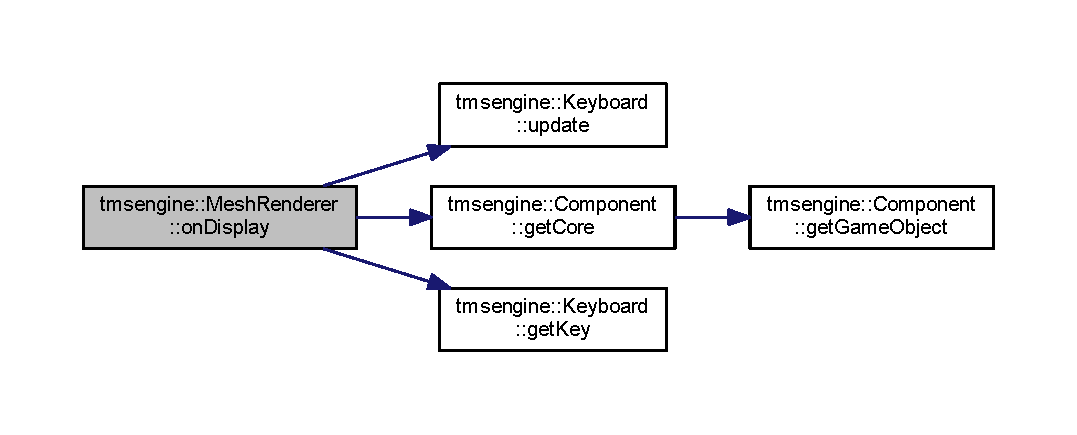
\includegraphics[width=350pt]{classtmsengine_1_1_mesh_renderer_adf77a2164ad1c92e4a310b99624b9fb5_cgraph}
\end{center}
\end{figure}
\mbox{\Hypertarget{classtmsengine_1_1_mesh_renderer_a63ea3f394ba6678a6044068dd4253c97}\label{classtmsengine_1_1_mesh_renderer_a63ea3f394ba6678a6044068dd4253c97}} 
\index{tmsengine\+::\+Mesh\+Renderer@{tmsengine\+::\+Mesh\+Renderer}!on\+Init@{on\+Init}}
\index{on\+Init@{on\+Init}!tmsengine\+::\+Mesh\+Renderer@{tmsengine\+::\+Mesh\+Renderer}}
\subsubsection{\texorpdfstring{on\+Init()}{onInit()}}
{\footnotesize\ttfamily void tmsengine\+::\+Mesh\+Renderer\+::on\+Init (\begin{DoxyParamCaption}{ }\end{DoxyParamCaption})\hspace{0.3cm}{\ttfamily [virtual]}}



Reimplemented from \hyperlink{classtmsengine_1_1_component_ae992e9b0c98b569eba13d0274089bc18}{tmsengine\+::\+Component}.

Here is the call graph for this function\+:\nopagebreak
\begin{figure}[H]
\begin{center}
\leavevmode
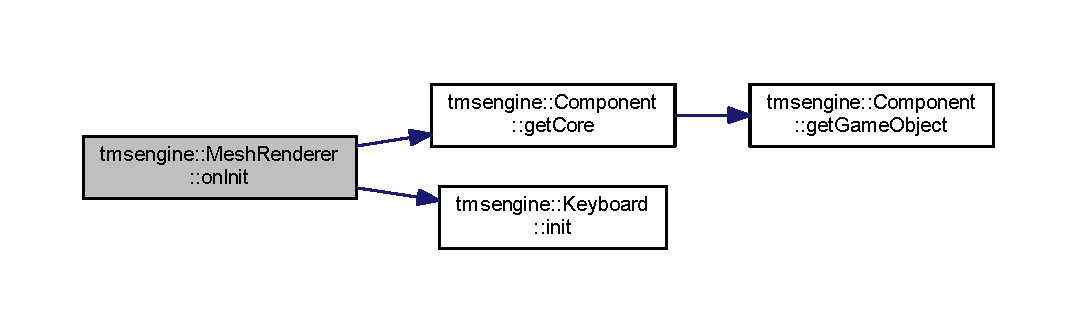
\includegraphics[width=350pt]{classtmsengine_1_1_mesh_renderer_a63ea3f394ba6678a6044068dd4253c97_cgraph}
\end{center}
\end{figure}
\mbox{\Hypertarget{classtmsengine_1_1_mesh_renderer_a1f1e2e0502438b6709e27a0b39c5ae9b}\label{classtmsengine_1_1_mesh_renderer_a1f1e2e0502438b6709e27a0b39c5ae9b}} 
\index{tmsengine\+::\+Mesh\+Renderer@{tmsengine\+::\+Mesh\+Renderer}!set\+Mesh@{set\+Mesh}}
\index{set\+Mesh@{set\+Mesh}!tmsengine\+::\+Mesh\+Renderer@{tmsengine\+::\+Mesh\+Renderer}}
\subsubsection{\texorpdfstring{set\+Mesh()}{setMesh()}}
{\footnotesize\ttfamily void tmsengine\+::\+Mesh\+Renderer\+::set\+Mesh (\begin{DoxyParamCaption}\item[{std\+::weak\+\_\+ptr$<$ \hyperlink{class_mesh}{Mesh} $>$}]{mesh }\end{DoxyParamCaption})}



\subsection{Member Data Documentation}
\mbox{\Hypertarget{classtmsengine_1_1_mesh_renderer_aed43f36a26f4ab4fffad978f7efbcca1}\label{classtmsengine_1_1_mesh_renderer_aed43f36a26f4ab4fffad978f7efbcca1}} 
\index{tmsengine\+::\+Mesh\+Renderer@{tmsengine\+::\+Mesh\+Renderer}!angle@{angle}}
\index{angle@{angle}!tmsengine\+::\+Mesh\+Renderer@{tmsengine\+::\+Mesh\+Renderer}}
\subsubsection{\texorpdfstring{angle}{angle}}
{\footnotesize\ttfamily float tmsengine\+::\+Mesh\+Renderer\+::angle\hspace{0.3cm}{\ttfamily [private]}}

\mbox{\Hypertarget{classtmsengine_1_1_mesh_renderer_aef537847320f1f0e6227f0e599f8b317}\label{classtmsengine_1_1_mesh_renderer_aef537847320f1f0e6227f0e599f8b317}} 
\index{tmsengine\+::\+Mesh\+Renderer@{tmsengine\+::\+Mesh\+Renderer}!hall\+Shape@{hall\+Shape}}
\index{hall\+Shape@{hall\+Shape}!tmsengine\+::\+Mesh\+Renderer@{tmsengine\+::\+Mesh\+Renderer}}
\subsubsection{\texorpdfstring{hall\+Shape}{hallShape}}
{\footnotesize\ttfamily std\+::shared\+\_\+ptr$<$\hyperlink{classtmsengine_1_1_vertex_array}{Vertex\+Array}$>$ tmsengine\+::\+Mesh\+Renderer\+::hall\+Shape\hspace{0.3cm}{\ttfamily [private]}}

\mbox{\Hypertarget{classtmsengine_1_1_mesh_renderer_adfb1c4c403365aaca511cce9c8533244}\label{classtmsengine_1_1_mesh_renderer_adfb1c4c403365aaca511cce9c8533244}} 
\index{tmsengine\+::\+Mesh\+Renderer@{tmsengine\+::\+Mesh\+Renderer}!hall\+Texture@{hall\+Texture}}
\index{hall\+Texture@{hall\+Texture}!tmsengine\+::\+Mesh\+Renderer@{tmsengine\+::\+Mesh\+Renderer}}
\subsubsection{\texorpdfstring{hall\+Texture}{hallTexture}}
{\footnotesize\ttfamily std\+::shared\+\_\+ptr$<$\hyperlink{classtmsengine_1_1_texture}{Texture}$>$ tmsengine\+::\+Mesh\+Renderer\+::hall\+Texture\hspace{0.3cm}{\ttfamily [private]}}

\mbox{\Hypertarget{classtmsengine_1_1_mesh_renderer_a572d3dc4c4211c1d93645616b3ae26c7}\label{classtmsengine_1_1_mesh_renderer_a572d3dc4c4211c1d93645616b3ae26c7}} 
\index{tmsengine\+::\+Mesh\+Renderer@{tmsengine\+::\+Mesh\+Renderer}!input@{input}}
\index{input@{input}!tmsengine\+::\+Mesh\+Renderer@{tmsengine\+::\+Mesh\+Renderer}}
\subsubsection{\texorpdfstring{input}{input}}
{\footnotesize\ttfamily \hyperlink{classtmsengine_1_1_keyboard}{Keyboard} tmsengine\+::\+Mesh\+Renderer\+::input\hspace{0.3cm}{\ttfamily [private]}}

\mbox{\Hypertarget{classtmsengine_1_1_mesh_renderer_ae9c9e481c73462163839fe0fccbc7de7}\label{classtmsengine_1_1_mesh_renderer_ae9c9e481c73462163839fe0fccbc7de7}} 
\index{tmsengine\+::\+Mesh\+Renderer@{tmsengine\+::\+Mesh\+Renderer}!material@{material}}
\index{material@{material}!tmsengine\+::\+Mesh\+Renderer@{tmsengine\+::\+Mesh\+Renderer}}
\subsubsection{\texorpdfstring{material}{material}}
{\footnotesize\ttfamily std\+::shared\+\_\+ptr$<$\hyperlink{class_material}{Material}$>$ tmsengine\+::\+Mesh\+Renderer\+::material\hspace{0.3cm}{\ttfamily [private]}}

\mbox{\Hypertarget{classtmsengine_1_1_mesh_renderer_a6bc03b9b7e038a6e498fe7d54323d94e}\label{classtmsengine_1_1_mesh_renderer_a6bc03b9b7e038a6e498fe7d54323d94e}} 
\index{tmsengine\+::\+Mesh\+Renderer@{tmsengine\+::\+Mesh\+Renderer}!mesh@{mesh}}
\index{mesh@{mesh}!tmsengine\+::\+Mesh\+Renderer@{tmsengine\+::\+Mesh\+Renderer}}
\subsubsection{\texorpdfstring{mesh}{mesh}}
{\footnotesize\ttfamily std\+::weak\+\_\+ptr$<$\hyperlink{class_mesh}{Mesh}$>$ tmsengine\+::\+Mesh\+Renderer\+::mesh\hspace{0.3cm}{\ttfamily [private]}}

\mbox{\Hypertarget{classtmsengine_1_1_mesh_renderer_abac4546c1d1fa1144d88e0e11824b96a}\label{classtmsengine_1_1_mesh_renderer_abac4546c1d1fa1144d88e0e11824b96a}} 
\index{tmsengine\+::\+Mesh\+Renderer@{tmsengine\+::\+Mesh\+Renderer}!model@{model}}
\index{model@{model}!tmsengine\+::\+Mesh\+Renderer@{tmsengine\+::\+Mesh\+Renderer}}
\subsubsection{\texorpdfstring{model}{model}}
{\footnotesize\ttfamily glm\+::mat4 tmsengine\+::\+Mesh\+Renderer\+::model\hspace{0.3cm}{\ttfamily [private]}}

\mbox{\Hypertarget{classtmsengine_1_1_mesh_renderer_a018cd9669b1d0fa770102fd9ec3c24e6}\label{classtmsengine_1_1_mesh_renderer_a018cd9669b1d0fa770102fd9ec3c24e6}} 
\index{tmsengine\+::\+Mesh\+Renderer@{tmsengine\+::\+Mesh\+Renderer}!object@{object}}
\index{object@{object}!tmsengine\+::\+Mesh\+Renderer@{tmsengine\+::\+Mesh\+Renderer}}
\subsubsection{\texorpdfstring{object}{object}}
{\footnotesize\ttfamily std\+::shared\+\_\+ptr$<$\hyperlink{classtmsengine_1_1_vertex_array}{Vertex\+Array}$>$ tmsengine\+::\+Mesh\+Renderer\+::object\hspace{0.3cm}{\ttfamily [private]}}

\mbox{\Hypertarget{classtmsengine_1_1_mesh_renderer_aa303774109b5a5ca7c3ef0d10cea4508}\label{classtmsengine_1_1_mesh_renderer_aa303774109b5a5ca7c3ef0d10cea4508}} 
\index{tmsengine\+::\+Mesh\+Renderer@{tmsengine\+::\+Mesh\+Renderer}!shader@{shader}}
\index{shader@{shader}!tmsengine\+::\+Mesh\+Renderer@{tmsengine\+::\+Mesh\+Renderer}}
\subsubsection{\texorpdfstring{shader}{shader}}
{\footnotesize\ttfamily std\+::shared\+\_\+ptr$<$\hyperlink{classtmsengine_1_1_shader_program}{Shader\+Program}$>$ tmsengine\+::\+Mesh\+Renderer\+::shader\hspace{0.3cm}{\ttfamily [private]}}

\mbox{\Hypertarget{classtmsengine_1_1_mesh_renderer_a06a3739c8ec10c3e8beeea648701250a}\label{classtmsengine_1_1_mesh_renderer_a06a3739c8ec10c3e8beeea648701250a}} 
\index{tmsengine\+::\+Mesh\+Renderer@{tmsengine\+::\+Mesh\+Renderer}!shape@{shape}}
\index{shape@{shape}!tmsengine\+::\+Mesh\+Renderer@{tmsengine\+::\+Mesh\+Renderer}}
\subsubsection{\texorpdfstring{shape}{shape}}
{\footnotesize\ttfamily std\+::shared\+\_\+ptr$<$\hyperlink{classtmsengine_1_1_vertex_array}{Vertex\+Array}$>$ tmsengine\+::\+Mesh\+Renderer\+::shape\hspace{0.3cm}{\ttfamily [private]}}

\mbox{\Hypertarget{classtmsengine_1_1_mesh_renderer_aef2386e714dd2dfc616dc2249bc60d67}\label{classtmsengine_1_1_mesh_renderer_aef2386e714dd2dfc616dc2249bc60d67}} 
\index{tmsengine\+::\+Mesh\+Renderer@{tmsengine\+::\+Mesh\+Renderer}!texture@{texture}}
\index{texture@{texture}!tmsengine\+::\+Mesh\+Renderer@{tmsengine\+::\+Mesh\+Renderer}}
\subsubsection{\texorpdfstring{texture}{texture}}
{\footnotesize\ttfamily std\+::shared\+\_\+ptr$<$\hyperlink{classtmsengine_1_1_texture}{Texture}$>$ tmsengine\+::\+Mesh\+Renderer\+::texture\hspace{0.3cm}{\ttfamily [private]}}



The documentation for this class was generated from the following files\+:\begin{DoxyCompactItemize}
\item 
T\+M\+S\+Engine/\hyperlink{_mesh_renderer_8h}{Mesh\+Renderer.\+h}\item 
T\+M\+S\+Engine/\hyperlink{_mesh_renderer_8cpp}{Mesh\+Renderer.\+cpp}\end{DoxyCompactItemize}

\hypertarget{class_resource}{}\section{Resource Class Reference}
\label{class_resource}\index{Resource@{Resource}}


{\ttfamily \#include $<$Resource.\+h$>$}

\subsection*{Private Attributes}
\begin{DoxyCompactItemize}
\item 
std\+::string \hyperlink{class_resource_a9d2af35bfd103fdc3f82a1bb8733a09d}{path}
\end{DoxyCompactItemize}


\subsection{Member Data Documentation}
\mbox{\Hypertarget{class_resource_a9d2af35bfd103fdc3f82a1bb8733a09d}\label{class_resource_a9d2af35bfd103fdc3f82a1bb8733a09d}} 
\index{Resource@{Resource}!path@{path}}
\index{path@{path}!Resource@{Resource}}
\subsubsection{\texorpdfstring{path}{path}}
{\footnotesize\ttfamily std\+::string Resource\+::path\hspace{0.3cm}{\ttfamily [private]}}



The documentation for this class was generated from the following file\+:\begin{DoxyCompactItemize}
\item 
T\+M\+S\+Engine/\+Resources/\hyperlink{_resource_8h}{Resource.\+h}\end{DoxyCompactItemize}

\hypertarget{class_resources}{}\section{Resources Class Reference}
\label{class_resources}\index{Resources@{Resources}}


{\ttfamily \#include $<$Resource\+Manager.\+h$>$}



The documentation for this class was generated from the following file\+:\begin{DoxyCompactItemize}
\item 
T\+M\+S\+Engine/\hyperlink{_resource_manager_8h}{Resource\+Manager.\+h}\end{DoxyCompactItemize}

\hypertarget{structtmsengine_1_1_sampler}{}\section{tmsengine\+:\+:Sampler Struct Reference}
\label{structtmsengine_1_1_sampler}\index{tmsengine\+::\+Sampler@{tmsengine\+::\+Sampler}}


{\ttfamily \#include $<$Shader\+Program.\+h$>$}

\subsection*{Public Attributes}
\begin{DoxyCompactItemize}
\item 
G\+Luint \hyperlink{structtmsengine_1_1_sampler_a565a09cf1484d33276993fd5c8eaec09}{sampler\+ID}
\item 
std\+::shared\+\_\+ptr$<$ \hyperlink{classtmsengine_1_1_texture}{Texture} $>$ \hyperlink{structtmsengine_1_1_sampler_af8ea8b2d52e4fd2bec956f844ebda8d9}{texture}
\end{DoxyCompactItemize}


\subsection{Member Data Documentation}
\mbox{\Hypertarget{structtmsengine_1_1_sampler_a565a09cf1484d33276993fd5c8eaec09}\label{structtmsengine_1_1_sampler_a565a09cf1484d33276993fd5c8eaec09}} 
\index{tmsengine\+::\+Sampler@{tmsengine\+::\+Sampler}!sampler\+ID@{sampler\+ID}}
\index{sampler\+ID@{sampler\+ID}!tmsengine\+::\+Sampler@{tmsengine\+::\+Sampler}}
\subsubsection{\texorpdfstring{sampler\+ID}{samplerID}}
{\footnotesize\ttfamily G\+Luint tmsengine\+::\+Sampler\+::sampler\+ID}

\mbox{\Hypertarget{structtmsengine_1_1_sampler_af8ea8b2d52e4fd2bec956f844ebda8d9}\label{structtmsengine_1_1_sampler_af8ea8b2d52e4fd2bec956f844ebda8d9}} 
\index{tmsengine\+::\+Sampler@{tmsengine\+::\+Sampler}!texture@{texture}}
\index{texture@{texture}!tmsengine\+::\+Sampler@{tmsengine\+::\+Sampler}}
\subsubsection{\texorpdfstring{texture}{texture}}
{\footnotesize\ttfamily std\+::shared\+\_\+ptr$<$\hyperlink{classtmsengine_1_1_texture}{Texture}$>$ tmsengine\+::\+Sampler\+::texture}



The documentation for this struct was generated from the following file\+:\begin{DoxyCompactItemize}
\item 
T\+M\+S\+Engine/\hyperlink{_shader_program_8h}{Shader\+Program.\+h}\end{DoxyCompactItemize}

\hypertarget{classtmsengine_1_1_screen}{}\section{tmsengine\+:\+:Screen Class Reference}
\label{classtmsengine_1_1_screen}\index{tmsengine\+::\+Screen@{tmsengine\+::\+Screen}}


{\ttfamily \#include $<$Screen.\+h$>$}

\subsection*{Public Member Functions}
\begin{DoxyCompactItemize}
\item 
void \hyperlink{classtmsengine_1_1_screen_a532300498d439e91852b1c400bc5548a}{Screen\+Init} ()
\item 
void \hyperlink{classtmsengine_1_1_screen_ab662ffd34dd93ef78adc63a3bfc6db18}{Clear\+Buff} ()
\item 
void \hyperlink{classtmsengine_1_1_screen_af9c6d28da2a6008de16c358321aa12ab}{Swap\+Screen} ()
\item 
S\+D\+L\+\_\+\+Window $\ast$ \hyperlink{classtmsengine_1_1_screen_acda07bc9c3c4dbff93b9a5c52a1a26b2}{Get\+Screen} ()
\end{DoxyCompactItemize}
\subsection*{Static Public Member Functions}
\begin{DoxyCompactItemize}
\item 
static int \hyperlink{classtmsengine_1_1_screen_a705d20e6bdc79d8a176cffee3f4de363}{get\+Width} ()
\item 
static int \hyperlink{classtmsengine_1_1_screen_a0192fc98efb3fb523858082312fbe1a7}{get\+Height} ()
\end{DoxyCompactItemize}
\subsection*{Private Attributes}
\begin{DoxyCompactItemize}
\item 
S\+D\+L\+\_\+\+Window $\ast$ \hyperlink{classtmsengine_1_1_screen_a0fa3ebd5ed7a46a76312f09623a447f3}{window}
\end{DoxyCompactItemize}
\subsection*{Static Private Attributes}
\begin{DoxyCompactItemize}
\item 
static int \hyperlink{classtmsengine_1_1_screen_afa7a1938c25c1e724b698a9aa6dcc9b1}{win\+PosX} = 100
\item 
static int \hyperlink{classtmsengine_1_1_screen_aafa7ecb9c6daa3733662228ed92d388e}{win\+PosY} = 100
\item 
static int \hyperlink{classtmsengine_1_1_screen_a2ed0e8d3a57009e961f391b2b4993b3b}{win\+Width} = 500
\item 
static int \hyperlink{classtmsengine_1_1_screen_a3a62139bebecea188873b9b30122a6ec}{win\+Height} = 500
\end{DoxyCompactItemize}


\subsection{Member Function Documentation}
\mbox{\Hypertarget{classtmsengine_1_1_screen_ab662ffd34dd93ef78adc63a3bfc6db18}\label{classtmsengine_1_1_screen_ab662ffd34dd93ef78adc63a3bfc6db18}} 
\index{tmsengine\+::\+Screen@{tmsengine\+::\+Screen}!Clear\+Buff@{Clear\+Buff}}
\index{Clear\+Buff@{Clear\+Buff}!tmsengine\+::\+Screen@{tmsengine\+::\+Screen}}
\subsubsection{\texorpdfstring{Clear\+Buff()}{ClearBuff()}}
{\footnotesize\ttfamily void tmsengine\+::\+Screen\+::\+Clear\+Buff (\begin{DoxyParamCaption}{ }\end{DoxyParamCaption})}

Here is the caller graph for this function\+:\nopagebreak
\begin{figure}[H]
\begin{center}
\leavevmode
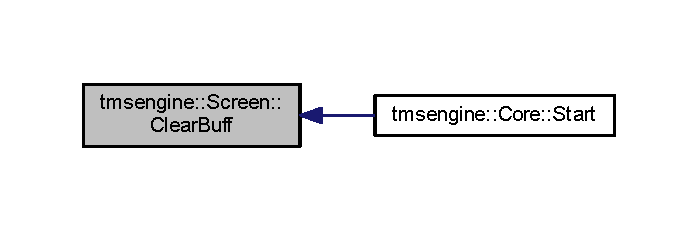
\includegraphics[width=335pt]{classtmsengine_1_1_screen_ab662ffd34dd93ef78adc63a3bfc6db18_icgraph}
\end{center}
\end{figure}
\mbox{\Hypertarget{classtmsengine_1_1_screen_a0192fc98efb3fb523858082312fbe1a7}\label{classtmsengine_1_1_screen_a0192fc98efb3fb523858082312fbe1a7}} 
\index{tmsengine\+::\+Screen@{tmsengine\+::\+Screen}!get\+Height@{get\+Height}}
\index{get\+Height@{get\+Height}!tmsengine\+::\+Screen@{tmsengine\+::\+Screen}}
\subsubsection{\texorpdfstring{get\+Height()}{getHeight()}}
{\footnotesize\ttfamily int tmsengine\+::\+Screen\+::get\+Height (\begin{DoxyParamCaption}{ }\end{DoxyParamCaption})\hspace{0.3cm}{\ttfamily [static]}}

\mbox{\Hypertarget{classtmsengine_1_1_screen_acda07bc9c3c4dbff93b9a5c52a1a26b2}\label{classtmsengine_1_1_screen_acda07bc9c3c4dbff93b9a5c52a1a26b2}} 
\index{tmsengine\+::\+Screen@{tmsengine\+::\+Screen}!Get\+Screen@{Get\+Screen}}
\index{Get\+Screen@{Get\+Screen}!tmsengine\+::\+Screen@{tmsengine\+::\+Screen}}
\subsubsection{\texorpdfstring{Get\+Screen()}{GetScreen()}}
{\footnotesize\ttfamily S\+D\+L\+\_\+\+Window $\ast$ tmsengine\+::\+Screen\+::\+Get\+Screen (\begin{DoxyParamCaption}{ }\end{DoxyParamCaption})}

\mbox{\Hypertarget{classtmsengine_1_1_screen_a705d20e6bdc79d8a176cffee3f4de363}\label{classtmsengine_1_1_screen_a705d20e6bdc79d8a176cffee3f4de363}} 
\index{tmsengine\+::\+Screen@{tmsengine\+::\+Screen}!get\+Width@{get\+Width}}
\index{get\+Width@{get\+Width}!tmsengine\+::\+Screen@{tmsengine\+::\+Screen}}
\subsubsection{\texorpdfstring{get\+Width()}{getWidth()}}
{\footnotesize\ttfamily int tmsengine\+::\+Screen\+::get\+Width (\begin{DoxyParamCaption}{ }\end{DoxyParamCaption})\hspace{0.3cm}{\ttfamily [static]}}

\mbox{\Hypertarget{classtmsengine_1_1_screen_a532300498d439e91852b1c400bc5548a}\label{classtmsengine_1_1_screen_a532300498d439e91852b1c400bc5548a}} 
\index{tmsengine\+::\+Screen@{tmsengine\+::\+Screen}!Screen\+Init@{Screen\+Init}}
\index{Screen\+Init@{Screen\+Init}!tmsengine\+::\+Screen@{tmsengine\+::\+Screen}}
\subsubsection{\texorpdfstring{Screen\+Init()}{ScreenInit()}}
{\footnotesize\ttfamily void tmsengine\+::\+Screen\+::\+Screen\+Init (\begin{DoxyParamCaption}{ }\end{DoxyParamCaption})}

\mbox{\Hypertarget{classtmsengine_1_1_screen_af9c6d28da2a6008de16c358321aa12ab}\label{classtmsengine_1_1_screen_af9c6d28da2a6008de16c358321aa12ab}} 
\index{tmsengine\+::\+Screen@{tmsengine\+::\+Screen}!Swap\+Screen@{Swap\+Screen}}
\index{Swap\+Screen@{Swap\+Screen}!tmsengine\+::\+Screen@{tmsengine\+::\+Screen}}
\subsubsection{\texorpdfstring{Swap\+Screen()}{SwapScreen()}}
{\footnotesize\ttfamily void tmsengine\+::\+Screen\+::\+Swap\+Screen (\begin{DoxyParamCaption}{ }\end{DoxyParamCaption})}

Here is the caller graph for this function\+:\nopagebreak
\begin{figure}[H]
\begin{center}
\leavevmode
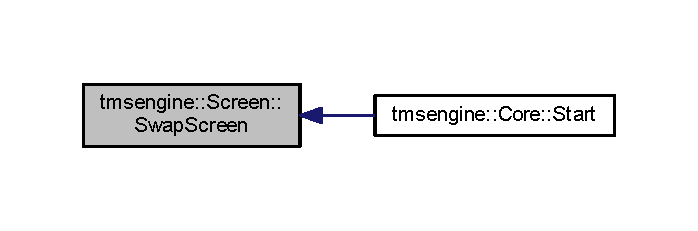
\includegraphics[width=335pt]{classtmsengine_1_1_screen_af9c6d28da2a6008de16c358321aa12ab_icgraph}
\end{center}
\end{figure}


\subsection{Member Data Documentation}
\mbox{\Hypertarget{classtmsengine_1_1_screen_a0fa3ebd5ed7a46a76312f09623a447f3}\label{classtmsengine_1_1_screen_a0fa3ebd5ed7a46a76312f09623a447f3}} 
\index{tmsengine\+::\+Screen@{tmsengine\+::\+Screen}!window@{window}}
\index{window@{window}!tmsengine\+::\+Screen@{tmsengine\+::\+Screen}}
\subsubsection{\texorpdfstring{window}{window}}
{\footnotesize\ttfamily S\+D\+L\+\_\+\+Window$\ast$ tmsengine\+::\+Screen\+::window\hspace{0.3cm}{\ttfamily [private]}}

\mbox{\Hypertarget{classtmsengine_1_1_screen_a3a62139bebecea188873b9b30122a6ec}\label{classtmsengine_1_1_screen_a3a62139bebecea188873b9b30122a6ec}} 
\index{tmsengine\+::\+Screen@{tmsengine\+::\+Screen}!win\+Height@{win\+Height}}
\index{win\+Height@{win\+Height}!tmsengine\+::\+Screen@{tmsengine\+::\+Screen}}
\subsubsection{\texorpdfstring{win\+Height}{winHeight}}
{\footnotesize\ttfamily int tmsengine\+::\+Screen\+::win\+Height = 500\hspace{0.3cm}{\ttfamily [static]}, {\ttfamily [private]}}

\mbox{\Hypertarget{classtmsengine_1_1_screen_afa7a1938c25c1e724b698a9aa6dcc9b1}\label{classtmsengine_1_1_screen_afa7a1938c25c1e724b698a9aa6dcc9b1}} 
\index{tmsengine\+::\+Screen@{tmsengine\+::\+Screen}!win\+PosX@{win\+PosX}}
\index{win\+PosX@{win\+PosX}!tmsengine\+::\+Screen@{tmsengine\+::\+Screen}}
\subsubsection{\texorpdfstring{win\+PosX}{winPosX}}
{\footnotesize\ttfamily int tmsengine\+::\+Screen\+::win\+PosX = 100\hspace{0.3cm}{\ttfamily [static]}, {\ttfamily [private]}}

\mbox{\Hypertarget{classtmsengine_1_1_screen_aafa7ecb9c6daa3733662228ed92d388e}\label{classtmsengine_1_1_screen_aafa7ecb9c6daa3733662228ed92d388e}} 
\index{tmsengine\+::\+Screen@{tmsengine\+::\+Screen}!win\+PosY@{win\+PosY}}
\index{win\+PosY@{win\+PosY}!tmsengine\+::\+Screen@{tmsengine\+::\+Screen}}
\subsubsection{\texorpdfstring{win\+PosY}{winPosY}}
{\footnotesize\ttfamily int tmsengine\+::\+Screen\+::win\+PosY = 100\hspace{0.3cm}{\ttfamily [static]}, {\ttfamily [private]}}

\mbox{\Hypertarget{classtmsengine_1_1_screen_a2ed0e8d3a57009e961f391b2b4993b3b}\label{classtmsengine_1_1_screen_a2ed0e8d3a57009e961f391b2b4993b3b}} 
\index{tmsengine\+::\+Screen@{tmsengine\+::\+Screen}!win\+Width@{win\+Width}}
\index{win\+Width@{win\+Width}!tmsengine\+::\+Screen@{tmsengine\+::\+Screen}}
\subsubsection{\texorpdfstring{win\+Width}{winWidth}}
{\footnotesize\ttfamily int tmsengine\+::\+Screen\+::win\+Width = 500\hspace{0.3cm}{\ttfamily [static]}, {\ttfamily [private]}}



The documentation for this class was generated from the following files\+:\begin{DoxyCompactItemize}
\item 
T\+M\+S\+Engine/\hyperlink{_screen_8h}{Screen.\+h}\item 
T\+M\+S\+Engine/\hyperlink{_screen_8cpp}{Screen.\+cpp}\end{DoxyCompactItemize}

\hypertarget{class_shader}{}\section{Shader Class Reference}
\label{class_shader}\index{Shader@{Shader}}


{\ttfamily \#include $<$Shader.\+h$>$}

\subsection*{Public Member Functions}
\begin{DoxyCompactItemize}
\item 
\hyperlink{class_shader_aff01df87e8a102f270b5b135a295e59d}{$\sim$\+Shader} ()
\item 
void \hyperlink{class_shader_a6826cb5394def93884540565ffa4df7d}{set\+Uniform} (std\+::string name, float value)
\item 
void \hyperlink{class_shader_a94dca1a3185ca11e8e0ca7f77c3ecb34}{set\+Uniform} (std\+::string name, std\+::weak\+\_\+ptr$<$ Texture $>$ value)
\item 
void \hyperlink{class_shader_a3f94c37778540d4d0d7ff107936e3750}{set\+Uniform} (std\+::string name, glm\+::mat4 value)
\item 
void \hyperlink{class_shader_ad97eff9ea48cee42227e31c56cd7479e}{set\+Uniform} (std\+::string name, glm\+::vec3 value)
\item 
G\+Luint \hyperlink{class_shader_ad1bc9a16400499ec80c4f716a390abaf}{get\+ID} ()
\end{DoxyCompactItemize}
\subsection*{Private Member Functions}
\begin{DoxyCompactItemize}
\item 
std\+::shared\+\_\+ptr$<$ \hyperlink{class_shader}{Shader} $>$ \hyperlink{class_shader_af67abb9216bbd4729181ed6cf8260baf}{create} (std\+::string vert\+Src, std\+::string frag\+Src)
\item 
std\+::shared\+\_\+ptr$<$ \hyperlink{class_shader}{Shader} $>$ \hyperlink{class_shader_ab80e1350b80a6f6ccc3e28aca8ca3536}{load} (std\+::string path)
\end{DoxyCompactItemize}


\subsection{Constructor \& Destructor Documentation}
\mbox{\Hypertarget{class_shader_aff01df87e8a102f270b5b135a295e59d}\label{class_shader_aff01df87e8a102f270b5b135a295e59d}} 
\index{Shader@{Shader}!````~Shader@{$\sim$\+Shader}}
\index{````~Shader@{$\sim$\+Shader}!Shader@{Shader}}
\subsubsection{\texorpdfstring{$\sim$\+Shader()}{~Shader()}}
{\footnotesize\ttfamily Shader\+::$\sim$\+Shader (\begin{DoxyParamCaption}{ }\end{DoxyParamCaption})}



\subsection{Member Function Documentation}
\mbox{\Hypertarget{class_shader_af67abb9216bbd4729181ed6cf8260baf}\label{class_shader_af67abb9216bbd4729181ed6cf8260baf}} 
\index{Shader@{Shader}!create@{create}}
\index{create@{create}!Shader@{Shader}}
\subsubsection{\texorpdfstring{create()}{create()}}
{\footnotesize\ttfamily std\+::shared\+\_\+ptr$<$\hyperlink{class_shader}{Shader}$>$ Shader\+::create (\begin{DoxyParamCaption}\item[{std\+::string}]{vert\+Src,  }\item[{std\+::string}]{frag\+Src }\end{DoxyParamCaption})\hspace{0.3cm}{\ttfamily [private]}}

\mbox{\Hypertarget{class_shader_ad1bc9a16400499ec80c4f716a390abaf}\label{class_shader_ad1bc9a16400499ec80c4f716a390abaf}} 
\index{Shader@{Shader}!get\+ID@{get\+ID}}
\index{get\+ID@{get\+ID}!Shader@{Shader}}
\subsubsection{\texorpdfstring{get\+I\+D()}{getID()}}
{\footnotesize\ttfamily G\+Luint Shader\+::get\+ID (\begin{DoxyParamCaption}{ }\end{DoxyParamCaption})}

\mbox{\Hypertarget{class_shader_ab80e1350b80a6f6ccc3e28aca8ca3536}\label{class_shader_ab80e1350b80a6f6ccc3e28aca8ca3536}} 
\index{Shader@{Shader}!load@{load}}
\index{load@{load}!Shader@{Shader}}
\subsubsection{\texorpdfstring{load()}{load()}}
{\footnotesize\ttfamily std\+::shared\+\_\+ptr$<$\hyperlink{class_shader}{Shader}$>$ Shader\+::load (\begin{DoxyParamCaption}\item[{std\+::string}]{path }\end{DoxyParamCaption})\hspace{0.3cm}{\ttfamily [private]}}

\mbox{\Hypertarget{class_shader_a6826cb5394def93884540565ffa4df7d}\label{class_shader_a6826cb5394def93884540565ffa4df7d}} 
\index{Shader@{Shader}!set\+Uniform@{set\+Uniform}}
\index{set\+Uniform@{set\+Uniform}!Shader@{Shader}}
\subsubsection{\texorpdfstring{set\+Uniform()}{setUniform()}\hspace{0.1cm}{\footnotesize\ttfamily [1/4]}}
{\footnotesize\ttfamily void Shader\+::set\+Uniform (\begin{DoxyParamCaption}\item[{std\+::string}]{name,  }\item[{float}]{value }\end{DoxyParamCaption})}

\mbox{\Hypertarget{class_shader_a94dca1a3185ca11e8e0ca7f77c3ecb34}\label{class_shader_a94dca1a3185ca11e8e0ca7f77c3ecb34}} 
\index{Shader@{Shader}!set\+Uniform@{set\+Uniform}}
\index{set\+Uniform@{set\+Uniform}!Shader@{Shader}}
\subsubsection{\texorpdfstring{set\+Uniform()}{setUniform()}\hspace{0.1cm}{\footnotesize\ttfamily [2/4]}}
{\footnotesize\ttfamily void Shader\+::set\+Uniform (\begin{DoxyParamCaption}\item[{std\+::string}]{name,  }\item[{std\+::weak\+\_\+ptr$<$ Texture $>$}]{value }\end{DoxyParamCaption})}

\mbox{\Hypertarget{class_shader_a3f94c37778540d4d0d7ff107936e3750}\label{class_shader_a3f94c37778540d4d0d7ff107936e3750}} 
\index{Shader@{Shader}!set\+Uniform@{set\+Uniform}}
\index{set\+Uniform@{set\+Uniform}!Shader@{Shader}}
\subsubsection{\texorpdfstring{set\+Uniform()}{setUniform()}\hspace{0.1cm}{\footnotesize\ttfamily [3/4]}}
{\footnotesize\ttfamily void Shader\+::set\+Uniform (\begin{DoxyParamCaption}\item[{std\+::string}]{name,  }\item[{glm\+::mat4}]{value }\end{DoxyParamCaption})}

\mbox{\Hypertarget{class_shader_ad97eff9ea48cee42227e31c56cd7479e}\label{class_shader_ad97eff9ea48cee42227e31c56cd7479e}} 
\index{Shader@{Shader}!set\+Uniform@{set\+Uniform}}
\index{set\+Uniform@{set\+Uniform}!Shader@{Shader}}
\subsubsection{\texorpdfstring{set\+Uniform()}{setUniform()}\hspace{0.1cm}{\footnotesize\ttfamily [4/4]}}
{\footnotesize\ttfamily void Shader\+::set\+Uniform (\begin{DoxyParamCaption}\item[{std\+::string}]{name,  }\item[{glm\+::vec3}]{value }\end{DoxyParamCaption})}



The documentation for this class was generated from the following file\+:\begin{DoxyCompactItemize}
\item 
T\+M\+S\+Engine/\+Resources/\hyperlink{_shader_8h}{Shader.\+h}\end{DoxyCompactItemize}

\hypertarget{classtmsengine_1_1_shader_program}{}\section{tmsengine\+:\+:Shader\+Program Class Reference}
\label{classtmsengine_1_1_shader_program}\index{tmsengine\+::\+Shader\+Program@{tmsengine\+::\+Shader\+Program}}


{\ttfamily \#include $<$Shader\+Program.\+h$>$}

\subsection*{Public Member Functions}
\begin{DoxyCompactItemize}
\item 
\hyperlink{classtmsengine_1_1_shader_program_abb515227032a61eef897c233ca5112d7}{Shader\+Program} (std\+::string vert, std\+::string frag)
\item 
void \hyperlink{classtmsengine_1_1_shader_program_a3508cadd306f94e631c68482e823bcc0}{draw} (std\+::shared\+\_\+ptr$<$ \hyperlink{classtmsengine_1_1_vertex_array}{Vertex\+Array} $>$ vertex\+Array)
\item 
void \hyperlink{classtmsengine_1_1_shader_program_a0c21d10770fc6753a33ebc2523b2a11d}{set\+Uniform} (std\+::string uniform, glm\+::vec4 value)
\item 
void \hyperlink{classtmsengine_1_1_shader_program_a18107f338613062ed17b0fd029437a81}{set\+Uniform} (std\+::string uniform, float value)
\item 
void \hyperlink{classtmsengine_1_1_shader_program_a5adad298f4eb24e342c0fa5b79dd90a6}{set\+Uniform} (std\+::string uniform, glm\+::mat4 value)
\item 
void \hyperlink{classtmsengine_1_1_shader_program_a048ea3e952f3a2480f20d2b521b56743}{set\+Uniform} (std\+::string uniform, std\+::shared\+\_\+ptr$<$ \hyperlink{classtmsengine_1_1_texture}{Texture} $>$ texture)
\item 
G\+Luint \hyperlink{classtmsengine_1_1_shader_program_a370a695c250cdf490ef8c8573701afed}{get\+ID} ()
\end{DoxyCompactItemize}
\subsection*{Private Attributes}
\begin{DoxyCompactItemize}
\item 
G\+Luint \hyperlink{classtmsengine_1_1_shader_program_a23f13b0cc16d56fd9d1423e06442d67c}{program\+ID}
\item 
std\+::vector$<$ \hyperlink{structtmsengine_1_1_sampler}{Sampler} $>$ \hyperlink{classtmsengine_1_1_shader_program_a3f32e04874a593207c3e2fe5aaef2e5e}{samplers}
\end{DoxyCompactItemize}


\subsection{Constructor \& Destructor Documentation}
\mbox{\Hypertarget{classtmsengine_1_1_shader_program_abb515227032a61eef897c233ca5112d7}\label{classtmsengine_1_1_shader_program_abb515227032a61eef897c233ca5112d7}} 
\index{tmsengine\+::\+Shader\+Program@{tmsengine\+::\+Shader\+Program}!Shader\+Program@{Shader\+Program}}
\index{Shader\+Program@{Shader\+Program}!tmsengine\+::\+Shader\+Program@{tmsengine\+::\+Shader\+Program}}
\subsubsection{\texorpdfstring{Shader\+Program()}{ShaderProgram()}}
{\footnotesize\ttfamily Shader\+Program\+::\+Shader\+Program (\begin{DoxyParamCaption}\item[{std\+::string}]{vert,  }\item[{std\+::string}]{frag }\end{DoxyParamCaption})}



\subsection{Member Function Documentation}
\mbox{\Hypertarget{classtmsengine_1_1_shader_program_a3508cadd306f94e631c68482e823bcc0}\label{classtmsengine_1_1_shader_program_a3508cadd306f94e631c68482e823bcc0}} 
\index{tmsengine\+::\+Shader\+Program@{tmsengine\+::\+Shader\+Program}!draw@{draw}}
\index{draw@{draw}!tmsengine\+::\+Shader\+Program@{tmsengine\+::\+Shader\+Program}}
\subsubsection{\texorpdfstring{draw()}{draw()}}
{\footnotesize\ttfamily void Shader\+Program\+::draw (\begin{DoxyParamCaption}\item[{std\+::shared\+\_\+ptr$<$ \hyperlink{classtmsengine_1_1_vertex_array}{Vertex\+Array} $>$}]{vertex\+Array }\end{DoxyParamCaption})}

\mbox{\Hypertarget{classtmsengine_1_1_shader_program_a370a695c250cdf490ef8c8573701afed}\label{classtmsengine_1_1_shader_program_a370a695c250cdf490ef8c8573701afed}} 
\index{tmsengine\+::\+Shader\+Program@{tmsengine\+::\+Shader\+Program}!get\+ID@{get\+ID}}
\index{get\+ID@{get\+ID}!tmsengine\+::\+Shader\+Program@{tmsengine\+::\+Shader\+Program}}
\subsubsection{\texorpdfstring{get\+I\+D()}{getID()}}
{\footnotesize\ttfamily G\+Luint Shader\+Program\+::get\+ID (\begin{DoxyParamCaption}{ }\end{DoxyParamCaption})}

\mbox{\Hypertarget{classtmsengine_1_1_shader_program_a0c21d10770fc6753a33ebc2523b2a11d}\label{classtmsengine_1_1_shader_program_a0c21d10770fc6753a33ebc2523b2a11d}} 
\index{tmsengine\+::\+Shader\+Program@{tmsengine\+::\+Shader\+Program}!set\+Uniform@{set\+Uniform}}
\index{set\+Uniform@{set\+Uniform}!tmsengine\+::\+Shader\+Program@{tmsengine\+::\+Shader\+Program}}
\subsubsection{\texorpdfstring{set\+Uniform()}{setUniform()}\hspace{0.1cm}{\footnotesize\ttfamily [1/4]}}
{\footnotesize\ttfamily void Shader\+Program\+::set\+Uniform (\begin{DoxyParamCaption}\item[{std\+::string}]{uniform,  }\item[{glm\+::vec4}]{value }\end{DoxyParamCaption})}

\mbox{\Hypertarget{classtmsengine_1_1_shader_program_a18107f338613062ed17b0fd029437a81}\label{classtmsengine_1_1_shader_program_a18107f338613062ed17b0fd029437a81}} 
\index{tmsengine\+::\+Shader\+Program@{tmsengine\+::\+Shader\+Program}!set\+Uniform@{set\+Uniform}}
\index{set\+Uniform@{set\+Uniform}!tmsengine\+::\+Shader\+Program@{tmsengine\+::\+Shader\+Program}}
\subsubsection{\texorpdfstring{set\+Uniform()}{setUniform()}\hspace{0.1cm}{\footnotesize\ttfamily [2/4]}}
{\footnotesize\ttfamily void Shader\+Program\+::set\+Uniform (\begin{DoxyParamCaption}\item[{std\+::string}]{uniform,  }\item[{float}]{value }\end{DoxyParamCaption})}

\mbox{\Hypertarget{classtmsengine_1_1_shader_program_a5adad298f4eb24e342c0fa5b79dd90a6}\label{classtmsengine_1_1_shader_program_a5adad298f4eb24e342c0fa5b79dd90a6}} 
\index{tmsengine\+::\+Shader\+Program@{tmsengine\+::\+Shader\+Program}!set\+Uniform@{set\+Uniform}}
\index{set\+Uniform@{set\+Uniform}!tmsengine\+::\+Shader\+Program@{tmsengine\+::\+Shader\+Program}}
\subsubsection{\texorpdfstring{set\+Uniform()}{setUniform()}\hspace{0.1cm}{\footnotesize\ttfamily [3/4]}}
{\footnotesize\ttfamily void Shader\+Program\+::set\+Uniform (\begin{DoxyParamCaption}\item[{std\+::string}]{uniform,  }\item[{glm\+::mat4}]{value }\end{DoxyParamCaption})}

\mbox{\Hypertarget{classtmsengine_1_1_shader_program_a048ea3e952f3a2480f20d2b521b56743}\label{classtmsengine_1_1_shader_program_a048ea3e952f3a2480f20d2b521b56743}} 
\index{tmsengine\+::\+Shader\+Program@{tmsengine\+::\+Shader\+Program}!set\+Uniform@{set\+Uniform}}
\index{set\+Uniform@{set\+Uniform}!tmsengine\+::\+Shader\+Program@{tmsengine\+::\+Shader\+Program}}
\subsubsection{\texorpdfstring{set\+Uniform()}{setUniform()}\hspace{0.1cm}{\footnotesize\ttfamily [4/4]}}
{\footnotesize\ttfamily void Shader\+Program\+::set\+Uniform (\begin{DoxyParamCaption}\item[{std\+::string}]{uniform,  }\item[{std\+::shared\+\_\+ptr$<$ \hyperlink{classtmsengine_1_1_texture}{Texture} $>$}]{texture }\end{DoxyParamCaption})}



\subsection{Member Data Documentation}
\mbox{\Hypertarget{classtmsengine_1_1_shader_program_a23f13b0cc16d56fd9d1423e06442d67c}\label{classtmsengine_1_1_shader_program_a23f13b0cc16d56fd9d1423e06442d67c}} 
\index{tmsengine\+::\+Shader\+Program@{tmsengine\+::\+Shader\+Program}!program\+ID@{program\+ID}}
\index{program\+ID@{program\+ID}!tmsengine\+::\+Shader\+Program@{tmsengine\+::\+Shader\+Program}}
\subsubsection{\texorpdfstring{program\+ID}{programID}}
{\footnotesize\ttfamily G\+Luint tmsengine\+::\+Shader\+Program\+::program\+ID\hspace{0.3cm}{\ttfamily [private]}}

\mbox{\Hypertarget{classtmsengine_1_1_shader_program_a3f32e04874a593207c3e2fe5aaef2e5e}\label{classtmsengine_1_1_shader_program_a3f32e04874a593207c3e2fe5aaef2e5e}} 
\index{tmsengine\+::\+Shader\+Program@{tmsengine\+::\+Shader\+Program}!samplers@{samplers}}
\index{samplers@{samplers}!tmsengine\+::\+Shader\+Program@{tmsengine\+::\+Shader\+Program}}
\subsubsection{\texorpdfstring{samplers}{samplers}}
{\footnotesize\ttfamily std\+::vector$<$\hyperlink{structtmsengine_1_1_sampler}{Sampler}$>$ tmsengine\+::\+Shader\+Program\+::samplers\hspace{0.3cm}{\ttfamily [private]}}



The documentation for this class was generated from the following files\+:\begin{DoxyCompactItemize}
\item 
T\+M\+S\+Engine/\hyperlink{_shader_program_8h}{Shader\+Program.\+h}\item 
T\+M\+S\+Engine/\hyperlink{_shader_program_8cpp}{Shader\+Program.\+cpp}\end{DoxyCompactItemize}

\hypertarget{classtmsengine_1_1_sound}{}\section{tmsengine\+:\+:Sound Class Reference}
\label{classtmsengine_1_1_sound}\index{tmsengine\+::\+Sound@{tmsengine\+::\+Sound}}


{\ttfamily \#include $<$Sound.\+h$>$}

\subsection*{Public Member Functions}
\begin{DoxyCompactItemize}
\item 
\hyperlink{classtmsengine_1_1_sound_a0da875f18794380a2f8a6e9d02e9d0cd}{Sound} ()
\item 
\hyperlink{classtmsengine_1_1_sound_a666456cd06cec8089d5be3fce56132f1}{Sound} (std\+::string path)
\item 
void \hyperlink{classtmsengine_1_1_sound_aca383fe0b166a15eae25580e1e1e8d41}{load} (std\+::string path)
\item 
void \hyperlink{classtmsengine_1_1_sound_aeb5717b4ce5f64b7c1e696f471730486}{play} (float vol, float min, float max)
\item 
void \hyperlink{classtmsengine_1_1_sound_a842d33a838588ed6a4652b427faa5e0a}{play} ()
\end{DoxyCompactItemize}
\subsection*{Private Attributes}
\begin{DoxyCompactItemize}
\item 
std\+::shared\+\_\+ptr$<$ \hyperlink{structtmsengine_1_1_sound_impl}{Sound\+Impl} $>$ \hyperlink{classtmsengine_1_1_sound_ac6c9ad2ebd7410f0cdc0d58a3891a5b8}{impl}
\end{DoxyCompactItemize}


\subsection{Constructor \& Destructor Documentation}
\mbox{\Hypertarget{classtmsengine_1_1_sound_a0da875f18794380a2f8a6e9d02e9d0cd}\label{classtmsengine_1_1_sound_a0da875f18794380a2f8a6e9d02e9d0cd}} 
\index{tmsengine\+::\+Sound@{tmsengine\+::\+Sound}!Sound@{Sound}}
\index{Sound@{Sound}!tmsengine\+::\+Sound@{tmsengine\+::\+Sound}}
\subsubsection{\texorpdfstring{Sound()}{Sound()}\hspace{0.1cm}{\footnotesize\ttfamily [1/2]}}
{\footnotesize\ttfamily tmsengine\+::\+Sound\+::\+Sound (\begin{DoxyParamCaption}{ }\end{DoxyParamCaption})}

\mbox{\Hypertarget{classtmsengine_1_1_sound_a666456cd06cec8089d5be3fce56132f1}\label{classtmsengine_1_1_sound_a666456cd06cec8089d5be3fce56132f1}} 
\index{tmsengine\+::\+Sound@{tmsengine\+::\+Sound}!Sound@{Sound}}
\index{Sound@{Sound}!tmsengine\+::\+Sound@{tmsengine\+::\+Sound}}
\subsubsection{\texorpdfstring{Sound()}{Sound()}\hspace{0.1cm}{\footnotesize\ttfamily [2/2]}}
{\footnotesize\ttfamily tmsengine\+::\+Sound\+::\+Sound (\begin{DoxyParamCaption}\item[{std\+::string}]{path }\end{DoxyParamCaption})}

Here is the call graph for this function\+:\nopagebreak
\begin{figure}[H]
\begin{center}
\leavevmode
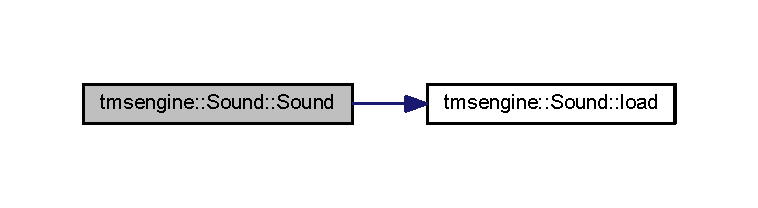
\includegraphics[width=350pt]{classtmsengine_1_1_sound_a666456cd06cec8089d5be3fce56132f1_cgraph}
\end{center}
\end{figure}


\subsection{Member Function Documentation}
\mbox{\Hypertarget{classtmsengine_1_1_sound_aca383fe0b166a15eae25580e1e1e8d41}\label{classtmsengine_1_1_sound_aca383fe0b166a15eae25580e1e1e8d41}} 
\index{tmsengine\+::\+Sound@{tmsengine\+::\+Sound}!load@{load}}
\index{load@{load}!tmsengine\+::\+Sound@{tmsengine\+::\+Sound}}
\subsubsection{\texorpdfstring{load()}{load()}}
{\footnotesize\ttfamily void tmsengine\+::\+Sound\+::load (\begin{DoxyParamCaption}\item[{std\+::string}]{path }\end{DoxyParamCaption})}

Here is the caller graph for this function\+:\nopagebreak
\begin{figure}[H]
\begin{center}
\leavevmode
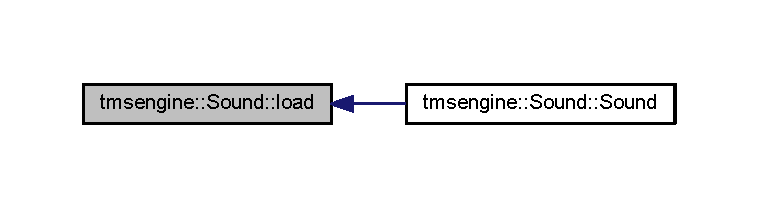
\includegraphics[width=350pt]{classtmsengine_1_1_sound_aca383fe0b166a15eae25580e1e1e8d41_icgraph}
\end{center}
\end{figure}
\mbox{\Hypertarget{classtmsengine_1_1_sound_aeb5717b4ce5f64b7c1e696f471730486}\label{classtmsengine_1_1_sound_aeb5717b4ce5f64b7c1e696f471730486}} 
\index{tmsengine\+::\+Sound@{tmsengine\+::\+Sound}!play@{play}}
\index{play@{play}!tmsengine\+::\+Sound@{tmsengine\+::\+Sound}}
\subsubsection{\texorpdfstring{play()}{play()}\hspace{0.1cm}{\footnotesize\ttfamily [1/2]}}
{\footnotesize\ttfamily void tmsengine\+::\+Sound\+::play (\begin{DoxyParamCaption}\item[{float}]{vol,  }\item[{float}]{min,  }\item[{float}]{max }\end{DoxyParamCaption})}

\mbox{\Hypertarget{classtmsengine_1_1_sound_a842d33a838588ed6a4652b427faa5e0a}\label{classtmsengine_1_1_sound_a842d33a838588ed6a4652b427faa5e0a}} 
\index{tmsengine\+::\+Sound@{tmsengine\+::\+Sound}!play@{play}}
\index{play@{play}!tmsengine\+::\+Sound@{tmsengine\+::\+Sound}}
\subsubsection{\texorpdfstring{play()}{play()}\hspace{0.1cm}{\footnotesize\ttfamily [2/2]}}
{\footnotesize\ttfamily void tmsengine\+::\+Sound\+::play (\begin{DoxyParamCaption}{ }\end{DoxyParamCaption})}



\subsection{Member Data Documentation}
\mbox{\Hypertarget{classtmsengine_1_1_sound_ac6c9ad2ebd7410f0cdc0d58a3891a5b8}\label{classtmsengine_1_1_sound_ac6c9ad2ebd7410f0cdc0d58a3891a5b8}} 
\index{tmsengine\+::\+Sound@{tmsengine\+::\+Sound}!impl@{impl}}
\index{impl@{impl}!tmsengine\+::\+Sound@{tmsengine\+::\+Sound}}
\subsubsection{\texorpdfstring{impl}{impl}}
{\footnotesize\ttfamily std\+::shared\+\_\+ptr$<$\hyperlink{structtmsengine_1_1_sound_impl}{Sound\+Impl}$>$ tmsengine\+::\+Sound\+::impl\hspace{0.3cm}{\ttfamily [private]}}



The documentation for this class was generated from the following files\+:\begin{DoxyCompactItemize}
\item 
T\+M\+S\+Engine/\hyperlink{_sound_8h}{Sound.\+h}\item 
T\+M\+S\+Engine/\hyperlink{_sound_8cpp}{Sound.\+cpp}\end{DoxyCompactItemize}

\hypertarget{structtmsengine_1_1_sound_impl}{}\section{tmsengine\+:\+:Sound\+Impl Struct Reference}
\label{structtmsengine_1_1_sound_impl}\index{tmsengine\+::\+Sound\+Impl@{tmsengine\+::\+Sound\+Impl}}
\subsection*{Public Member Functions}
\begin{DoxyCompactItemize}
\item 
\hyperlink{structtmsengine_1_1_sound_impl_a96a5387f2e92cd9f856874babc825ac7}{$\sim$\+Sound\+Impl} ()
\item 
void \hyperlink{structtmsengine_1_1_sound_impl_a1995d7987e588d66baa614381d0613da}{load\+\_\+ogg} (std\+::string filename, std\+::vector$<$ char $>$ \&buffer, A\+Lenum \&format, A\+Lsizei \&freq)
\end{DoxyCompactItemize}
\subsection*{Public Attributes}
\begin{DoxyCompactItemize}
\item 
A\+Luint \hyperlink{structtmsengine_1_1_sound_impl_a2d9069b4af77273e7bfe07f063486244}{sound\+ID}
\end{DoxyCompactItemize}


\subsection{Constructor \& Destructor Documentation}
\mbox{\Hypertarget{structtmsengine_1_1_sound_impl_a96a5387f2e92cd9f856874babc825ac7}\label{structtmsengine_1_1_sound_impl_a96a5387f2e92cd9f856874babc825ac7}} 
\index{tmsengine\+::\+Sound\+Impl@{tmsengine\+::\+Sound\+Impl}!````~Sound\+Impl@{$\sim$\+Sound\+Impl}}
\index{````~Sound\+Impl@{$\sim$\+Sound\+Impl}!tmsengine\+::\+Sound\+Impl@{tmsengine\+::\+Sound\+Impl}}
\subsubsection{\texorpdfstring{$\sim$\+Sound\+Impl()}{~SoundImpl()}}
{\footnotesize\ttfamily tmsengine\+::\+Sound\+Impl\+::$\sim$\+Sound\+Impl (\begin{DoxyParamCaption}{ }\end{DoxyParamCaption})\hspace{0.3cm}{\ttfamily [inline]}}



\subsection{Member Function Documentation}
\mbox{\Hypertarget{structtmsengine_1_1_sound_impl_a1995d7987e588d66baa614381d0613da}\label{structtmsengine_1_1_sound_impl_a1995d7987e588d66baa614381d0613da}} 
\index{tmsengine\+::\+Sound\+Impl@{tmsengine\+::\+Sound\+Impl}!load\+\_\+ogg@{load\+\_\+ogg}}
\index{load\+\_\+ogg@{load\+\_\+ogg}!tmsengine\+::\+Sound\+Impl@{tmsengine\+::\+Sound\+Impl}}
\subsubsection{\texorpdfstring{load\+\_\+ogg()}{load\_ogg()}}
{\footnotesize\ttfamily void tmsengine\+::\+Sound\+Impl\+::load\+\_\+ogg (\begin{DoxyParamCaption}\item[{std\+::string}]{filename,  }\item[{std\+::vector$<$ char $>$ \&}]{buffer,  }\item[{A\+Lenum \&}]{format,  }\item[{A\+Lsizei \&}]{freq }\end{DoxyParamCaption})\hspace{0.3cm}{\ttfamily [inline]}}



\subsection{Member Data Documentation}
\mbox{\Hypertarget{structtmsengine_1_1_sound_impl_a2d9069b4af77273e7bfe07f063486244}\label{structtmsengine_1_1_sound_impl_a2d9069b4af77273e7bfe07f063486244}} 
\index{tmsengine\+::\+Sound\+Impl@{tmsengine\+::\+Sound\+Impl}!sound\+ID@{sound\+ID}}
\index{sound\+ID@{sound\+ID}!tmsengine\+::\+Sound\+Impl@{tmsengine\+::\+Sound\+Impl}}
\subsubsection{\texorpdfstring{sound\+ID}{soundID}}
{\footnotesize\ttfamily A\+Luint tmsengine\+::\+Sound\+Impl\+::sound\+ID}



The documentation for this struct was generated from the following file\+:\begin{DoxyCompactItemize}
\item 
T\+M\+S\+Engine/\hyperlink{_sound_8cpp}{Sound.\+cpp}\end{DoxyCompactItemize}

\hypertarget{classtmsengine_1_1_texture}{}\section{tmsengine\+:\+:Texture Class Reference}
\label{classtmsengine_1_1_texture}\index{tmsengine\+::\+Texture@{tmsengine\+::\+Texture}}


{\ttfamily \#include $<$Texture.\+h$>$}

\subsection*{Public Member Functions}
\begin{DoxyCompactItemize}
\item 
\hyperlink{classtmsengine_1_1_texture_a73f0e6bf5515ee744e3b04ff1899297f}{Texture} (std\+::string path)
\item 
\hyperlink{classtmsengine_1_1_texture_a3985bc791d34dd2c9f3aad02b8095a97}{$\sim$\+Texture} ()
\item 
G\+Luint \hyperlink{classtmsengine_1_1_texture_ab0328c347b63d7b7291c24aa59f2168c}{get\+ID} ()
\item 
glm\+::vec2 \hyperlink{classtmsengine_1_1_texture_a4a1851f9fca94e2fe5c1cc4d723167d1}{get\+Size} ()
\end{DoxyCompactItemize}
\subsection*{Private Member Functions}
\begin{DoxyCompactItemize}
\item 
std\+::shared\+\_\+ptr$<$ \hyperlink{classtmsengine_1_1_texture}{Texture} $>$ \hyperlink{classtmsengine_1_1_texture_a34e2d3a96afc3f1882f32b7ed93497c0}{create} (unsigned int width, unsigned int height)
\item 
std\+::shared\+\_\+ptr$<$ \hyperlink{classtmsengine_1_1_texture}{Texture} $>$ \hyperlink{classtmsengine_1_1_texture_aebb7c646b34ce4ef328194a8948b1753}{load} (std\+::string path)
\end{DoxyCompactItemize}
\subsection*{Private Attributes}
\begin{DoxyCompactItemize}
\item 
G\+Luint \hyperlink{classtmsengine_1_1_texture_a4dfe526efa0addb02849a4f88a9b299a}{ID}
\item 
bool \hyperlink{classtmsengine_1_1_texture_af638b68fbf939afa705fb1d4b788a98d}{dirty}
\item 
int \hyperlink{classtmsengine_1_1_texture_a611e350120e816da2bfc77fca2a5a7e7}{type}
\item 
glm\+::vec2 \hyperlink{classtmsengine_1_1_texture_a2de0e5f3fe721ae3f7dc6b27ea03d752}{size}
\end{DoxyCompactItemize}


\subsection{Constructor \& Destructor Documentation}
\mbox{\Hypertarget{classtmsengine_1_1_texture_a73f0e6bf5515ee744e3b04ff1899297f}\label{classtmsengine_1_1_texture_a73f0e6bf5515ee744e3b04ff1899297f}} 
\index{tmsengine\+::\+Texture@{tmsengine\+::\+Texture}!Texture@{Texture}}
\index{Texture@{Texture}!tmsengine\+::\+Texture@{tmsengine\+::\+Texture}}
\subsubsection{\texorpdfstring{Texture()}{Texture()}}
{\footnotesize\ttfamily tmsengine\+::\+Texture\+::\+Texture (\begin{DoxyParamCaption}\item[{std\+::string}]{path }\end{DoxyParamCaption})}

\mbox{\Hypertarget{classtmsengine_1_1_texture_a3985bc791d34dd2c9f3aad02b8095a97}\label{classtmsengine_1_1_texture_a3985bc791d34dd2c9f3aad02b8095a97}} 
\index{tmsengine\+::\+Texture@{tmsengine\+::\+Texture}!````~Texture@{$\sim$\+Texture}}
\index{````~Texture@{$\sim$\+Texture}!tmsengine\+::\+Texture@{tmsengine\+::\+Texture}}
\subsubsection{\texorpdfstring{$\sim$\+Texture()}{~Texture()}}
{\footnotesize\ttfamily tmsengine\+::\+Texture\+::$\sim$\+Texture (\begin{DoxyParamCaption}{ }\end{DoxyParamCaption})}



\subsection{Member Function Documentation}
\mbox{\Hypertarget{classtmsengine_1_1_texture_a34e2d3a96afc3f1882f32b7ed93497c0}\label{classtmsengine_1_1_texture_a34e2d3a96afc3f1882f32b7ed93497c0}} 
\index{tmsengine\+::\+Texture@{tmsengine\+::\+Texture}!create@{create}}
\index{create@{create}!tmsengine\+::\+Texture@{tmsengine\+::\+Texture}}
\subsubsection{\texorpdfstring{create()}{create()}}
{\footnotesize\ttfamily std\+::shared\+\_\+ptr$<$\hyperlink{classtmsengine_1_1_texture}{Texture}$>$ tmsengine\+::\+Texture\+::create (\begin{DoxyParamCaption}\item[{unsigned int}]{width,  }\item[{unsigned int}]{height }\end{DoxyParamCaption})\hspace{0.3cm}{\ttfamily [private]}}

\mbox{\Hypertarget{classtmsengine_1_1_texture_ab0328c347b63d7b7291c24aa59f2168c}\label{classtmsengine_1_1_texture_ab0328c347b63d7b7291c24aa59f2168c}} 
\index{tmsengine\+::\+Texture@{tmsengine\+::\+Texture}!get\+ID@{get\+ID}}
\index{get\+ID@{get\+ID}!tmsengine\+::\+Texture@{tmsengine\+::\+Texture}}
\subsubsection{\texorpdfstring{get\+I\+D()}{getID()}}
{\footnotesize\ttfamily G\+Luint tmsengine\+::\+Texture\+::get\+ID (\begin{DoxyParamCaption}{ }\end{DoxyParamCaption})}

\mbox{\Hypertarget{classtmsengine_1_1_texture_a4a1851f9fca94e2fe5c1cc4d723167d1}\label{classtmsengine_1_1_texture_a4a1851f9fca94e2fe5c1cc4d723167d1}} 
\index{tmsengine\+::\+Texture@{tmsengine\+::\+Texture}!get\+Size@{get\+Size}}
\index{get\+Size@{get\+Size}!tmsengine\+::\+Texture@{tmsengine\+::\+Texture}}
\subsubsection{\texorpdfstring{get\+Size()}{getSize()}}
{\footnotesize\ttfamily glm\+::vec2 tmsengine\+::\+Texture\+::get\+Size (\begin{DoxyParamCaption}{ }\end{DoxyParamCaption})}

\mbox{\Hypertarget{classtmsengine_1_1_texture_aebb7c646b34ce4ef328194a8948b1753}\label{classtmsengine_1_1_texture_aebb7c646b34ce4ef328194a8948b1753}} 
\index{tmsengine\+::\+Texture@{tmsengine\+::\+Texture}!load@{load}}
\index{load@{load}!tmsengine\+::\+Texture@{tmsengine\+::\+Texture}}
\subsubsection{\texorpdfstring{load()}{load()}}
{\footnotesize\ttfamily std\+::shared\+\_\+ptr$<$\hyperlink{classtmsengine_1_1_texture}{Texture}$>$ tmsengine\+::\+Texture\+::load (\begin{DoxyParamCaption}\item[{std\+::string}]{path }\end{DoxyParamCaption})\hspace{0.3cm}{\ttfamily [private]}}



\subsection{Member Data Documentation}
\mbox{\Hypertarget{classtmsengine_1_1_texture_af638b68fbf939afa705fb1d4b788a98d}\label{classtmsengine_1_1_texture_af638b68fbf939afa705fb1d4b788a98d}} 
\index{tmsengine\+::\+Texture@{tmsengine\+::\+Texture}!dirty@{dirty}}
\index{dirty@{dirty}!tmsengine\+::\+Texture@{tmsengine\+::\+Texture}}
\subsubsection{\texorpdfstring{dirty}{dirty}}
{\footnotesize\ttfamily bool tmsengine\+::\+Texture\+::dirty\hspace{0.3cm}{\ttfamily [private]}}

\mbox{\Hypertarget{classtmsengine_1_1_texture_a4dfe526efa0addb02849a4f88a9b299a}\label{classtmsengine_1_1_texture_a4dfe526efa0addb02849a4f88a9b299a}} 
\index{tmsengine\+::\+Texture@{tmsengine\+::\+Texture}!ID@{ID}}
\index{ID@{ID}!tmsengine\+::\+Texture@{tmsengine\+::\+Texture}}
\subsubsection{\texorpdfstring{ID}{ID}}
{\footnotesize\ttfamily G\+Luint tmsengine\+::\+Texture\+::\+ID\hspace{0.3cm}{\ttfamily [private]}}

\mbox{\Hypertarget{classtmsengine_1_1_texture_a2de0e5f3fe721ae3f7dc6b27ea03d752}\label{classtmsengine_1_1_texture_a2de0e5f3fe721ae3f7dc6b27ea03d752}} 
\index{tmsengine\+::\+Texture@{tmsengine\+::\+Texture}!size@{size}}
\index{size@{size}!tmsengine\+::\+Texture@{tmsengine\+::\+Texture}}
\subsubsection{\texorpdfstring{size}{size}}
{\footnotesize\ttfamily glm\+::vec2 tmsengine\+::\+Texture\+::size\hspace{0.3cm}{\ttfamily [private]}}

\mbox{\Hypertarget{classtmsengine_1_1_texture_a611e350120e816da2bfc77fca2a5a7e7}\label{classtmsengine_1_1_texture_a611e350120e816da2bfc77fca2a5a7e7}} 
\index{tmsengine\+::\+Texture@{tmsengine\+::\+Texture}!type@{type}}
\index{type@{type}!tmsengine\+::\+Texture@{tmsengine\+::\+Texture}}
\subsubsection{\texorpdfstring{type}{type}}
{\footnotesize\ttfamily int tmsengine\+::\+Texture\+::type\hspace{0.3cm}{\ttfamily [private]}}



The documentation for this class was generated from the following files\+:\begin{DoxyCompactItemize}
\item 
T\+M\+S\+Engine/\+Resources/\hyperlink{_texture_8h}{Texture.\+h}\item 
T\+M\+S\+Engine/\+Resources/\hyperlink{_texture_8cpp}{Texture.\+cpp}\end{DoxyCompactItemize}

\hypertarget{classtmsengine_1_1_transform}{}\section{tmsengine\+:\+:Transform Class Reference}
\label{classtmsengine_1_1_transform}\index{tmsengine\+::\+Transform@{tmsengine\+::\+Transform}}


{\ttfamily \#include $<$Transform.\+h$>$}



Inheritance diagram for tmsengine\+:\+:Transform\+:\nopagebreak
\begin{figure}[H]
\begin{center}
\leavevmode
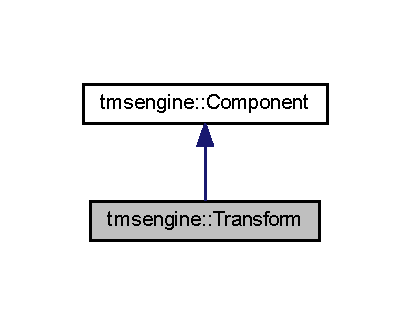
\includegraphics[width=197pt]{classtmsengine_1_1_transform__inherit__graph}
\end{center}
\end{figure}


Collaboration diagram for tmsengine\+:\+:Transform\+:\nopagebreak
\begin{figure}[H]
\begin{center}
\leavevmode
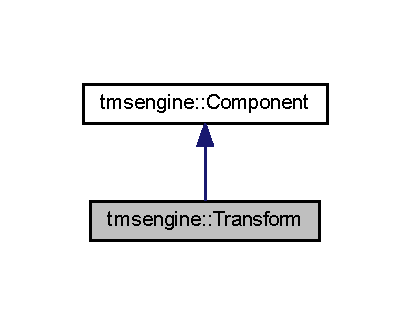
\includegraphics[width=197pt]{classtmsengine_1_1_transform__coll__graph}
\end{center}
\end{figure}
\subsection*{Public Member Functions}
\begin{DoxyCompactItemize}
\item 
void \hyperlink{classtmsengine_1_1_transform_a761046214917103b7286e36cde981c00}{on\+Init} ()
\item 
void \hyperlink{classtmsengine_1_1_transform_a9b5c3f77a33d065a7c35c3f125f411c9}{translate} (glm\+::vec3 amount)
\item 
void \hyperlink{classtmsengine_1_1_transform_a4252393f36c4dac7665366dc6d046b2c}{rotate} (glm\+::vec3 amount)
\item 
void \hyperlink{classtmsengine_1_1_transform_abb597d75f70663d2eb39de63d8d55fb7}{Scale} (glm\+::vec3 amount)
\item 
void \hyperlink{classtmsengine_1_1_transform_a3dee28280ad81f1e45b1b85a1a6fe400}{set\+Position} (glm\+::vec3 \hyperlink{classtmsengine_1_1_transform_a588c0d056219dbe15a97c727a36880aa}{position})
\item 
void \hyperlink{classtmsengine_1_1_transform_a64a3902ef95913ce9cdcc586060e8478}{set\+Rotation} (glm\+::vec3 \hyperlink{classtmsengine_1_1_transform_a3dfc7b3c7d5cebed1168fd124a81803c}{rotation})
\item 
void \hyperlink{classtmsengine_1_1_transform_ae70b645863286dd4ef06b2ff3dc93db9}{set\+Scale} (glm\+::vec3 \+\_\+scale)
\item 
glm\+::vec3 \hyperlink{classtmsengine_1_1_transform_a44891a7afedd2d98670f4031e44d62c4}{get\+Position} ()
\item 
glm\+::vec3 \hyperlink{classtmsengine_1_1_transform_a0a1fcbfe44cf518b01a3b2806e4fd305}{get\+Rotation} ()
\item 
glm\+::vec3 \hyperlink{classtmsengine_1_1_transform_aa42e86916a3979d625d60beb91f982c6}{get\+Scale} ()
\end{DoxyCompactItemize}
\subsection*{Private Attributes}
\begin{DoxyCompactItemize}
\item 
glm\+::vec3 \hyperlink{classtmsengine_1_1_transform_a588c0d056219dbe15a97c727a36880aa}{position}
\item 
glm\+::vec3 \hyperlink{classtmsengine_1_1_transform_a3dfc7b3c7d5cebed1168fd124a81803c}{rotation}
\item 
glm\+::vec3 \hyperlink{classtmsengine_1_1_transform_a7a166d9bb060a56975ffb75dba91ee58}{scale}
\end{DoxyCompactItemize}


\subsection{Member Function Documentation}
\mbox{\Hypertarget{classtmsengine_1_1_transform_a44891a7afedd2d98670f4031e44d62c4}\label{classtmsengine_1_1_transform_a44891a7afedd2d98670f4031e44d62c4}} 
\index{tmsengine\+::\+Transform@{tmsengine\+::\+Transform}!get\+Position@{get\+Position}}
\index{get\+Position@{get\+Position}!tmsengine\+::\+Transform@{tmsengine\+::\+Transform}}
\subsubsection{\texorpdfstring{get\+Position()}{getPosition()}}
{\footnotesize\ttfamily glm\+::vec3 tmsengine\+::\+Transform\+::get\+Position (\begin{DoxyParamCaption}{ }\end{DoxyParamCaption})}

\mbox{\Hypertarget{classtmsengine_1_1_transform_a0a1fcbfe44cf518b01a3b2806e4fd305}\label{classtmsengine_1_1_transform_a0a1fcbfe44cf518b01a3b2806e4fd305}} 
\index{tmsengine\+::\+Transform@{tmsengine\+::\+Transform}!get\+Rotation@{get\+Rotation}}
\index{get\+Rotation@{get\+Rotation}!tmsengine\+::\+Transform@{tmsengine\+::\+Transform}}
\subsubsection{\texorpdfstring{get\+Rotation()}{getRotation()}}
{\footnotesize\ttfamily glm\+::vec3 tmsengine\+::\+Transform\+::get\+Rotation (\begin{DoxyParamCaption}{ }\end{DoxyParamCaption})}

\mbox{\Hypertarget{classtmsengine_1_1_transform_aa42e86916a3979d625d60beb91f982c6}\label{classtmsengine_1_1_transform_aa42e86916a3979d625d60beb91f982c6}} 
\index{tmsengine\+::\+Transform@{tmsengine\+::\+Transform}!get\+Scale@{get\+Scale}}
\index{get\+Scale@{get\+Scale}!tmsengine\+::\+Transform@{tmsengine\+::\+Transform}}
\subsubsection{\texorpdfstring{get\+Scale()}{getScale()}}
{\footnotesize\ttfamily glm\+::vec3 tmsengine\+::\+Transform\+::get\+Scale (\begin{DoxyParamCaption}{ }\end{DoxyParamCaption})}

\mbox{\Hypertarget{classtmsengine_1_1_transform_a761046214917103b7286e36cde981c00}\label{classtmsengine_1_1_transform_a761046214917103b7286e36cde981c00}} 
\index{tmsengine\+::\+Transform@{tmsengine\+::\+Transform}!on\+Init@{on\+Init}}
\index{on\+Init@{on\+Init}!tmsengine\+::\+Transform@{tmsengine\+::\+Transform}}
\subsubsection{\texorpdfstring{on\+Init()}{onInit()}}
{\footnotesize\ttfamily void tmsengine\+::\+Transform\+::on\+Init (\begin{DoxyParamCaption}{ }\end{DoxyParamCaption})\hspace{0.3cm}{\ttfamily [virtual]}}



Reimplemented from \hyperlink{classtmsengine_1_1_component_ae992e9b0c98b569eba13d0274089bc18}{tmsengine\+::\+Component}.

Here is the call graph for this function\+:\nopagebreak
\begin{figure}[H]
\begin{center}
\leavevmode
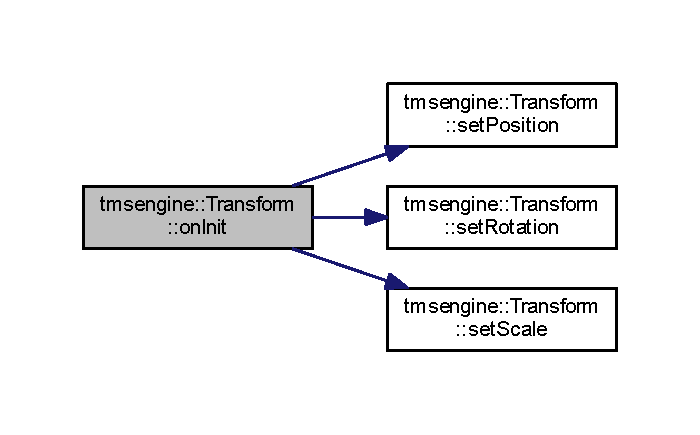
\includegraphics[width=336pt]{classtmsengine_1_1_transform_a761046214917103b7286e36cde981c00_cgraph}
\end{center}
\end{figure}
\mbox{\Hypertarget{classtmsengine_1_1_transform_a4252393f36c4dac7665366dc6d046b2c}\label{classtmsengine_1_1_transform_a4252393f36c4dac7665366dc6d046b2c}} 
\index{tmsengine\+::\+Transform@{tmsengine\+::\+Transform}!rotate@{rotate}}
\index{rotate@{rotate}!tmsengine\+::\+Transform@{tmsengine\+::\+Transform}}
\subsubsection{\texorpdfstring{rotate()}{rotate()}}
{\footnotesize\ttfamily void tmsengine\+::\+Transform\+::rotate (\begin{DoxyParamCaption}\item[{glm\+::vec3}]{amount }\end{DoxyParamCaption})}

\mbox{\Hypertarget{classtmsengine_1_1_transform_abb597d75f70663d2eb39de63d8d55fb7}\label{classtmsengine_1_1_transform_abb597d75f70663d2eb39de63d8d55fb7}} 
\index{tmsengine\+::\+Transform@{tmsengine\+::\+Transform}!Scale@{Scale}}
\index{Scale@{Scale}!tmsengine\+::\+Transform@{tmsengine\+::\+Transform}}
\subsubsection{\texorpdfstring{Scale()}{Scale()}}
{\footnotesize\ttfamily void tmsengine\+::\+Transform\+::\+Scale (\begin{DoxyParamCaption}\item[{glm\+::vec3}]{amount }\end{DoxyParamCaption})}

\mbox{\Hypertarget{classtmsengine_1_1_transform_a3dee28280ad81f1e45b1b85a1a6fe400}\label{classtmsengine_1_1_transform_a3dee28280ad81f1e45b1b85a1a6fe400}} 
\index{tmsengine\+::\+Transform@{tmsengine\+::\+Transform}!set\+Position@{set\+Position}}
\index{set\+Position@{set\+Position}!tmsengine\+::\+Transform@{tmsengine\+::\+Transform}}
\subsubsection{\texorpdfstring{set\+Position()}{setPosition()}}
{\footnotesize\ttfamily void tmsengine\+::\+Transform\+::set\+Position (\begin{DoxyParamCaption}\item[{glm\+::vec3}]{position }\end{DoxyParamCaption})}

Here is the caller graph for this function\+:\nopagebreak
\begin{figure}[H]
\begin{center}
\leavevmode
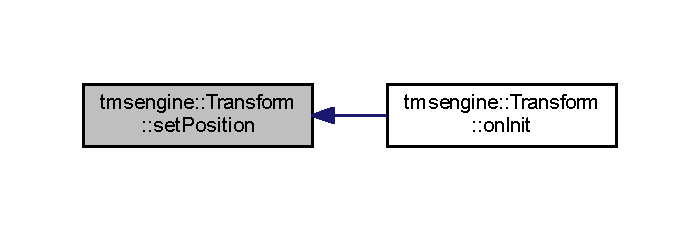
\includegraphics[width=336pt]{classtmsengine_1_1_transform_a3dee28280ad81f1e45b1b85a1a6fe400_icgraph}
\end{center}
\end{figure}
\mbox{\Hypertarget{classtmsengine_1_1_transform_a64a3902ef95913ce9cdcc586060e8478}\label{classtmsengine_1_1_transform_a64a3902ef95913ce9cdcc586060e8478}} 
\index{tmsengine\+::\+Transform@{tmsengine\+::\+Transform}!set\+Rotation@{set\+Rotation}}
\index{set\+Rotation@{set\+Rotation}!tmsengine\+::\+Transform@{tmsengine\+::\+Transform}}
\subsubsection{\texorpdfstring{set\+Rotation()}{setRotation()}}
{\footnotesize\ttfamily void tmsengine\+::\+Transform\+::set\+Rotation (\begin{DoxyParamCaption}\item[{glm\+::vec3}]{rotation }\end{DoxyParamCaption})}

Here is the caller graph for this function\+:\nopagebreak
\begin{figure}[H]
\begin{center}
\leavevmode
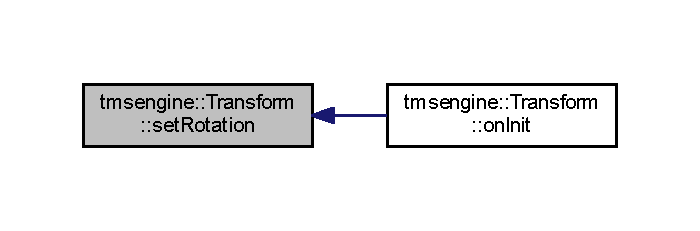
\includegraphics[width=336pt]{classtmsengine_1_1_transform_a64a3902ef95913ce9cdcc586060e8478_icgraph}
\end{center}
\end{figure}
\mbox{\Hypertarget{classtmsengine_1_1_transform_ae70b645863286dd4ef06b2ff3dc93db9}\label{classtmsengine_1_1_transform_ae70b645863286dd4ef06b2ff3dc93db9}} 
\index{tmsengine\+::\+Transform@{tmsengine\+::\+Transform}!set\+Scale@{set\+Scale}}
\index{set\+Scale@{set\+Scale}!tmsengine\+::\+Transform@{tmsengine\+::\+Transform}}
\subsubsection{\texorpdfstring{set\+Scale()}{setScale()}}
{\footnotesize\ttfamily void tmsengine\+::\+Transform\+::set\+Scale (\begin{DoxyParamCaption}\item[{glm\+::vec3}]{\+\_\+scale }\end{DoxyParamCaption})}

Here is the caller graph for this function\+:\nopagebreak
\begin{figure}[H]
\begin{center}
\leavevmode
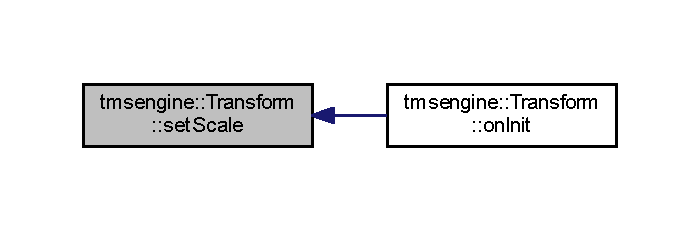
\includegraphics[width=336pt]{classtmsengine_1_1_transform_ae70b645863286dd4ef06b2ff3dc93db9_icgraph}
\end{center}
\end{figure}
\mbox{\Hypertarget{classtmsengine_1_1_transform_a9b5c3f77a33d065a7c35c3f125f411c9}\label{classtmsengine_1_1_transform_a9b5c3f77a33d065a7c35c3f125f411c9}} 
\index{tmsengine\+::\+Transform@{tmsengine\+::\+Transform}!translate@{translate}}
\index{translate@{translate}!tmsengine\+::\+Transform@{tmsengine\+::\+Transform}}
\subsubsection{\texorpdfstring{translate()}{translate()}}
{\footnotesize\ttfamily void tmsengine\+::\+Transform\+::translate (\begin{DoxyParamCaption}\item[{glm\+::vec3}]{amount }\end{DoxyParamCaption})}



\subsection{Member Data Documentation}
\mbox{\Hypertarget{classtmsengine_1_1_transform_a588c0d056219dbe15a97c727a36880aa}\label{classtmsengine_1_1_transform_a588c0d056219dbe15a97c727a36880aa}} 
\index{tmsengine\+::\+Transform@{tmsengine\+::\+Transform}!position@{position}}
\index{position@{position}!tmsengine\+::\+Transform@{tmsengine\+::\+Transform}}
\subsubsection{\texorpdfstring{position}{position}}
{\footnotesize\ttfamily glm\+::vec3 tmsengine\+::\+Transform\+::position\hspace{0.3cm}{\ttfamily [private]}}

\mbox{\Hypertarget{classtmsengine_1_1_transform_a3dfc7b3c7d5cebed1168fd124a81803c}\label{classtmsengine_1_1_transform_a3dfc7b3c7d5cebed1168fd124a81803c}} 
\index{tmsengine\+::\+Transform@{tmsengine\+::\+Transform}!rotation@{rotation}}
\index{rotation@{rotation}!tmsengine\+::\+Transform@{tmsengine\+::\+Transform}}
\subsubsection{\texorpdfstring{rotation}{rotation}}
{\footnotesize\ttfamily glm\+::vec3 tmsengine\+::\+Transform\+::rotation\hspace{0.3cm}{\ttfamily [private]}}

\mbox{\Hypertarget{classtmsengine_1_1_transform_a7a166d9bb060a56975ffb75dba91ee58}\label{classtmsengine_1_1_transform_a7a166d9bb060a56975ffb75dba91ee58}} 
\index{tmsengine\+::\+Transform@{tmsengine\+::\+Transform}!scale@{scale}}
\index{scale@{scale}!tmsengine\+::\+Transform@{tmsengine\+::\+Transform}}
\subsubsection{\texorpdfstring{scale}{scale}}
{\footnotesize\ttfamily glm\+::vec3 tmsengine\+::\+Transform\+::scale\hspace{0.3cm}{\ttfamily [private]}}



The documentation for this class was generated from the following files\+:\begin{DoxyCompactItemize}
\item 
T\+M\+S\+Engine/\hyperlink{_transform_8h}{Transform.\+h}\item 
T\+M\+S\+Engine/\hyperlink{_transform_8cpp}{Transform.\+cpp}\end{DoxyCompactItemize}

\hypertarget{struct_triangle}{}\section{Triangle Struct Reference}
\label{struct_triangle}\index{Triangle@{Triangle}}


{\ttfamily \#include $<$Mesh.\+h$>$}

\subsection*{Public Attributes}
\begin{DoxyCompactItemize}
\item 
glm\+::vec3 \hyperlink{struct_triangle_a75a142a237477a294d9625379a6076d7}{a}
\item 
glm\+::vec3 \hyperlink{struct_triangle_a926bd99a7e345b5527ccbee07f0e6b0b}{b}
\item 
glm\+::vec3 \hyperlink{struct_triangle_aaad6c6cb9cf100dd36798fc3e34b1936}{c}
\end{DoxyCompactItemize}


\subsection{Member Data Documentation}
\mbox{\Hypertarget{struct_triangle_a75a142a237477a294d9625379a6076d7}\label{struct_triangle_a75a142a237477a294d9625379a6076d7}} 
\index{Triangle@{Triangle}!a@{a}}
\index{a@{a}!Triangle@{Triangle}}
\subsubsection{\texorpdfstring{a}{a}}
{\footnotesize\ttfamily glm\+::vec3 Triangle\+::a}

\mbox{\Hypertarget{struct_triangle_a926bd99a7e345b5527ccbee07f0e6b0b}\label{struct_triangle_a926bd99a7e345b5527ccbee07f0e6b0b}} 
\index{Triangle@{Triangle}!b@{b}}
\index{b@{b}!Triangle@{Triangle}}
\subsubsection{\texorpdfstring{b}{b}}
{\footnotesize\ttfamily glm\+::vec3 Triangle\+::b}

\mbox{\Hypertarget{struct_triangle_aaad6c6cb9cf100dd36798fc3e34b1936}\label{struct_triangle_aaad6c6cb9cf100dd36798fc3e34b1936}} 
\index{Triangle@{Triangle}!c@{c}}
\index{c@{c}!Triangle@{Triangle}}
\subsubsection{\texorpdfstring{c}{c}}
{\footnotesize\ttfamily glm\+::vec3 Triangle\+::c}



The documentation for this struct was generated from the following file\+:\begin{DoxyCompactItemize}
\item 
T\+M\+S\+Engine/\+Resources/\hyperlink{_mesh_8h}{Mesh.\+h}\end{DoxyCompactItemize}

\hypertarget{classtmsengine_1_1_vertex_array}{}\section{tmsengine\+:\+:Vertex\+Array Class Reference}
\label{classtmsengine_1_1_vertex_array}\index{tmsengine\+::\+Vertex\+Array@{tmsengine\+::\+Vertex\+Array}}


{\ttfamily \#include $<$Vertex\+Array.\+h$>$}

\subsection*{Public Member Functions}
\begin{DoxyCompactItemize}
\item 
\hyperlink{classtmsengine_1_1_vertex_array_ab8a2dcce9698f96dac5f9a19c6979d03}{Vertex\+Array} ()
\item 
\hyperlink{classtmsengine_1_1_vertex_array_ad3790c015fab2f4ca0ac32b1782b7f33}{Vertex\+Array} (std\+::string path)
\item 
void \hyperlink{classtmsengine_1_1_vertex_array_aded817cf210e13abd10b92475718e3ef}{set\+Buffer} (std\+::string attribute, std\+::shared\+\_\+ptr$<$ \hyperlink{classtmsengine_1_1_vertex_buffer}{Vertex\+Buffer} $>$ buffer)
\item 
int \hyperlink{classtmsengine_1_1_vertex_array_abd774aebfb2cac21e6b5b769b24839ab}{get\+Vertex\+Count} ()
\item 
G\+Luint \hyperlink{classtmsengine_1_1_vertex_array_ab8d9e0c4130f9a0880be869c5f176285}{get\+ID} ()
\end{DoxyCompactItemize}
\subsection*{Private Member Functions}
\begin{DoxyCompactItemize}
\item 
void \hyperlink{classtmsengine_1_1_vertex_array_a35f3a952fe7089d2ebe71c6d4e2c2443}{split\+String\+White\+Space} (std\+::string \&input, std\+::vector$<$ std\+::string $>$ \&output)
\item 
void \hyperlink{classtmsengine_1_1_vertex_array_a0d589e02258c90f551011be850f180e4}{split\+String} (std\+::string \&input, char splitter, std\+::vector$<$ std\+::string $>$ \&output)
\end{DoxyCompactItemize}
\subsection*{Private Attributes}
\begin{DoxyCompactItemize}
\item 
G\+Luint \hyperlink{classtmsengine_1_1_vertex_array_a4a18394cce9fe71f003ab23721fba532}{vao\+ID}
\item 
std\+::vector$<$ std\+::shared\+\_\+ptr$<$ \hyperlink{classtmsengine_1_1_vertex_buffer}{Vertex\+Buffer} $>$ $>$ \hyperlink{classtmsengine_1_1_vertex_array_a39afaa4b9e37f5a8e107e82cab67e354}{buffers}
\item 
bool \hyperlink{classtmsengine_1_1_vertex_array_a9d53a5e75ce6c4afec5091ebeb17069f}{dirty}
\end{DoxyCompactItemize}


\subsection{Constructor \& Destructor Documentation}
\mbox{\Hypertarget{classtmsengine_1_1_vertex_array_ab8a2dcce9698f96dac5f9a19c6979d03}\label{classtmsengine_1_1_vertex_array_ab8a2dcce9698f96dac5f9a19c6979d03}} 
\index{tmsengine\+::\+Vertex\+Array@{tmsengine\+::\+Vertex\+Array}!Vertex\+Array@{Vertex\+Array}}
\index{Vertex\+Array@{Vertex\+Array}!tmsengine\+::\+Vertex\+Array@{tmsengine\+::\+Vertex\+Array}}
\subsubsection{\texorpdfstring{Vertex\+Array()}{VertexArray()}\hspace{0.1cm}{\footnotesize\ttfamily [1/2]}}
{\footnotesize\ttfamily Vertex\+Array\+::\+Vertex\+Array (\begin{DoxyParamCaption}{ }\end{DoxyParamCaption})}

\mbox{\Hypertarget{classtmsengine_1_1_vertex_array_ad3790c015fab2f4ca0ac32b1782b7f33}\label{classtmsengine_1_1_vertex_array_ad3790c015fab2f4ca0ac32b1782b7f33}} 
\index{tmsengine\+::\+Vertex\+Array@{tmsengine\+::\+Vertex\+Array}!Vertex\+Array@{Vertex\+Array}}
\index{Vertex\+Array@{Vertex\+Array}!tmsengine\+::\+Vertex\+Array@{tmsengine\+::\+Vertex\+Array}}
\subsubsection{\texorpdfstring{Vertex\+Array()}{VertexArray()}\hspace{0.1cm}{\footnotesize\ttfamily [2/2]}}
{\footnotesize\ttfamily Vertex\+Array\+::\+Vertex\+Array (\begin{DoxyParamCaption}\item[{std\+::string}]{path }\end{DoxyParamCaption})}

Here is the call graph for this function\+:\nopagebreak
\begin{figure}[H]
\begin{center}
\leavevmode
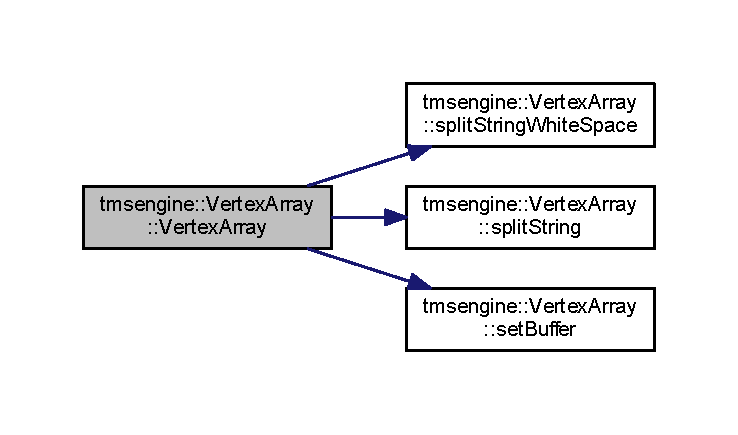
\includegraphics[width=350pt]{classtmsengine_1_1_vertex_array_ad3790c015fab2f4ca0ac32b1782b7f33_cgraph}
\end{center}
\end{figure}


\subsection{Member Function Documentation}
\mbox{\Hypertarget{classtmsengine_1_1_vertex_array_ab8d9e0c4130f9a0880be869c5f176285}\label{classtmsengine_1_1_vertex_array_ab8d9e0c4130f9a0880be869c5f176285}} 
\index{tmsengine\+::\+Vertex\+Array@{tmsengine\+::\+Vertex\+Array}!get\+ID@{get\+ID}}
\index{get\+ID@{get\+ID}!tmsengine\+::\+Vertex\+Array@{tmsengine\+::\+Vertex\+Array}}
\subsubsection{\texorpdfstring{get\+I\+D()}{getID()}}
{\footnotesize\ttfamily G\+Luint Vertex\+Array\+::get\+ID (\begin{DoxyParamCaption}{ }\end{DoxyParamCaption})}

\mbox{\Hypertarget{classtmsengine_1_1_vertex_array_abd774aebfb2cac21e6b5b769b24839ab}\label{classtmsengine_1_1_vertex_array_abd774aebfb2cac21e6b5b769b24839ab}} 
\index{tmsengine\+::\+Vertex\+Array@{tmsengine\+::\+Vertex\+Array}!get\+Vertex\+Count@{get\+Vertex\+Count}}
\index{get\+Vertex\+Count@{get\+Vertex\+Count}!tmsengine\+::\+Vertex\+Array@{tmsengine\+::\+Vertex\+Array}}
\subsubsection{\texorpdfstring{get\+Vertex\+Count()}{getVertexCount()}}
{\footnotesize\ttfamily int Vertex\+Array\+::get\+Vertex\+Count (\begin{DoxyParamCaption}{ }\end{DoxyParamCaption})}

\mbox{\Hypertarget{classtmsengine_1_1_vertex_array_aded817cf210e13abd10b92475718e3ef}\label{classtmsengine_1_1_vertex_array_aded817cf210e13abd10b92475718e3ef}} 
\index{tmsengine\+::\+Vertex\+Array@{tmsengine\+::\+Vertex\+Array}!set\+Buffer@{set\+Buffer}}
\index{set\+Buffer@{set\+Buffer}!tmsengine\+::\+Vertex\+Array@{tmsengine\+::\+Vertex\+Array}}
\subsubsection{\texorpdfstring{set\+Buffer()}{setBuffer()}}
{\footnotesize\ttfamily void Vertex\+Array\+::set\+Buffer (\begin{DoxyParamCaption}\item[{std\+::string}]{attribute,  }\item[{std\+::shared\+\_\+ptr$<$ \hyperlink{classtmsengine_1_1_vertex_buffer}{Vertex\+Buffer} $>$}]{buffer }\end{DoxyParamCaption})}

Here is the caller graph for this function\+:\nopagebreak
\begin{figure}[H]
\begin{center}
\leavevmode
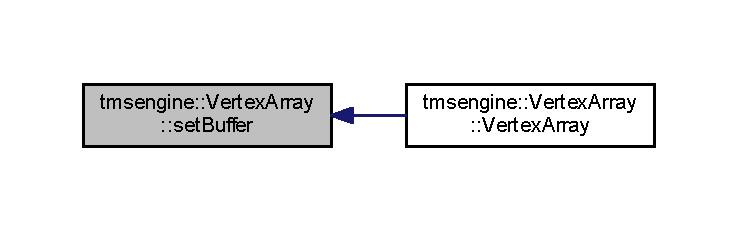
\includegraphics[width=350pt]{classtmsengine_1_1_vertex_array_aded817cf210e13abd10b92475718e3ef_icgraph}
\end{center}
\end{figure}
\mbox{\Hypertarget{classtmsengine_1_1_vertex_array_a0d589e02258c90f551011be850f180e4}\label{classtmsengine_1_1_vertex_array_a0d589e02258c90f551011be850f180e4}} 
\index{tmsengine\+::\+Vertex\+Array@{tmsengine\+::\+Vertex\+Array}!split\+String@{split\+String}}
\index{split\+String@{split\+String}!tmsengine\+::\+Vertex\+Array@{tmsengine\+::\+Vertex\+Array}}
\subsubsection{\texorpdfstring{split\+String()}{splitString()}}
{\footnotesize\ttfamily void Vertex\+Array\+::split\+String (\begin{DoxyParamCaption}\item[{std\+::string \&}]{input,  }\item[{char}]{splitter,  }\item[{std\+::vector$<$ std\+::string $>$ \&}]{output }\end{DoxyParamCaption})\hspace{0.3cm}{\ttfamily [private]}}

Here is the caller graph for this function\+:\nopagebreak
\begin{figure}[H]
\begin{center}
\leavevmode
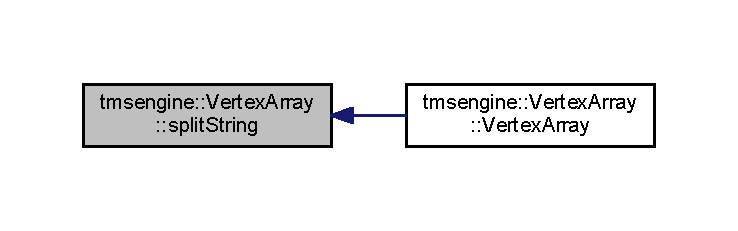
\includegraphics[width=350pt]{classtmsengine_1_1_vertex_array_a0d589e02258c90f551011be850f180e4_icgraph}
\end{center}
\end{figure}
\mbox{\Hypertarget{classtmsengine_1_1_vertex_array_a35f3a952fe7089d2ebe71c6d4e2c2443}\label{classtmsengine_1_1_vertex_array_a35f3a952fe7089d2ebe71c6d4e2c2443}} 
\index{tmsengine\+::\+Vertex\+Array@{tmsengine\+::\+Vertex\+Array}!split\+String\+White\+Space@{split\+String\+White\+Space}}
\index{split\+String\+White\+Space@{split\+String\+White\+Space}!tmsengine\+::\+Vertex\+Array@{tmsengine\+::\+Vertex\+Array}}
\subsubsection{\texorpdfstring{split\+String\+White\+Space()}{splitStringWhiteSpace()}}
{\footnotesize\ttfamily void Vertex\+Array\+::split\+String\+White\+Space (\begin{DoxyParamCaption}\item[{std\+::string \&}]{input,  }\item[{std\+::vector$<$ std\+::string $>$ \&}]{output }\end{DoxyParamCaption})\hspace{0.3cm}{\ttfamily [private]}}

Here is the caller graph for this function\+:\nopagebreak
\begin{figure}[H]
\begin{center}
\leavevmode
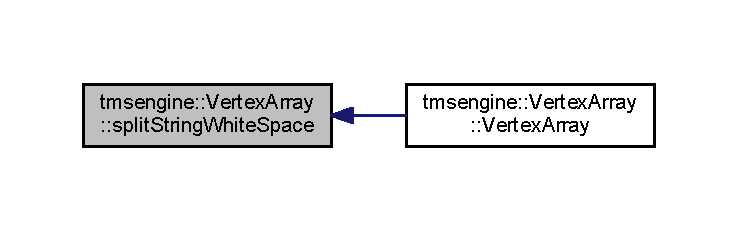
\includegraphics[width=350pt]{classtmsengine_1_1_vertex_array_a35f3a952fe7089d2ebe71c6d4e2c2443_icgraph}
\end{center}
\end{figure}


\subsection{Member Data Documentation}
\mbox{\Hypertarget{classtmsengine_1_1_vertex_array_a39afaa4b9e37f5a8e107e82cab67e354}\label{classtmsengine_1_1_vertex_array_a39afaa4b9e37f5a8e107e82cab67e354}} 
\index{tmsengine\+::\+Vertex\+Array@{tmsengine\+::\+Vertex\+Array}!buffers@{buffers}}
\index{buffers@{buffers}!tmsengine\+::\+Vertex\+Array@{tmsengine\+::\+Vertex\+Array}}
\subsubsection{\texorpdfstring{buffers}{buffers}}
{\footnotesize\ttfamily std\+::vector$<$std\+::shared\+\_\+ptr$<$\hyperlink{classtmsengine_1_1_vertex_buffer}{Vertex\+Buffer}$>$ $>$ tmsengine\+::\+Vertex\+Array\+::buffers\hspace{0.3cm}{\ttfamily [private]}}

\mbox{\Hypertarget{classtmsengine_1_1_vertex_array_a9d53a5e75ce6c4afec5091ebeb17069f}\label{classtmsengine_1_1_vertex_array_a9d53a5e75ce6c4afec5091ebeb17069f}} 
\index{tmsengine\+::\+Vertex\+Array@{tmsengine\+::\+Vertex\+Array}!dirty@{dirty}}
\index{dirty@{dirty}!tmsengine\+::\+Vertex\+Array@{tmsengine\+::\+Vertex\+Array}}
\subsubsection{\texorpdfstring{dirty}{dirty}}
{\footnotesize\ttfamily bool tmsengine\+::\+Vertex\+Array\+::dirty\hspace{0.3cm}{\ttfamily [private]}}

\mbox{\Hypertarget{classtmsengine_1_1_vertex_array_a4a18394cce9fe71f003ab23721fba532}\label{classtmsengine_1_1_vertex_array_a4a18394cce9fe71f003ab23721fba532}} 
\index{tmsengine\+::\+Vertex\+Array@{tmsengine\+::\+Vertex\+Array}!vao\+ID@{vao\+ID}}
\index{vao\+ID@{vao\+ID}!tmsengine\+::\+Vertex\+Array@{tmsengine\+::\+Vertex\+Array}}
\subsubsection{\texorpdfstring{vao\+ID}{vaoID}}
{\footnotesize\ttfamily G\+Luint tmsengine\+::\+Vertex\+Array\+::vao\+ID\hspace{0.3cm}{\ttfamily [private]}}



The documentation for this class was generated from the following files\+:\begin{DoxyCompactItemize}
\item 
T\+M\+S\+Engine/\hyperlink{_vertex_array_8h}{Vertex\+Array.\+h}\item 
T\+M\+S\+Engine/\hyperlink{_vertex_array_8cpp}{Vertex\+Array.\+cpp}\end{DoxyCompactItemize}

\hypertarget{classtmsengine_1_1_vertex_buffer}{}\section{tmsengine\+:\+:Vertex\+Buffer Class Reference}
\label{classtmsengine_1_1_vertex_buffer}\index{tmsengine\+::\+Vertex\+Buffer@{tmsengine\+::\+Vertex\+Buffer}}


{\ttfamily \#include $<$Vertex\+Buffer.\+h$>$}

\subsection*{Public Member Functions}
\begin{DoxyCompactItemize}
\item 
\hyperlink{classtmsengine_1_1_vertex_buffer_adb25d82a47ad82d5b69a75ac111401b8}{Vertex\+Buffer} ()
\item 
void \hyperlink{classtmsengine_1_1_vertex_buffer_ab1bf2eaca95ef9eaf2bacfa19dfbde5a}{add} (glm\+::vec2 value)
\item 
void \hyperlink{classtmsengine_1_1_vertex_buffer_a9c6d5ca7265694557c2f9142070eedc6}{add} (glm\+::vec3 value)
\item 
void \hyperlink{classtmsengine_1_1_vertex_buffer_adbaf46d318f9d12447e557f2a226fb03}{add} (glm\+::vec4 value)
\item 
int \hyperlink{classtmsengine_1_1_vertex_buffer_a765c3bda21961cd07f3422fd4cb4c2b5}{get\+Components} ()
\item 
int \hyperlink{classtmsengine_1_1_vertex_buffer_a1af72090f8fea7f93f43de8cefba9f4e}{get\+Data\+Size} ()
\item 
G\+Luint \hyperlink{classtmsengine_1_1_vertex_buffer_a5183f22e3747065c2ac77d50fa3935f4}{get\+ID} ()
\end{DoxyCompactItemize}
\subsection*{Private Attributes}
\begin{DoxyCompactItemize}
\item 
G\+Luint \hyperlink{classtmsengine_1_1_vertex_buffer_ab42f1676b7f61ab1b0e3ad9167914c41}{vbo\+ID}
\item 
int \hyperlink{classtmsengine_1_1_vertex_buffer_a1e06450b89acd7b5b73c85e2187908ca}{components}
\item 
bool \hyperlink{classtmsengine_1_1_vertex_buffer_a6b9ac4bfeff0c6dfe9a964246fef2824}{dirty}
\item 
std\+::vector$<$ G\+Lfloat $>$ \hyperlink{classtmsengine_1_1_vertex_buffer_aaf04b009201c9d710044c0bc748017e0}{data}
\end{DoxyCompactItemize}


\subsection{Constructor \& Destructor Documentation}
\mbox{\Hypertarget{classtmsengine_1_1_vertex_buffer_adb25d82a47ad82d5b69a75ac111401b8}\label{classtmsengine_1_1_vertex_buffer_adb25d82a47ad82d5b69a75ac111401b8}} 
\index{tmsengine\+::\+Vertex\+Buffer@{tmsengine\+::\+Vertex\+Buffer}!Vertex\+Buffer@{Vertex\+Buffer}}
\index{Vertex\+Buffer@{Vertex\+Buffer}!tmsengine\+::\+Vertex\+Buffer@{tmsengine\+::\+Vertex\+Buffer}}
\subsubsection{\texorpdfstring{Vertex\+Buffer()}{VertexBuffer()}}
{\footnotesize\ttfamily Vertex\+Buffer\+::\+Vertex\+Buffer (\begin{DoxyParamCaption}{ }\end{DoxyParamCaption})}



\subsection{Member Function Documentation}
\mbox{\Hypertarget{classtmsengine_1_1_vertex_buffer_ab1bf2eaca95ef9eaf2bacfa19dfbde5a}\label{classtmsengine_1_1_vertex_buffer_ab1bf2eaca95ef9eaf2bacfa19dfbde5a}} 
\index{tmsengine\+::\+Vertex\+Buffer@{tmsengine\+::\+Vertex\+Buffer}!add@{add}}
\index{add@{add}!tmsengine\+::\+Vertex\+Buffer@{tmsengine\+::\+Vertex\+Buffer}}
\subsubsection{\texorpdfstring{add()}{add()}\hspace{0.1cm}{\footnotesize\ttfamily [1/3]}}
{\footnotesize\ttfamily void Vertex\+Buffer\+::add (\begin{DoxyParamCaption}\item[{glm\+::vec2}]{value }\end{DoxyParamCaption})}

\mbox{\Hypertarget{classtmsengine_1_1_vertex_buffer_a9c6d5ca7265694557c2f9142070eedc6}\label{classtmsengine_1_1_vertex_buffer_a9c6d5ca7265694557c2f9142070eedc6}} 
\index{tmsengine\+::\+Vertex\+Buffer@{tmsengine\+::\+Vertex\+Buffer}!add@{add}}
\index{add@{add}!tmsengine\+::\+Vertex\+Buffer@{tmsengine\+::\+Vertex\+Buffer}}
\subsubsection{\texorpdfstring{add()}{add()}\hspace{0.1cm}{\footnotesize\ttfamily [2/3]}}
{\footnotesize\ttfamily void Vertex\+Buffer\+::add (\begin{DoxyParamCaption}\item[{glm\+::vec3}]{value }\end{DoxyParamCaption})}

\mbox{\Hypertarget{classtmsengine_1_1_vertex_buffer_adbaf46d318f9d12447e557f2a226fb03}\label{classtmsengine_1_1_vertex_buffer_adbaf46d318f9d12447e557f2a226fb03}} 
\index{tmsengine\+::\+Vertex\+Buffer@{tmsengine\+::\+Vertex\+Buffer}!add@{add}}
\index{add@{add}!tmsengine\+::\+Vertex\+Buffer@{tmsengine\+::\+Vertex\+Buffer}}
\subsubsection{\texorpdfstring{add()}{add()}\hspace{0.1cm}{\footnotesize\ttfamily [3/3]}}
{\footnotesize\ttfamily void Vertex\+Buffer\+::add (\begin{DoxyParamCaption}\item[{glm\+::vec4}]{value }\end{DoxyParamCaption})}

\mbox{\Hypertarget{classtmsengine_1_1_vertex_buffer_a765c3bda21961cd07f3422fd4cb4c2b5}\label{classtmsengine_1_1_vertex_buffer_a765c3bda21961cd07f3422fd4cb4c2b5}} 
\index{tmsengine\+::\+Vertex\+Buffer@{tmsengine\+::\+Vertex\+Buffer}!get\+Components@{get\+Components}}
\index{get\+Components@{get\+Components}!tmsengine\+::\+Vertex\+Buffer@{tmsengine\+::\+Vertex\+Buffer}}
\subsubsection{\texorpdfstring{get\+Components()}{getComponents()}}
{\footnotesize\ttfamily int Vertex\+Buffer\+::get\+Components (\begin{DoxyParamCaption}{ }\end{DoxyParamCaption})}

\mbox{\Hypertarget{classtmsengine_1_1_vertex_buffer_a1af72090f8fea7f93f43de8cefba9f4e}\label{classtmsengine_1_1_vertex_buffer_a1af72090f8fea7f93f43de8cefba9f4e}} 
\index{tmsengine\+::\+Vertex\+Buffer@{tmsengine\+::\+Vertex\+Buffer}!get\+Data\+Size@{get\+Data\+Size}}
\index{get\+Data\+Size@{get\+Data\+Size}!tmsengine\+::\+Vertex\+Buffer@{tmsengine\+::\+Vertex\+Buffer}}
\subsubsection{\texorpdfstring{get\+Data\+Size()}{getDataSize()}}
{\footnotesize\ttfamily int Vertex\+Buffer\+::get\+Data\+Size (\begin{DoxyParamCaption}{ }\end{DoxyParamCaption})}

\mbox{\Hypertarget{classtmsengine_1_1_vertex_buffer_a5183f22e3747065c2ac77d50fa3935f4}\label{classtmsengine_1_1_vertex_buffer_a5183f22e3747065c2ac77d50fa3935f4}} 
\index{tmsengine\+::\+Vertex\+Buffer@{tmsengine\+::\+Vertex\+Buffer}!get\+ID@{get\+ID}}
\index{get\+ID@{get\+ID}!tmsengine\+::\+Vertex\+Buffer@{tmsengine\+::\+Vertex\+Buffer}}
\subsubsection{\texorpdfstring{get\+I\+D()}{getID()}}
{\footnotesize\ttfamily G\+Luint Vertex\+Buffer\+::get\+ID (\begin{DoxyParamCaption}{ }\end{DoxyParamCaption})}



\subsection{Member Data Documentation}
\mbox{\Hypertarget{classtmsengine_1_1_vertex_buffer_a1e06450b89acd7b5b73c85e2187908ca}\label{classtmsengine_1_1_vertex_buffer_a1e06450b89acd7b5b73c85e2187908ca}} 
\index{tmsengine\+::\+Vertex\+Buffer@{tmsengine\+::\+Vertex\+Buffer}!components@{components}}
\index{components@{components}!tmsengine\+::\+Vertex\+Buffer@{tmsengine\+::\+Vertex\+Buffer}}
\subsubsection{\texorpdfstring{components}{components}}
{\footnotesize\ttfamily int tmsengine\+::\+Vertex\+Buffer\+::components\hspace{0.3cm}{\ttfamily [private]}}

\mbox{\Hypertarget{classtmsengine_1_1_vertex_buffer_aaf04b009201c9d710044c0bc748017e0}\label{classtmsengine_1_1_vertex_buffer_aaf04b009201c9d710044c0bc748017e0}} 
\index{tmsengine\+::\+Vertex\+Buffer@{tmsengine\+::\+Vertex\+Buffer}!data@{data}}
\index{data@{data}!tmsengine\+::\+Vertex\+Buffer@{tmsengine\+::\+Vertex\+Buffer}}
\subsubsection{\texorpdfstring{data}{data}}
{\footnotesize\ttfamily std\+::vector$<$G\+Lfloat$>$ tmsengine\+::\+Vertex\+Buffer\+::data\hspace{0.3cm}{\ttfamily [private]}}

\mbox{\Hypertarget{classtmsengine_1_1_vertex_buffer_a6b9ac4bfeff0c6dfe9a964246fef2824}\label{classtmsengine_1_1_vertex_buffer_a6b9ac4bfeff0c6dfe9a964246fef2824}} 
\index{tmsengine\+::\+Vertex\+Buffer@{tmsengine\+::\+Vertex\+Buffer}!dirty@{dirty}}
\index{dirty@{dirty}!tmsengine\+::\+Vertex\+Buffer@{tmsengine\+::\+Vertex\+Buffer}}
\subsubsection{\texorpdfstring{dirty}{dirty}}
{\footnotesize\ttfamily bool tmsengine\+::\+Vertex\+Buffer\+::dirty\hspace{0.3cm}{\ttfamily [private]}}

\mbox{\Hypertarget{classtmsengine_1_1_vertex_buffer_ab42f1676b7f61ab1b0e3ad9167914c41}\label{classtmsengine_1_1_vertex_buffer_ab42f1676b7f61ab1b0e3ad9167914c41}} 
\index{tmsengine\+::\+Vertex\+Buffer@{tmsengine\+::\+Vertex\+Buffer}!vbo\+ID@{vbo\+ID}}
\index{vbo\+ID@{vbo\+ID}!tmsengine\+::\+Vertex\+Buffer@{tmsengine\+::\+Vertex\+Buffer}}
\subsubsection{\texorpdfstring{vbo\+ID}{vboID}}
{\footnotesize\ttfamily G\+Luint tmsengine\+::\+Vertex\+Buffer\+::vbo\+ID\hspace{0.3cm}{\ttfamily [private]}}



The documentation for this class was generated from the following files\+:\begin{DoxyCompactItemize}
\item 
T\+M\+S\+Engine/\hyperlink{_vertex_buffer_8h}{Vertex\+Buffer.\+h}\item 
T\+M\+S\+Engine/\hyperlink{_vertex_buffer_8cpp}{Vertex\+Buffer.\+cpp}\end{DoxyCompactItemize}

\chapter{File Documentation}
\hypertarget{_camera_8cpp}{}\section{T\+M\+S\+Engine/\+Camera.cpp File Reference}
\label{_camera_8cpp}\index{T\+M\+S\+Engine/\+Camera.\+cpp@{T\+M\+S\+Engine/\+Camera.\+cpp}}
{\ttfamily \#include \char`\"{}Camera.\+h\char`\"{}}\newline
Include dependency graph for Camera.\+cpp\+:\nopagebreak
\begin{figure}[H]
\begin{center}
\leavevmode
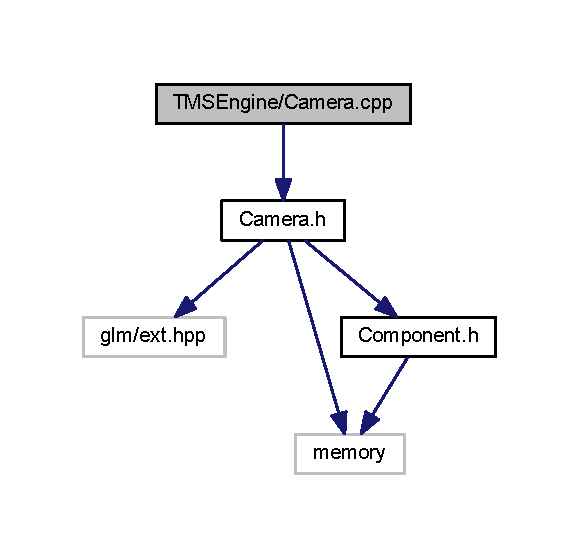
\includegraphics[width=278pt]{_camera_8cpp__incl}
\end{center}
\end{figure}

\hypertarget{_camera_8h}{}\section{T\+M\+S\+Engine/\+Camera.h File Reference}
\label{_camera_8h}\index{T\+M\+S\+Engine/\+Camera.\+h@{T\+M\+S\+Engine/\+Camera.\+h}}
{\ttfamily \#include $<$glm/ext.\+hpp$>$}\newline
{\ttfamily \#include $<$memory$>$}\newline
{\ttfamily \#include \char`\"{}Component.\+h\char`\"{}}\newline
Include dependency graph for Camera.\+h\+:\nopagebreak
\begin{figure}[H]
\begin{center}
\leavevmode
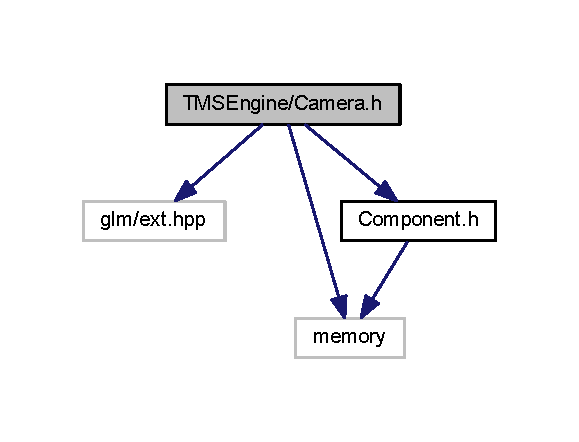
\includegraphics[width=278pt]{_camera_8h__incl}
\end{center}
\end{figure}
This graph shows which files directly or indirectly include this file\+:
\nopagebreak
\begin{figure}[H]
\begin{center}
\leavevmode
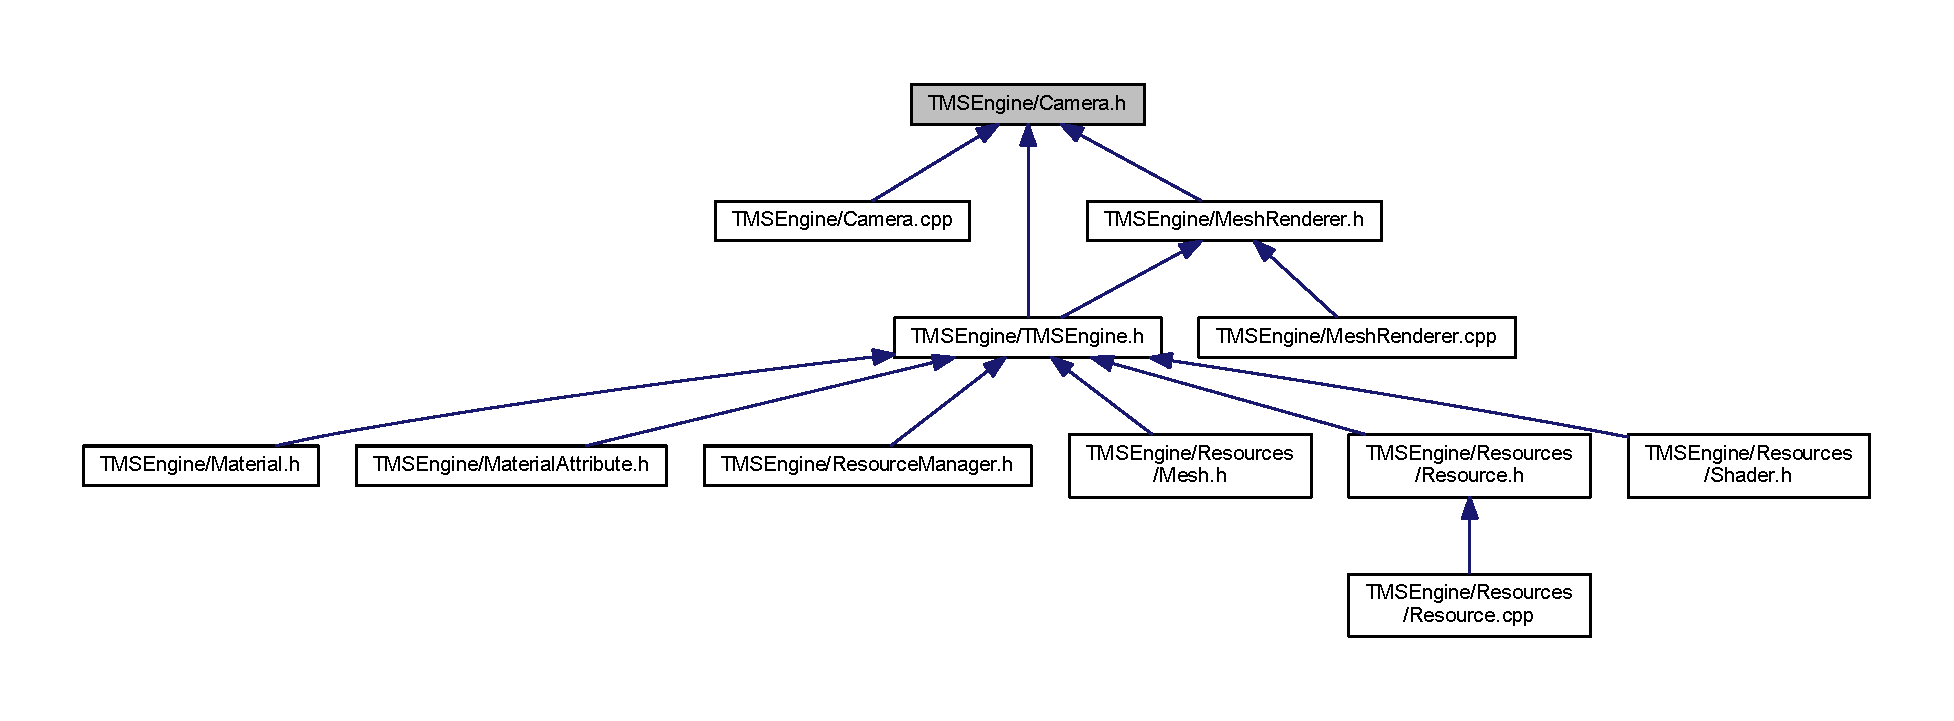
\includegraphics[width=350pt]{_camera_8h__dep__incl}
\end{center}
\end{figure}
\subsection*{Classes}
\begin{DoxyCompactItemize}
\item 
class \hyperlink{classtmsengine_1_1_camera}{tmsengine\+::\+Camera}
\end{DoxyCompactItemize}
\subsection*{Namespaces}
\begin{DoxyCompactItemize}
\item 
 \hyperlink{namespacetmsengine}{tmsengine}
\end{DoxyCompactItemize}

\hypertarget{_component_8cpp}{}\section{T\+M\+S\+Engine/\+Component.cpp File Reference}
\label{_component_8cpp}\index{T\+M\+S\+Engine/\+Component.\+cpp@{T\+M\+S\+Engine/\+Component.\+cpp}}
{\ttfamily \#include \char`\"{}Component.\+h\char`\"{}}\newline
{\ttfamily \#include \char`\"{}Game\+Object.\+h\char`\"{}}\newline
Include dependency graph for Component.\+cpp\+:\nopagebreak
\begin{figure}[H]
\begin{center}
\leavevmode
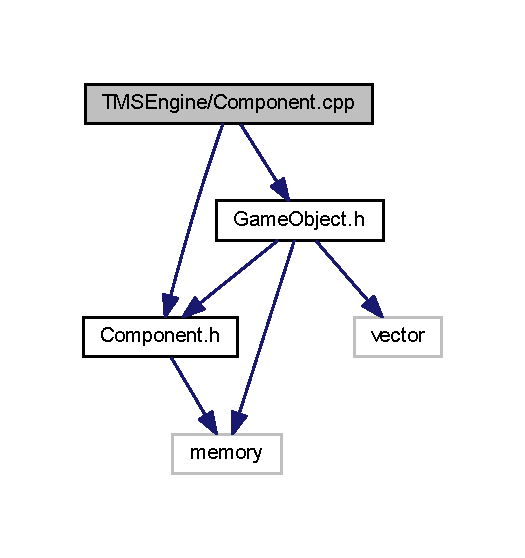
\includegraphics[width=252pt]{_component_8cpp__incl}
\end{center}
\end{figure}
\subsection*{Namespaces}
\begin{DoxyCompactItemize}
\item 
 \hyperlink{namespacetmsengine}{tmsengine}
\end{DoxyCompactItemize}

\hypertarget{_component_8h}{}\section{T\+M\+S\+Engine/\+Component.h File Reference}
\label{_component_8h}\index{T\+M\+S\+Engine/\+Component.\+h@{T\+M\+S\+Engine/\+Component.\+h}}
{\ttfamily \#include $<$memory$>$}\newline
Include dependency graph for Component.\+h\+:\nopagebreak
\begin{figure}[H]
\begin{center}
\leavevmode
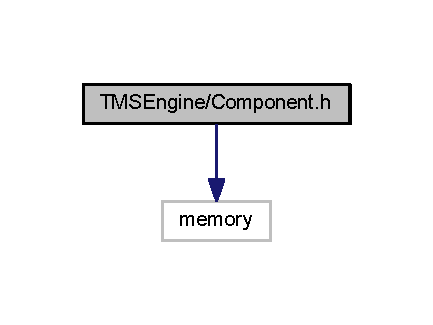
\includegraphics[width=208pt]{_component_8h__incl}
\end{center}
\end{figure}
This graph shows which files directly or indirectly include this file\+:
\nopagebreak
\begin{figure}[H]
\begin{center}
\leavevmode
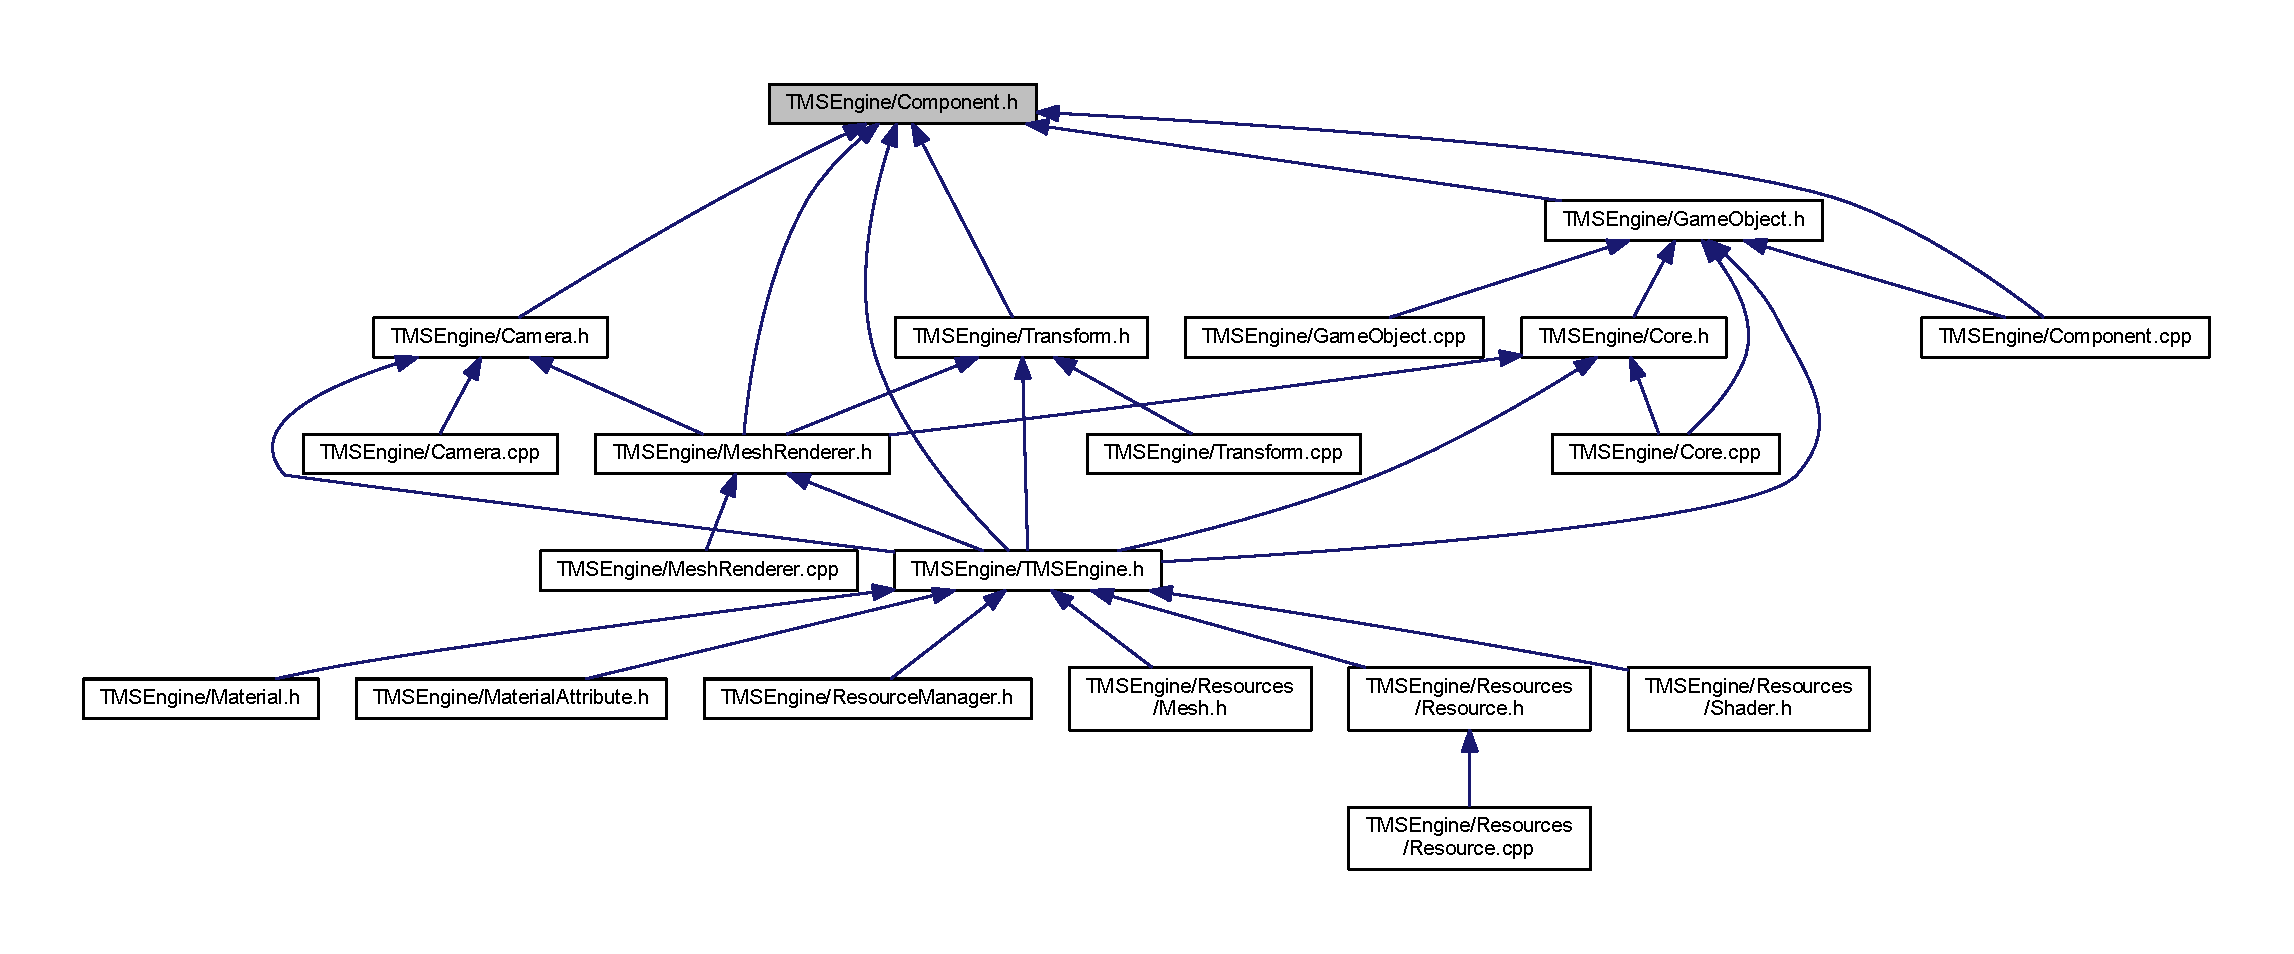
\includegraphics[width=350pt]{_component_8h__dep__incl}
\end{center}
\end{figure}
\subsection*{Classes}
\begin{DoxyCompactItemize}
\item 
class \hyperlink{classtmsengine_1_1_component}{tmsengine\+::\+Component}
\end{DoxyCompactItemize}
\subsection*{Namespaces}
\begin{DoxyCompactItemize}
\item 
 \hyperlink{namespacetmsengine}{tmsengine}
\end{DoxyCompactItemize}
\subsection*{Macros}
\begin{DoxyCompactItemize}
\item 
\#define \hyperlink{_component_8h_a2b7775ab7dd726920f93cb245b14edc5}{T\+M\+S\+E\+N\+G\+I\+N\+E\+\_\+\+C\+O\+M\+P\+O\+N\+E\+N\+T\+\_\+\+H\+\_\+}
\end{DoxyCompactItemize}


\subsection{Macro Definition Documentation}
\mbox{\Hypertarget{_component_8h_a2b7775ab7dd726920f93cb245b14edc5}\label{_component_8h_a2b7775ab7dd726920f93cb245b14edc5}} 
\index{Component.\+h@{Component.\+h}!T\+M\+S\+E\+N\+G\+I\+N\+E\+\_\+\+C\+O\+M\+P\+O\+N\+E\+N\+T\+\_\+\+H\+\_\+@{T\+M\+S\+E\+N\+G\+I\+N\+E\+\_\+\+C\+O\+M\+P\+O\+N\+E\+N\+T\+\_\+\+H\+\_\+}}
\index{T\+M\+S\+E\+N\+G\+I\+N\+E\+\_\+\+C\+O\+M\+P\+O\+N\+E\+N\+T\+\_\+\+H\+\_\+@{T\+M\+S\+E\+N\+G\+I\+N\+E\+\_\+\+C\+O\+M\+P\+O\+N\+E\+N\+T\+\_\+\+H\+\_\+}!Component.\+h@{Component.\+h}}
\subsubsection{\texorpdfstring{T\+M\+S\+E\+N\+G\+I\+N\+E\+\_\+\+C\+O\+M\+P\+O\+N\+E\+N\+T\+\_\+\+H\+\_\+}{TMSENGINE\_COMPONENT\_H\_}}
{\footnotesize\ttfamily \#define T\+M\+S\+E\+N\+G\+I\+N\+E\+\_\+\+C\+O\+M\+P\+O\+N\+E\+N\+T\+\_\+\+H\+\_\+}


\hypertarget{_core_8cpp}{}\section{T\+M\+S\+Engine/\+Core.cpp File Reference}
\label{_core_8cpp}\index{T\+M\+S\+Engine/\+Core.\+cpp@{T\+M\+S\+Engine/\+Core.\+cpp}}
{\ttfamily \#include \char`\"{}Core.\+h\char`\"{}}\newline
{\ttfamily \#include \char`\"{}Game\+Object.\+h\char`\"{}}\newline
{\ttfamily \#include $<$G\+L/glew.\+h$>$}\newline
{\ttfamily \#include $<$glm/ext.\+hpp$>$}\newline
{\ttfamily \#include $<$iostream$>$}\newline
Include dependency graph for Core.\+cpp\+:\nopagebreak
\begin{figure}[H]
\begin{center}
\leavevmode
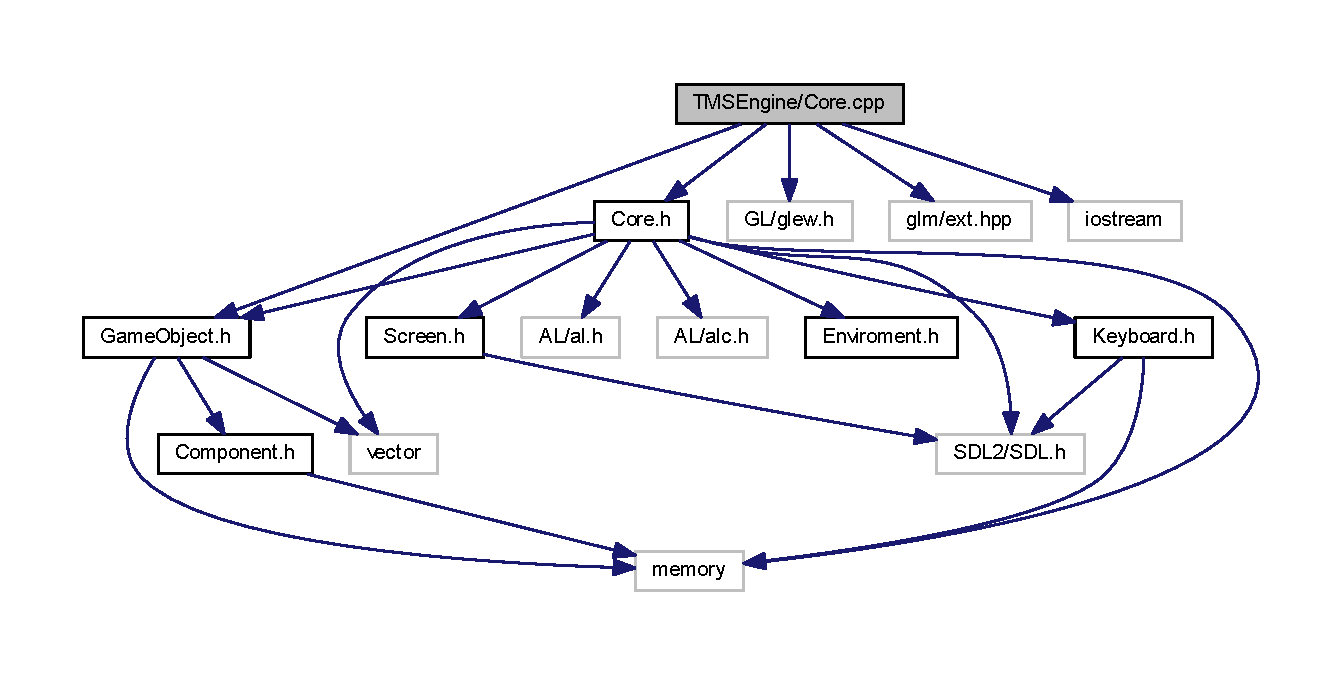
\includegraphics[width=350pt]{_core_8cpp__incl}
\end{center}
\end{figure}
\subsection*{Namespaces}
\begin{DoxyCompactItemize}
\item 
 \hyperlink{namespacetmsengine}{tmsengine}
\end{DoxyCompactItemize}

\hypertarget{_core_8h}{}\section{T\+M\+S\+Engine/\+Core.h File Reference}
\label{_core_8h}\index{T\+M\+S\+Engine/\+Core.\+h@{T\+M\+S\+Engine/\+Core.\+h}}
{\ttfamily \#include $<$S\+D\+L2/\+S\+D\+L.\+h$>$}\newline
{\ttfamily \#include $<$memory$>$}\newline
{\ttfamily \#include $<$vector$>$}\newline
{\ttfamily \#include $<$A\+L/al.\+h$>$}\newline
{\ttfamily \#include $<$A\+L/alc.\+h$>$}\newline
{\ttfamily \#include \char`\"{}Game\+Object.\+h\char`\"{}}\newline
{\ttfamily \#include \char`\"{}Keyboard.\+h\char`\"{}}\newline
{\ttfamily \#include \char`\"{}Enviroment.\+h\char`\"{}}\newline
{\ttfamily \#include \char`\"{}Screen.\+h\char`\"{}}\newline
Include dependency graph for Core.\+h\+:\nopagebreak
\begin{figure}[H]
\begin{center}
\leavevmode
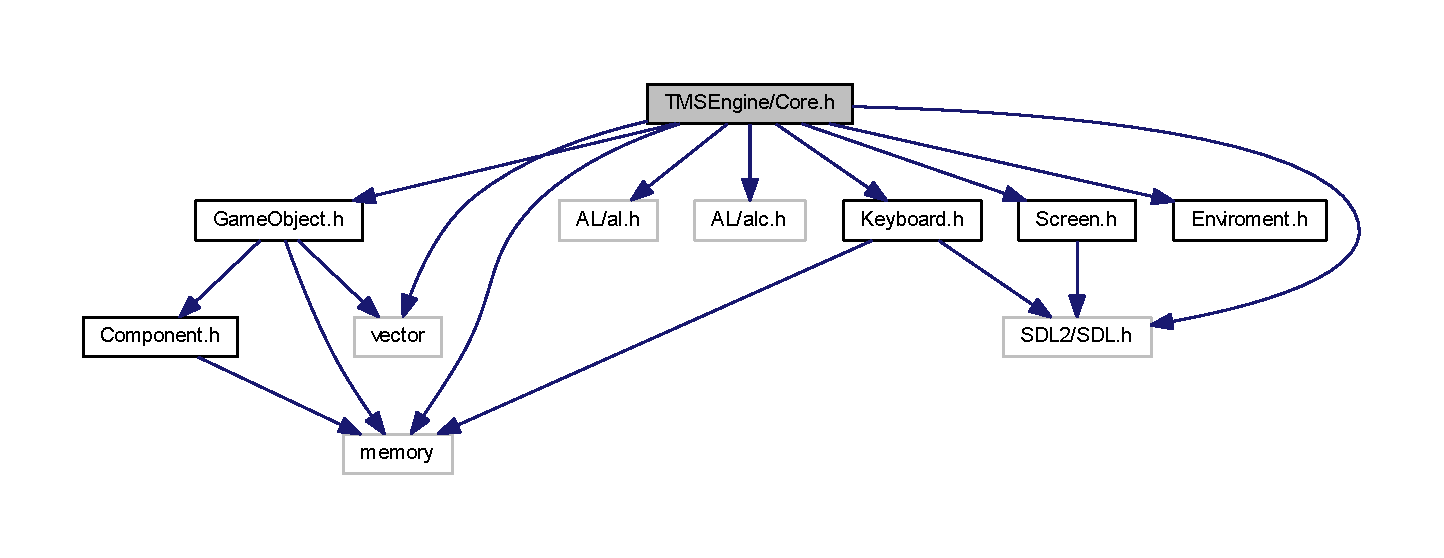
\includegraphics[width=350pt]{_core_8h__incl}
\end{center}
\end{figure}
This graph shows which files directly or indirectly include this file\+:
\nopagebreak
\begin{figure}[H]
\begin{center}
\leavevmode
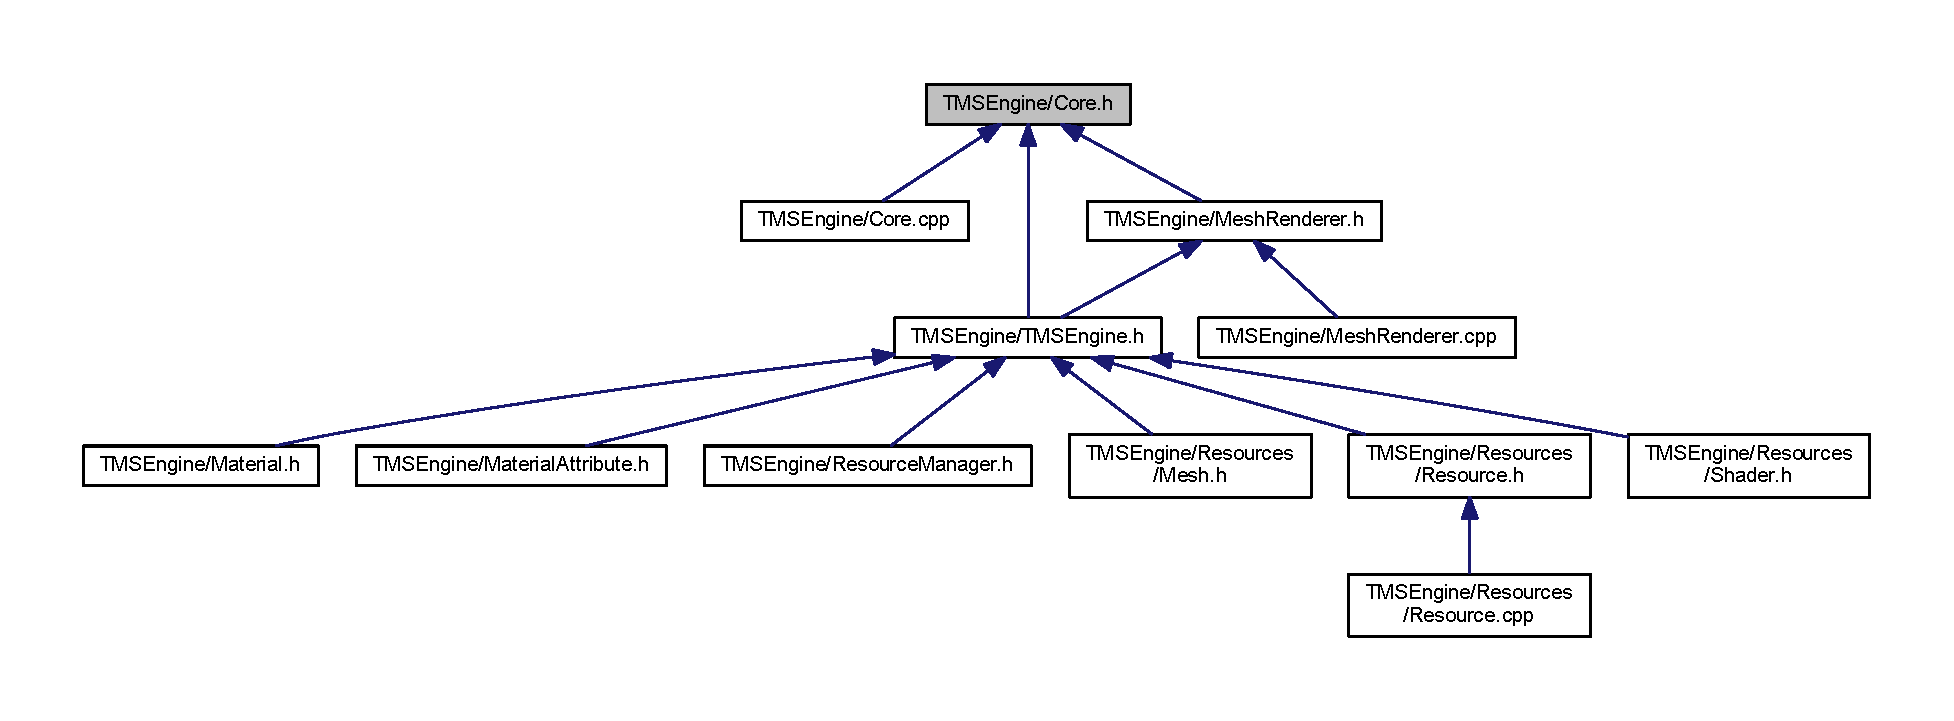
\includegraphics[width=350pt]{_core_8h__dep__incl}
\end{center}
\end{figure}
\subsection*{Classes}
\begin{DoxyCompactItemize}
\item 
class \hyperlink{classtmsengine_1_1_core}{tmsengine\+::\+Core}
\end{DoxyCompactItemize}
\subsection*{Namespaces}
\begin{DoxyCompactItemize}
\item 
 \hyperlink{namespacetmsengine}{tmsengine}
\end{DoxyCompactItemize}

\hypertarget{_enviroment_8cpp}{}\section{T\+M\+S\+Engine/\+Enviroment.cpp File Reference}
\label{_enviroment_8cpp}\index{T\+M\+S\+Engine/\+Enviroment.\+cpp@{T\+M\+S\+Engine/\+Enviroment.\+cpp}}
{\ttfamily \#include \char`\"{}Enviroment.\+h\char`\"{}}\newline
{\ttfamily \#include $<$iostream$>$}\newline
{\ttfamily \#include $<$S\+D\+L2/\+S\+D\+L.\+h$>$}\newline
Include dependency graph for Enviroment.\+cpp\+:\nopagebreak
\begin{figure}[H]
\begin{center}
\leavevmode
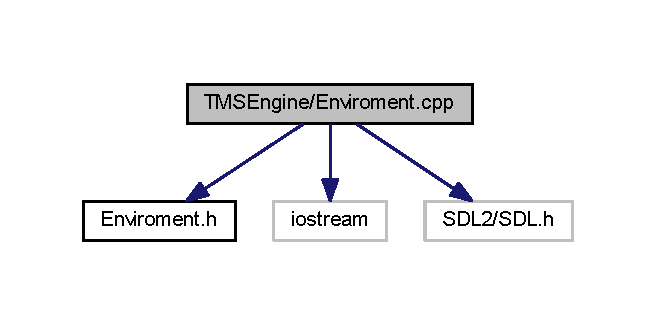
\includegraphics[width=315pt]{_enviroment_8cpp__incl}
\end{center}
\end{figure}
\subsection*{Namespaces}
\begin{DoxyCompactItemize}
\item 
 \hyperlink{namespacetmsengine}{tmsengine}
\end{DoxyCompactItemize}

\hypertarget{_enviroment_8h}{}\section{T\+M\+S\+Engine/\+Enviroment.h File Reference}
\label{_enviroment_8h}\index{T\+M\+S\+Engine/\+Enviroment.\+h@{T\+M\+S\+Engine/\+Enviroment.\+h}}
This graph shows which files directly or indirectly include this file\+:
\nopagebreak
\begin{figure}[H]
\begin{center}
\leavevmode
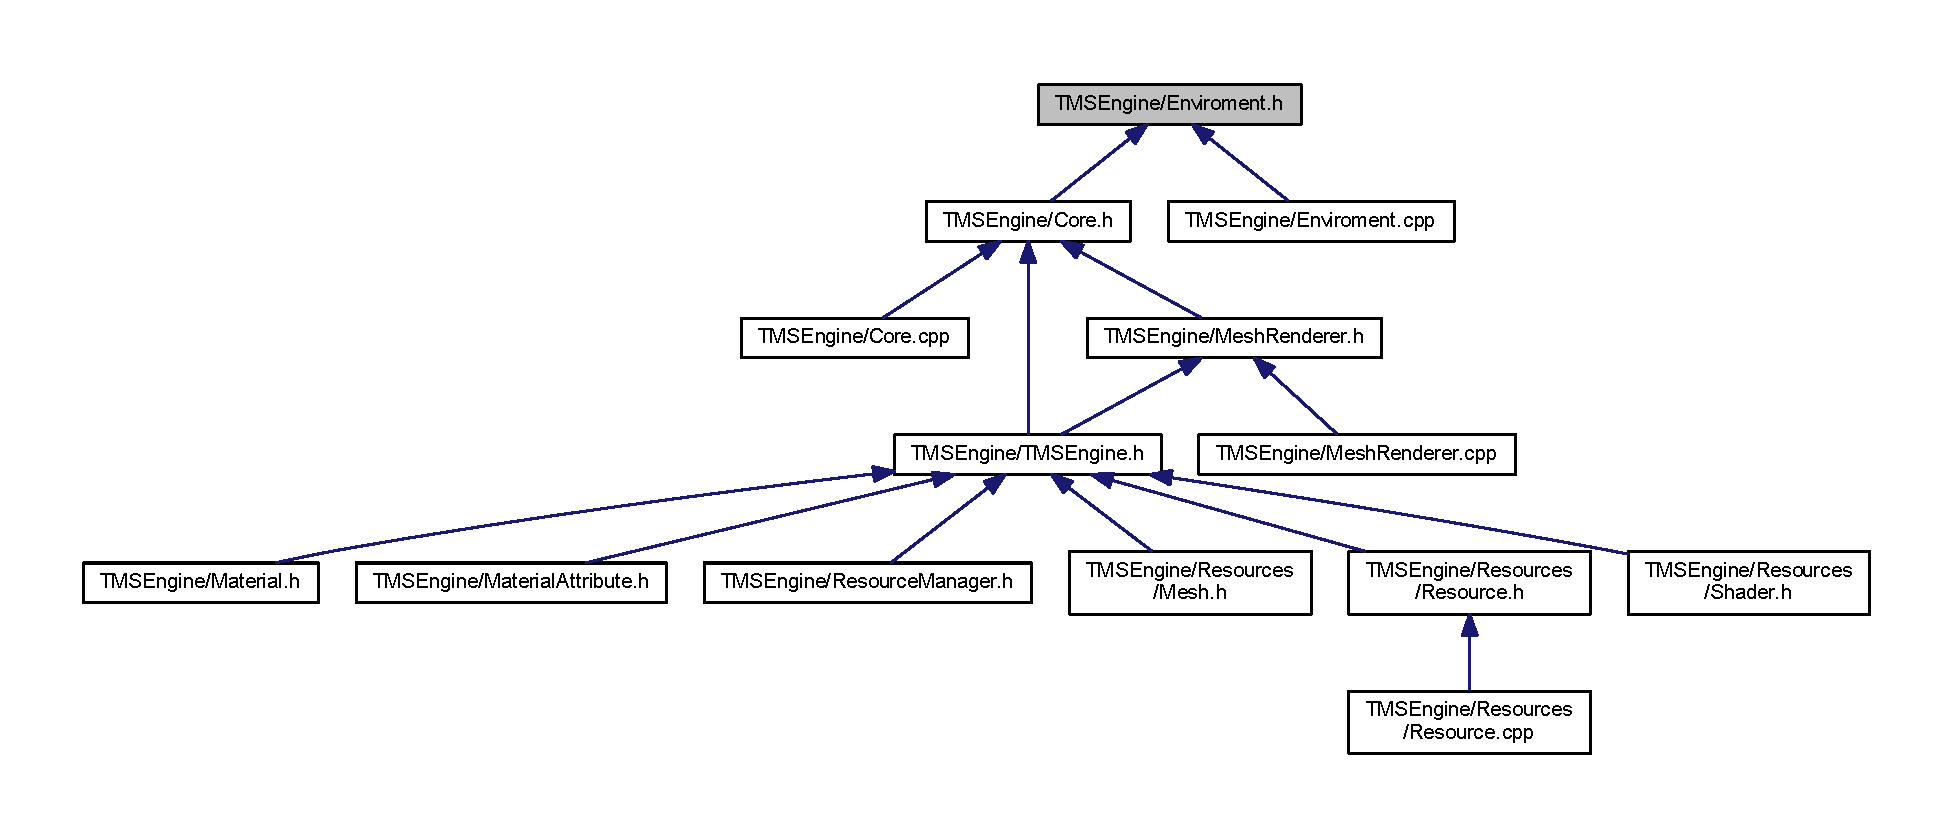
\includegraphics[width=350pt]{_enviroment_8h__dep__incl}
\end{center}
\end{figure}
\subsection*{Classes}
\begin{DoxyCompactItemize}
\item 
class \hyperlink{classtmsengine_1_1_enviroment}{tmsengine\+::\+Enviroment}
\end{DoxyCompactItemize}
\subsection*{Namespaces}
\begin{DoxyCompactItemize}
\item 
 \hyperlink{namespacetmsengine}{tmsengine}
\end{DoxyCompactItemize}

\hypertarget{_game_object_8cpp}{}\section{T\+M\+S\+Engine/\+Game\+Object.cpp File Reference}
\label{_game_object_8cpp}\index{T\+M\+S\+Engine/\+Game\+Object.\+cpp@{T\+M\+S\+Engine/\+Game\+Object.\+cpp}}
{\ttfamily \#include \char`\"{}Game\+Object.\+h\char`\"{}}\newline
Include dependency graph for Game\+Object.\+cpp\+:\nopagebreak
\begin{figure}[H]
\begin{center}
\leavevmode
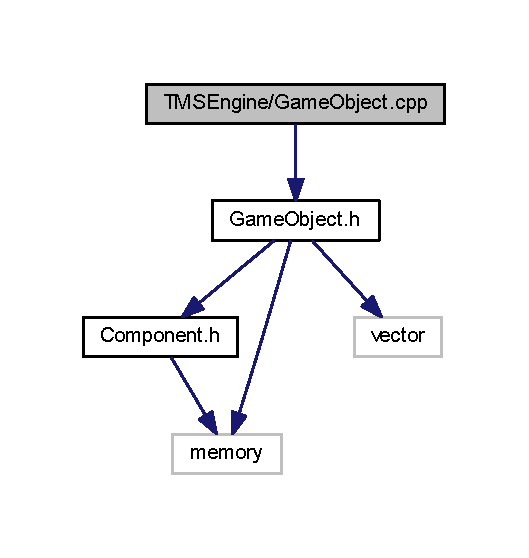
\includegraphics[width=254pt]{_game_object_8cpp__incl}
\end{center}
\end{figure}
\subsection*{Namespaces}
\begin{DoxyCompactItemize}
\item 
 \hyperlink{namespacetmsengine}{tmsengine}
\end{DoxyCompactItemize}

\hypertarget{_game_object_8h}{}\section{T\+M\+S\+Engine/\+Game\+Object.h File Reference}
\label{_game_object_8h}\index{T\+M\+S\+Engine/\+Game\+Object.\+h@{T\+M\+S\+Engine/\+Game\+Object.\+h}}
{\ttfamily \#include \char`\"{}Component.\+h\char`\"{}}\newline
{\ttfamily \#include $<$memory$>$}\newline
{\ttfamily \#include $<$vector$>$}\newline
Include dependency graph for Game\+Object.\+h\+:\nopagebreak
\begin{figure}[H]
\begin{center}
\leavevmode
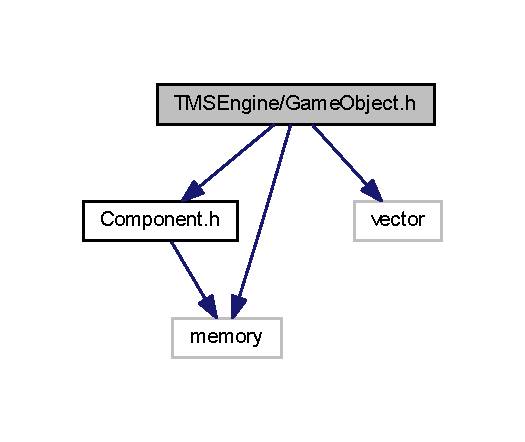
\includegraphics[width=252pt]{_game_object_8h__incl}
\end{center}
\end{figure}
This graph shows which files directly or indirectly include this file\+:
\nopagebreak
\begin{figure}[H]
\begin{center}
\leavevmode
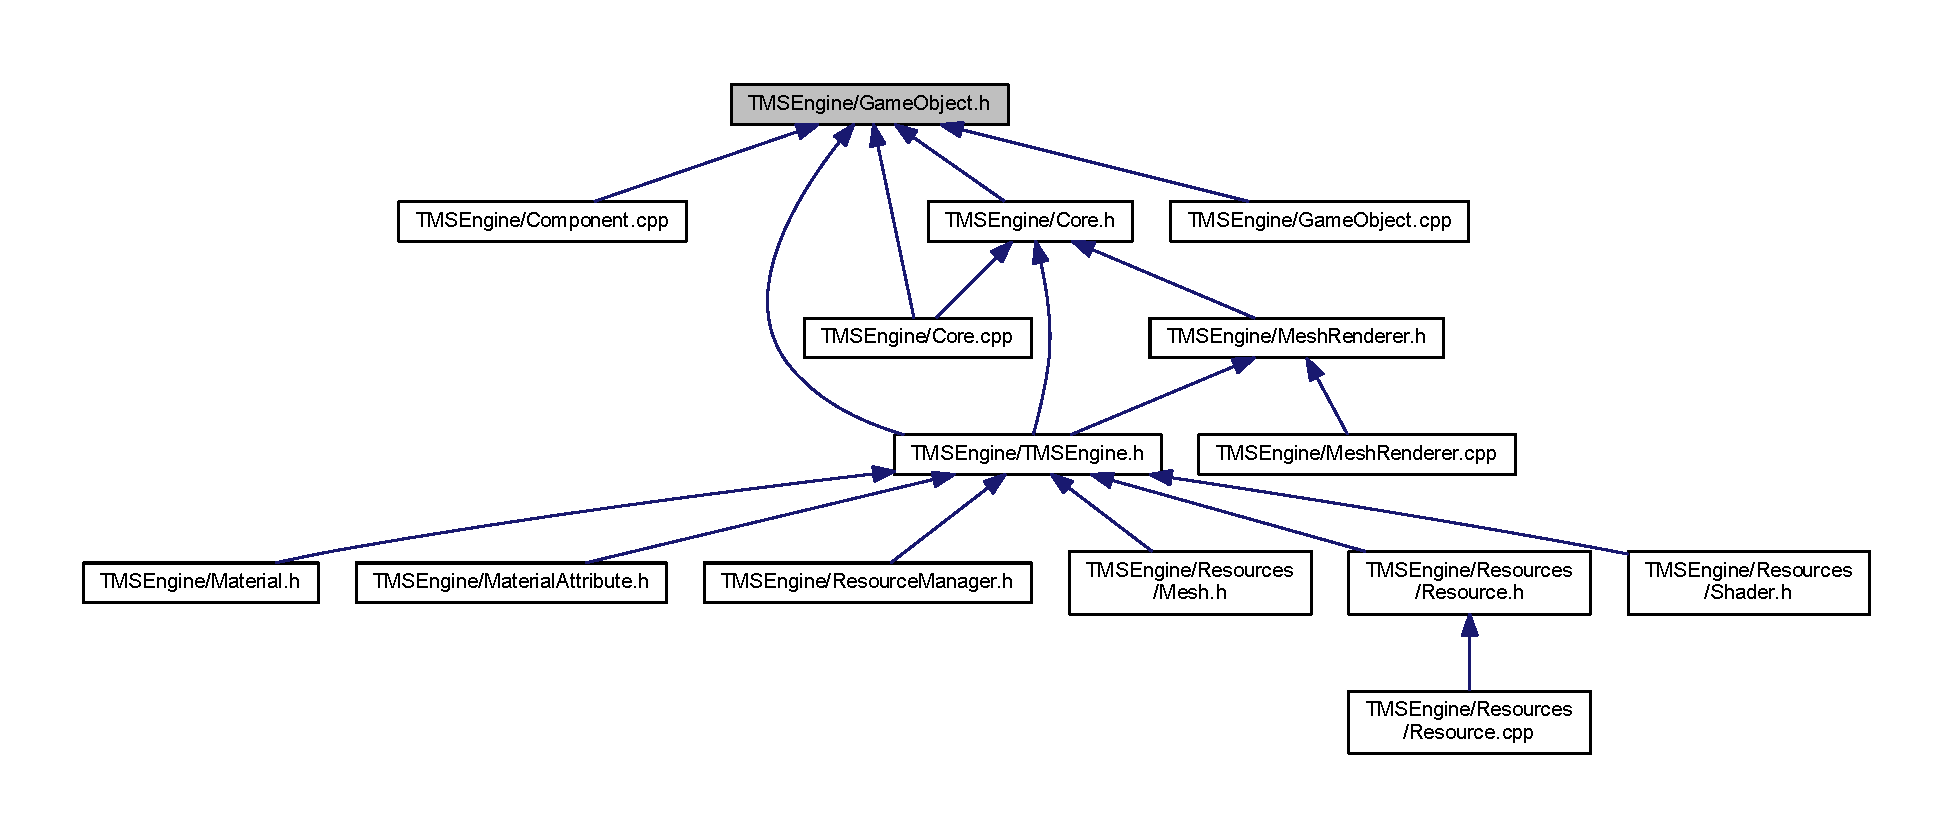
\includegraphics[width=350pt]{_game_object_8h__dep__incl}
\end{center}
\end{figure}
\subsection*{Classes}
\begin{DoxyCompactItemize}
\item 
class \hyperlink{classtmsengine_1_1_game_object}{tmsengine\+::\+Game\+Object}
\end{DoxyCompactItemize}
\subsection*{Namespaces}
\begin{DoxyCompactItemize}
\item 
 \hyperlink{namespacetmsengine}{tmsengine}
\end{DoxyCompactItemize}

\hypertarget{_keyboard_8cpp}{}\section{T\+M\+S\+Engine/\+Keyboard.cpp File Reference}
\label{_keyboard_8cpp}\index{T\+M\+S\+Engine/\+Keyboard.\+cpp@{T\+M\+S\+Engine/\+Keyboard.\+cpp}}
{\ttfamily \#include \char`\"{}Keyboard.\+h\char`\"{}}\newline
{\ttfamily \#include $<$iostream$>$}\newline
Include dependency graph for Keyboard.\+cpp\+:\nopagebreak
\begin{figure}[H]
\begin{center}
\leavevmode
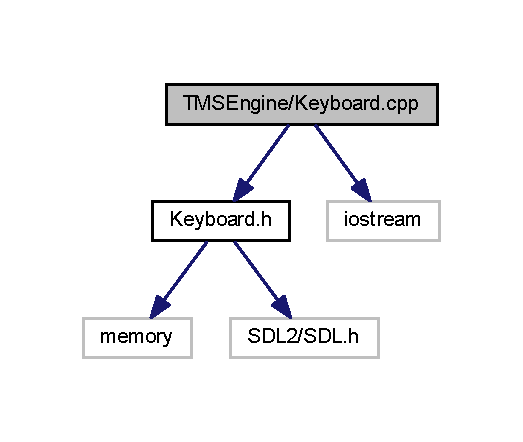
\includegraphics[width=251pt]{_keyboard_8cpp__incl}
\end{center}
\end{figure}
\subsection*{Namespaces}
\begin{DoxyCompactItemize}
\item 
 \hyperlink{namespacetmsengine}{tmsengine}
\end{DoxyCompactItemize}

\hypertarget{_keyboard_8h}{}\section{T\+M\+S\+Engine/\+Keyboard.h File Reference}
\label{_keyboard_8h}\index{T\+M\+S\+Engine/\+Keyboard.\+h@{T\+M\+S\+Engine/\+Keyboard.\+h}}
{\ttfamily \#include $<$memory$>$}\newline
{\ttfamily \#include \char`\"{}S\+D\+L2/\+S\+D\+L.\+h\char`\"{}}\newline
Include dependency graph for Keyboard.\+h\+:\nopagebreak
\begin{figure}[H]
\begin{center}
\leavevmode
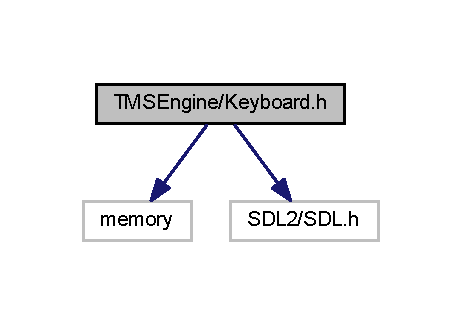
\includegraphics[width=222pt]{_keyboard_8h__incl}
\end{center}
\end{figure}
This graph shows which files directly or indirectly include this file\+:
\nopagebreak
\begin{figure}[H]
\begin{center}
\leavevmode
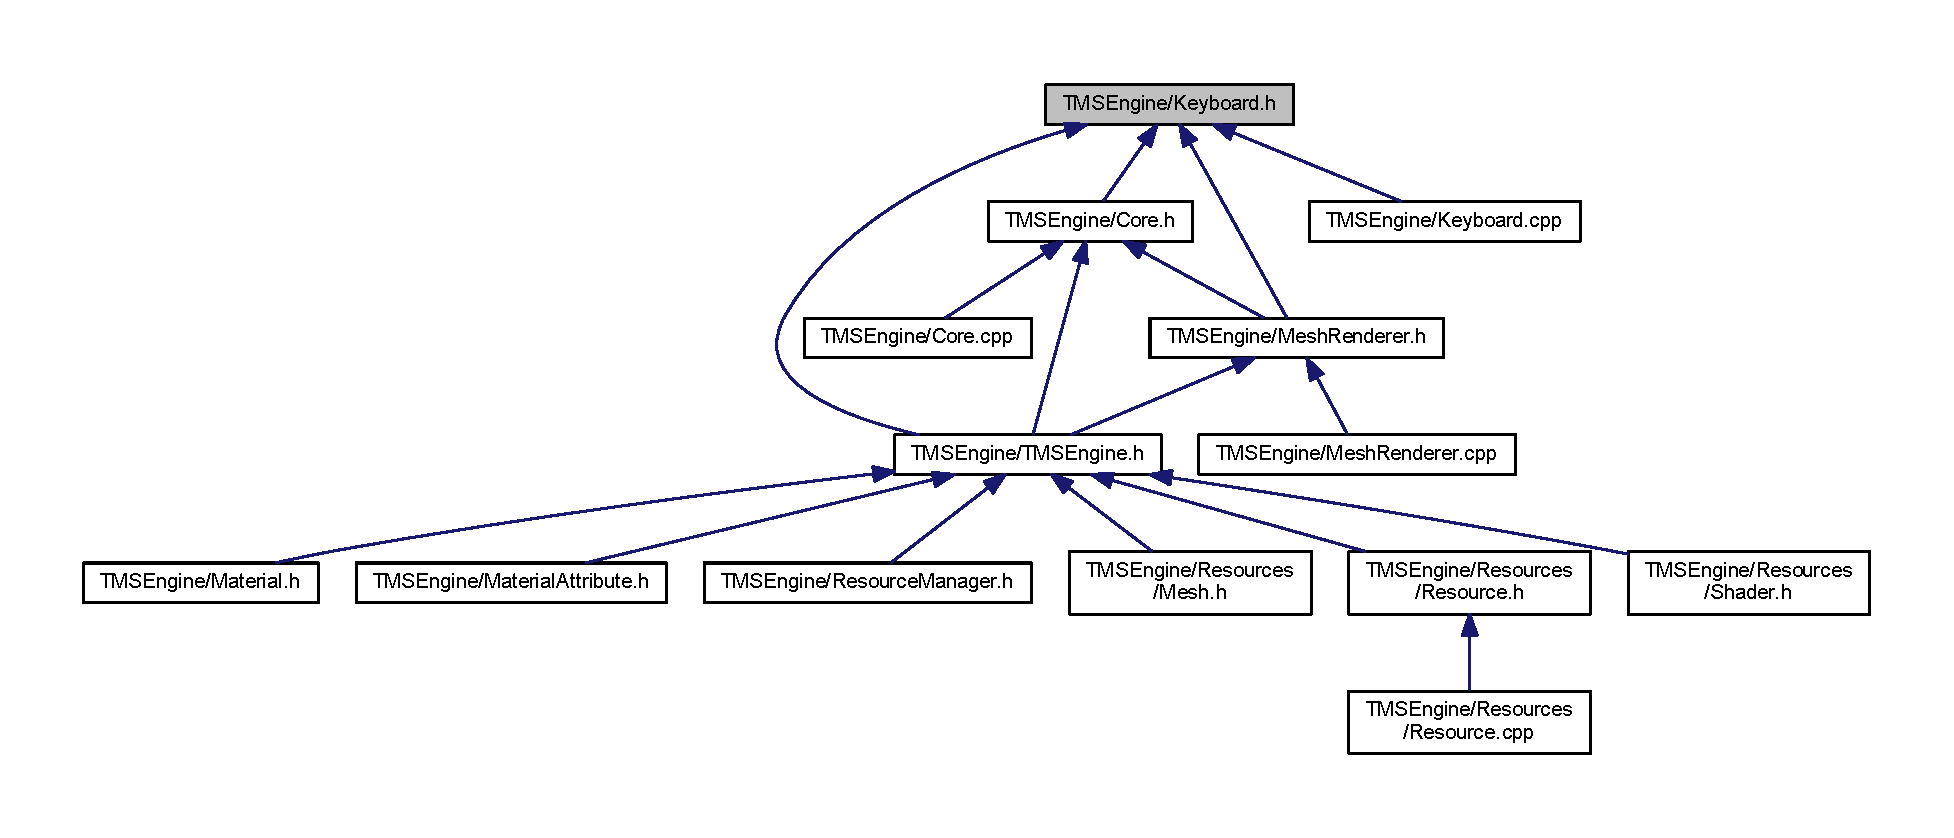
\includegraphics[width=350pt]{_keyboard_8h__dep__incl}
\end{center}
\end{figure}
\subsection*{Classes}
\begin{DoxyCompactItemize}
\item 
class \hyperlink{classtmsengine_1_1_keyboard}{tmsengine\+::\+Keyboard}
\end{DoxyCompactItemize}
\subsection*{Namespaces}
\begin{DoxyCompactItemize}
\item 
 \hyperlink{namespacetmsengine}{tmsengine}
\end{DoxyCompactItemize}

\hypertarget{_material_8cpp}{}\section{T\+M\+S\+Engine/\+Material.cpp File Reference}
\label{_material_8cpp}\index{T\+M\+S\+Engine/\+Material.\+cpp@{T\+M\+S\+Engine/\+Material.\+cpp}}

\hypertarget{_material_8h}{}\section{T\+M\+S\+Engine/\+Material.h File Reference}
\label{_material_8h}\index{T\+M\+S\+Engine/\+Material.\+h@{T\+M\+S\+Engine/\+Material.\+h}}
{\ttfamily \#include \char`\"{}T\+M\+S\+Engine/\+T\+M\+S\+Engine.\+h\char`\"{}}\newline
Include dependency graph for Material.\+h\+:
\nopagebreak
\begin{figure}[H]
\begin{center}
\leavevmode
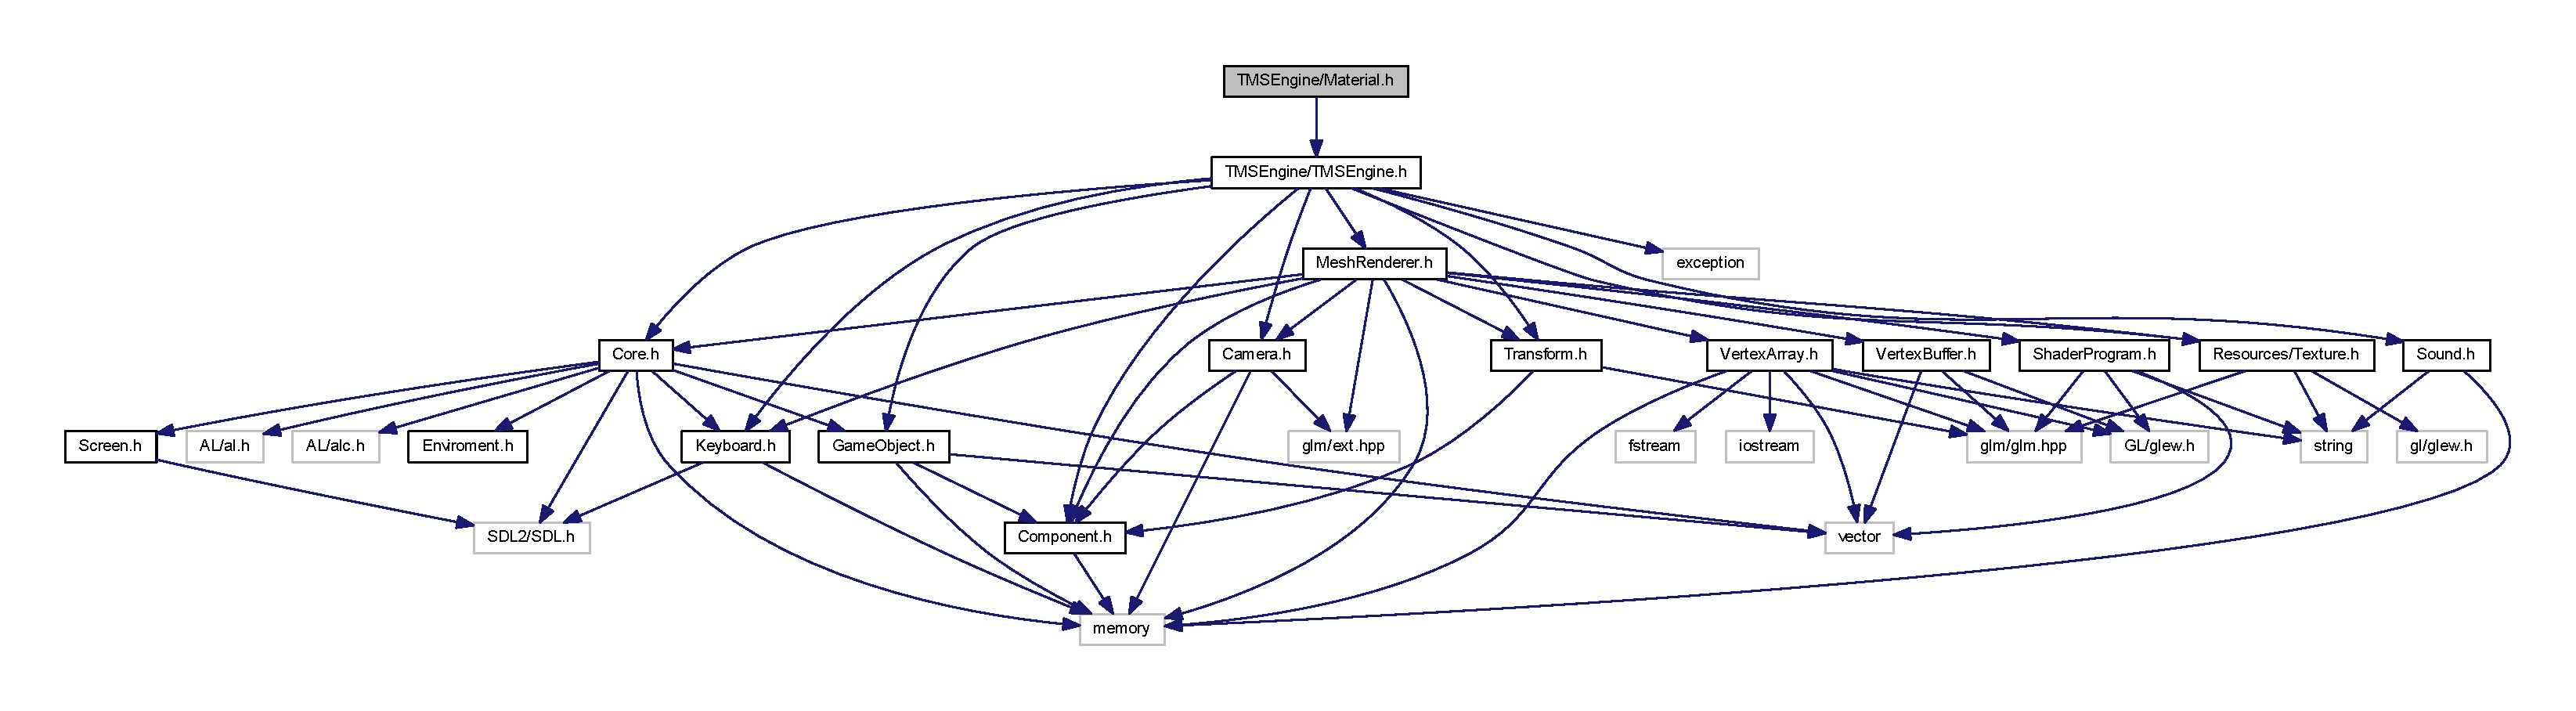
\includegraphics[width=350pt]{_material_8h__incl}
\end{center}
\end{figure}
\subsection*{Classes}
\begin{DoxyCompactItemize}
\item 
class \hyperlink{class_material}{Material}
\end{DoxyCompactItemize}

\hypertarget{_material_attribute_8cpp}{}\section{T\+M\+S\+Engine/\+Material\+Attribute.cpp File Reference}
\label{_material_attribute_8cpp}\index{T\+M\+S\+Engine/\+Material\+Attribute.\+cpp@{T\+M\+S\+Engine/\+Material\+Attribute.\+cpp}}

\hypertarget{_material_attribute_8h}{}\section{T\+M\+S\+Engine/\+Material\+Attribute.h File Reference}
\label{_material_attribute_8h}\index{T\+M\+S\+Engine/\+Material\+Attribute.\+h@{T\+M\+S\+Engine/\+Material\+Attribute.\+h}}
{\ttfamily \#include \char`\"{}T\+M\+S\+Engine/\+T\+M\+S\+Engine.\+h\char`\"{}}\newline
Include dependency graph for Material\+Attribute.\+h\+:
\nopagebreak
\begin{figure}[H]
\begin{center}
\leavevmode
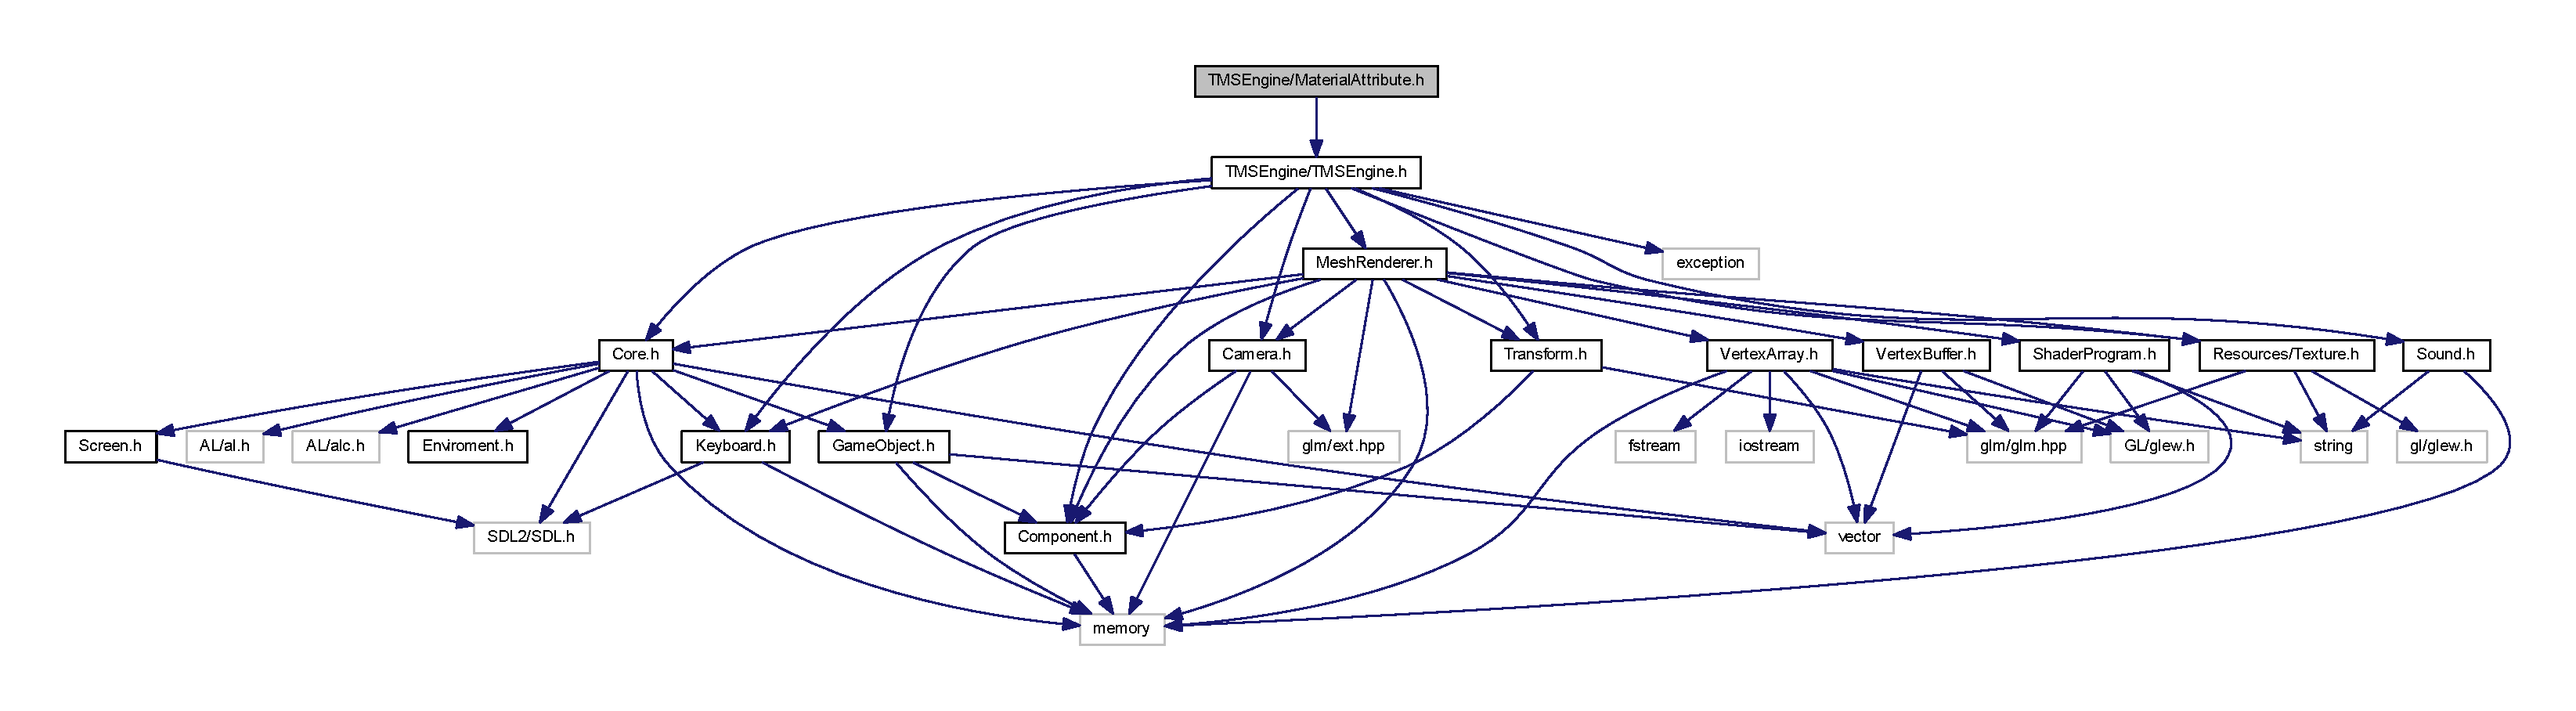
\includegraphics[width=350pt]{_material_attribute_8h__incl}
\end{center}
\end{figure}
\subsection*{Classes}
\begin{DoxyCompactItemize}
\item 
class \hyperlink{class_material_attribute}{Material\+Attribute}
\end{DoxyCompactItemize}

\hypertarget{_mesh_renderer_8cpp}{}\section{T\+M\+S\+Engine/\+Mesh\+Renderer.cpp File Reference}
\label{_mesh_renderer_8cpp}\index{T\+M\+S\+Engine/\+Mesh\+Renderer.\+cpp@{T\+M\+S\+Engine/\+Mesh\+Renderer.\+cpp}}
{\ttfamily \#include \char`\"{}Mesh\+Renderer.\+h\char`\"{}}\newline
{\ttfamily \#include $<$iostream$>$}\newline
{\ttfamily \#include $<$glm/ext.\+hpp$>$}\newline
Include dependency graph for Mesh\+Renderer.\+cpp\+:
\nopagebreak
\begin{figure}[H]
\begin{center}
\leavevmode
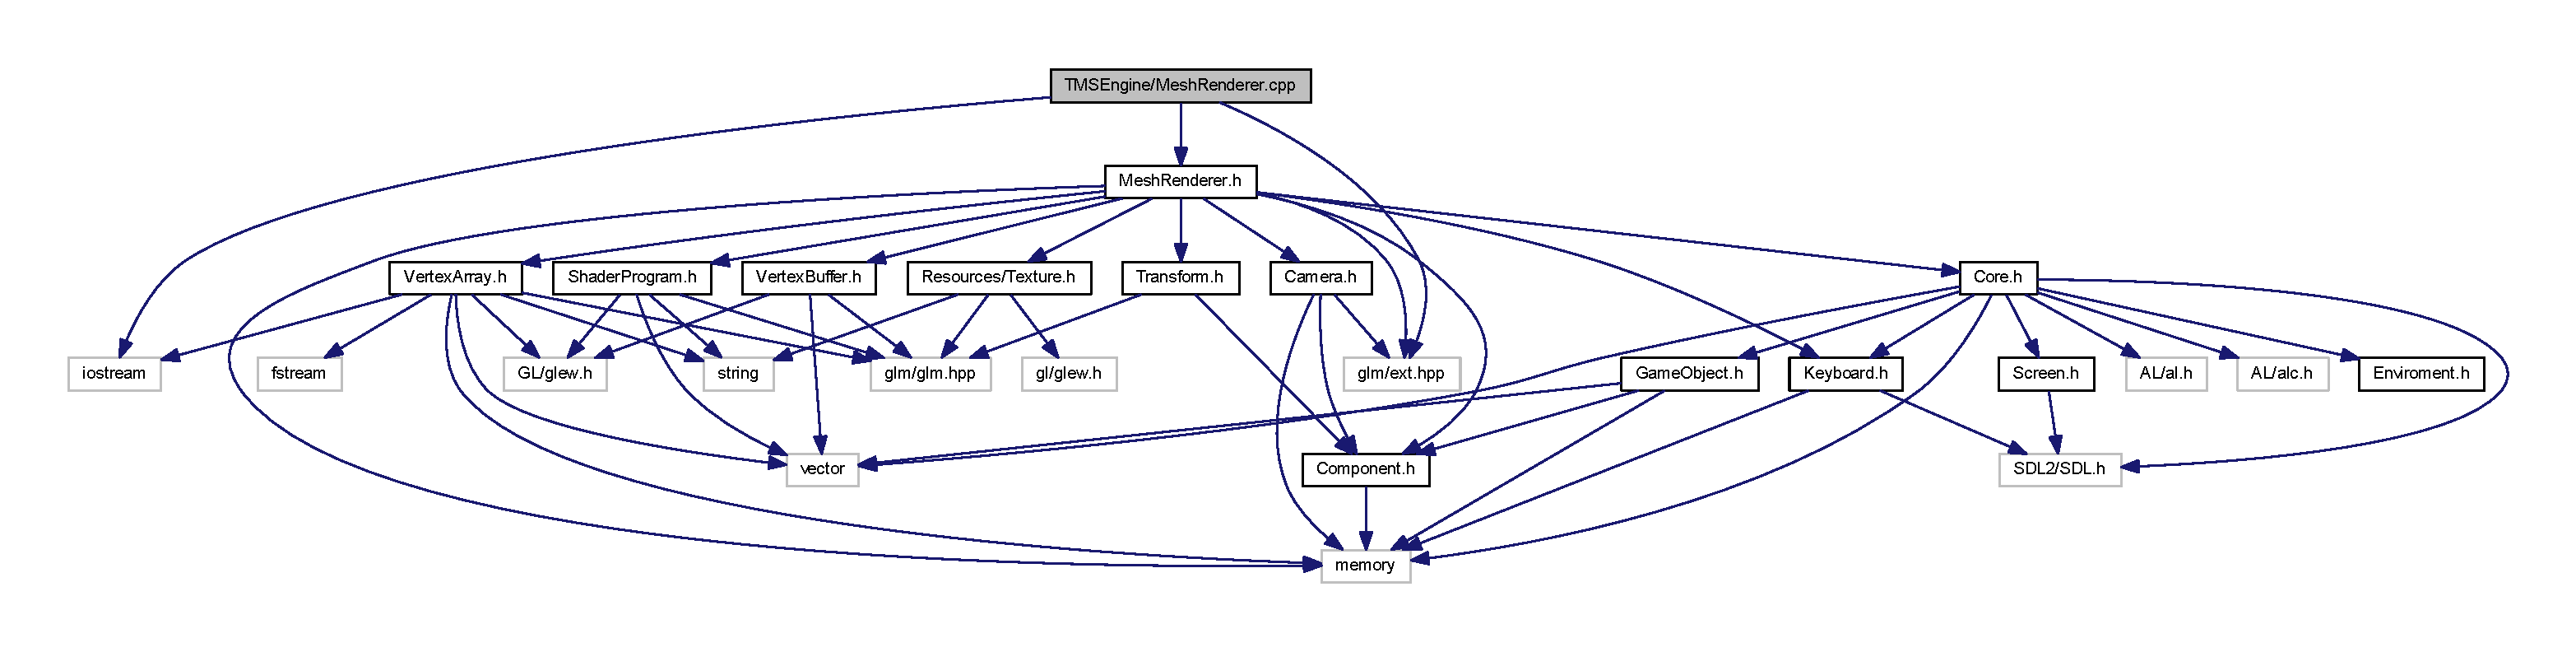
\includegraphics[width=350pt]{_mesh_renderer_8cpp__incl}
\end{center}
\end{figure}
\subsection*{Namespaces}
\begin{DoxyCompactItemize}
\item 
 \hyperlink{namespacetmsengine}{tmsengine}
\end{DoxyCompactItemize}

\hypertarget{_mesh_renderer_8h}{}\section{T\+M\+S\+Engine/\+Mesh\+Renderer.h File Reference}
\label{_mesh_renderer_8h}\index{T\+M\+S\+Engine/\+Mesh\+Renderer.\+h@{T\+M\+S\+Engine/\+Mesh\+Renderer.\+h}}
{\ttfamily \#include \char`\"{}Component.\+h\char`\"{}}\newline
{\ttfamily \#include $<$memory$>$}\newline
{\ttfamily \#include $<$glm/ext.\+hpp$>$}\newline
{\ttfamily \#include \char`\"{}Vertex\+Array.\+h\char`\"{}}\newline
{\ttfamily \#include \char`\"{}Vertex\+Buffer.\+h\char`\"{}}\newline
{\ttfamily \#include \char`\"{}Shader\+Program.\+h\char`\"{}}\newline
{\ttfamily \#include \char`\"{}Resources/\+Texture.\+h\char`\"{}}\newline
{\ttfamily \#include \char`\"{}Core.\+h\char`\"{}}\newline
{\ttfamily \#include \char`\"{}Camera.\+h\char`\"{}}\newline
{\ttfamily \#include \char`\"{}Transform.\+h\char`\"{}}\newline
{\ttfamily \#include \char`\"{}Keyboard.\+h\char`\"{}}\newline
Include dependency graph for Mesh\+Renderer.\+h\+:
\nopagebreak
\begin{figure}[H]
\begin{center}
\leavevmode
\includegraphics[width=350pt]{_mesh_renderer_8h__incl}
\end{center}
\end{figure}
This graph shows which files directly or indirectly include this file\+:
\nopagebreak
\begin{figure}[H]
\begin{center}
\leavevmode
\includegraphics[width=350pt]{_mesh_renderer_8h__dep__incl}
\end{center}
\end{figure}
\subsection*{Classes}
\begin{DoxyCompactItemize}
\item 
class \hyperlink{classtmsengine_1_1_mesh_renderer}{tmsengine\+::\+Mesh\+Renderer}
\end{DoxyCompactItemize}
\subsection*{Namespaces}
\begin{DoxyCompactItemize}
\item 
 \hyperlink{namespacetmsengine}{tmsengine}
\end{DoxyCompactItemize}

\hypertarget{_resource_manager_8cpp}{}\section{T\+M\+S\+Engine/\+Resource\+Manager.cpp File Reference}
\label{_resource_manager_8cpp}\index{T\+M\+S\+Engine/\+Resource\+Manager.\+cpp@{T\+M\+S\+Engine/\+Resource\+Manager.\+cpp}}

\hypertarget{_resource_manager_8h}{}\section{T\+M\+S\+Engine/\+Resource\+Manager.h File Reference}
\label{_resource_manager_8h}\index{T\+M\+S\+Engine/\+Resource\+Manager.\+h@{T\+M\+S\+Engine/\+Resource\+Manager.\+h}}
{\ttfamily \#include \char`\"{}T\+M\+S\+Engine/\+T\+M\+S\+Engine.\+h\char`\"{}}\newline
Include dependency graph for Resource\+Manager.\+h\+:
\nopagebreak
\begin{figure}[H]
\begin{center}
\leavevmode
\includegraphics[width=350pt]{_resource_manager_8h__incl}
\end{center}
\end{figure}
\subsection*{Classes}
\begin{DoxyCompactItemize}
\item 
class \hyperlink{class_resources}{Resources}
\end{DoxyCompactItemize}

\hypertarget{_mesh_8cpp}{}\section{T\+M\+S\+Engine/\+Resources/\+Mesh.cpp File Reference}
\label{_mesh_8cpp}\index{T\+M\+S\+Engine/\+Resources/\+Mesh.\+cpp@{T\+M\+S\+Engine/\+Resources/\+Mesh.\+cpp}}

\hypertarget{_mesh_8h}{}\section{T\+M\+S\+Engine/\+Resources/\+Mesh.h File Reference}
\label{_mesh_8h}\index{T\+M\+S\+Engine/\+Resources/\+Mesh.\+h@{T\+M\+S\+Engine/\+Resources/\+Mesh.\+h}}
{\ttfamily \#include \char`\"{}T\+M\+S\+Engine/\+T\+M\+S\+Engine.\+h\char`\"{}}\newline
Include dependency graph for Mesh.\+h\+:
\nopagebreak
\begin{figure}[H]
\begin{center}
\leavevmode
\includegraphics[width=350pt]{_mesh_8h__incl}
\end{center}
\end{figure}
\subsection*{Classes}
\begin{DoxyCompactItemize}
\item 
struct \hyperlink{struct_triangle}{Triangle}
\item 
class \hyperlink{class_mesh}{Mesh}
\end{DoxyCompactItemize}

\hypertarget{_resource_8cpp}{}\section{T\+M\+S\+Engine/\+Resources/\+Resource.cpp File Reference}
\label{_resource_8cpp}\index{T\+M\+S\+Engine/\+Resources/\+Resource.\+cpp@{T\+M\+S\+Engine/\+Resources/\+Resource.\+cpp}}
{\ttfamily \#include \char`\"{}Resource.\+h\char`\"{}}\newline
Include dependency graph for Resource.\+cpp\+:
\nopagebreak
\begin{figure}[H]
\begin{center}
\leavevmode
\includegraphics[width=350pt]{_resource_8cpp__incl}
\end{center}
\end{figure}

\hypertarget{_resource_8h}{}\section{T\+M\+S\+Engine/\+Resources/\+Resource.h File Reference}
\label{_resource_8h}\index{T\+M\+S\+Engine/\+Resources/\+Resource.\+h@{T\+M\+S\+Engine/\+Resources/\+Resource.\+h}}
{\ttfamily \#include \char`\"{}T\+M\+S\+Engine/\+T\+M\+S\+Engine.\+h\char`\"{}}\newline
Include dependency graph for Resource.\+h\+:
\nopagebreak
\begin{figure}[H]
\begin{center}
\leavevmode
\includegraphics[width=350pt]{_resource_8h__incl}
\end{center}
\end{figure}
This graph shows which files directly or indirectly include this file\+:\nopagebreak
\begin{figure}[H]
\begin{center}
\leavevmode
\includegraphics[width=196pt]{_resource_8h__dep__incl}
\end{center}
\end{figure}
\subsection*{Classes}
\begin{DoxyCompactItemize}
\item 
class \hyperlink{class_resource}{Resource}
\end{DoxyCompactItemize}

\hypertarget{_shader_8cpp}{}\section{T\+M\+S\+Engine/\+Resources/\+Shader.cpp File Reference}
\label{_shader_8cpp}\index{T\+M\+S\+Engine/\+Resources/\+Shader.\+cpp@{T\+M\+S\+Engine/\+Resources/\+Shader.\+cpp}}

\hypertarget{_shader_8h}{}\section{T\+M\+S\+Engine/\+Resources/\+Shader.h File Reference}
\label{_shader_8h}\index{T\+M\+S\+Engine/\+Resources/\+Shader.\+h@{T\+M\+S\+Engine/\+Resources/\+Shader.\+h}}
{\ttfamily \#include \char`\"{}T\+M\+S\+Engine/\+T\+M\+S\+Engine.\+h\char`\"{}}\newline
Include dependency graph for Shader.\+h\+:
\nopagebreak
\begin{figure}[H]
\begin{center}
\leavevmode
\includegraphics[width=350pt]{_shader_8h__incl}
\end{center}
\end{figure}
\subsection*{Classes}
\begin{DoxyCompactItemize}
\item 
class \hyperlink{class_shader}{Shader}
\end{DoxyCompactItemize}

\hypertarget{_texture_8cpp}{}\section{T\+M\+S\+Engine/\+Resources/\+Texture.cpp File Reference}
\label{_texture_8cpp}\index{T\+M\+S\+Engine/\+Resources/\+Texture.\+cpp@{T\+M\+S\+Engine/\+Resources/\+Texture.\+cpp}}
{\ttfamily \#include \char`\"{}Texture.\+h\char`\"{}}\newline
{\ttfamily \#include $<$stb\+\_\+image/stb\+\_\+image.\+h$>$}\newline
Include dependency graph for Texture.\+cpp\+:\nopagebreak
\begin{figure}[H]
\begin{center}
\leavevmode
\includegraphics[width=350pt]{_texture_8cpp__incl}
\end{center}
\end{figure}
\subsection*{Namespaces}
\begin{DoxyCompactItemize}
\item 
 \hyperlink{namespacetmsengine}{tmsengine}
\end{DoxyCompactItemize}

\hypertarget{_texture_8h}{}\section{T\+M\+S\+Engine/\+Resources/\+Texture.h File Reference}
\label{_texture_8h}\index{T\+M\+S\+Engine/\+Resources/\+Texture.\+h@{T\+M\+S\+Engine/\+Resources/\+Texture.\+h}}
{\ttfamily \#include $<$gl/glew.\+h$>$}\newline
{\ttfamily \#include $<$glm/glm.\+hpp$>$}\newline
{\ttfamily \#include $<$string$>$}\newline
Include dependency graph for Texture.\+h\+:\nopagebreak
\begin{figure}[H]
\begin{center}
\leavevmode
\includegraphics[width=283pt]{_texture_8h__incl}
\end{center}
\end{figure}
This graph shows which files directly or indirectly include this file\+:
\nopagebreak
\begin{figure}[H]
\begin{center}
\leavevmode
\includegraphics[width=350pt]{_texture_8h__dep__incl}
\end{center}
\end{figure}
\subsection*{Classes}
\begin{DoxyCompactItemize}
\item 
class \hyperlink{classtmsengine_1_1_texture}{tmsengine\+::\+Texture}
\end{DoxyCompactItemize}
\subsection*{Namespaces}
\begin{DoxyCompactItemize}
\item 
 \hyperlink{namespacetmsengine}{tmsengine}
\end{DoxyCompactItemize}

\hypertarget{_screen_8cpp}{}\section{T\+M\+S\+Engine/\+Screen.cpp File Reference}
\label{_screen_8cpp}\index{T\+M\+S\+Engine/\+Screen.\+cpp@{T\+M\+S\+Engine/\+Screen.\+cpp}}
{\ttfamily \#include \char`\"{}Screen.\+h\char`\"{}}\newline
{\ttfamily \#include $<$G\+L/glew.\+h$>$}\newline
{\ttfamily \#include $<$iostream$>$}\newline
{\ttfamily \#include $<$string$>$}\newline
Include dependency graph for Screen.\+cpp\+:\nopagebreak
\begin{figure}[H]
\begin{center}
\leavevmode
\includegraphics[width=350pt]{_screen_8cpp__incl}
\end{center}
\end{figure}
\subsection*{Namespaces}
\begin{DoxyCompactItemize}
\item 
 \hyperlink{namespacetmsengine}{tmsengine}
\end{DoxyCompactItemize}

\hypertarget{_screen_8h}{}\section{T\+M\+S\+Engine/\+Screen.h File Reference}
\label{_screen_8h}\index{T\+M\+S\+Engine/\+Screen.\+h@{T\+M\+S\+Engine/\+Screen.\+h}}
{\ttfamily \#include $<$S\+D\+L2/\+S\+D\+L.\+h$>$}\newline
Include dependency graph for Screen.\+h\+:\nopagebreak
\begin{figure}[H]
\begin{center}
\leavevmode
\includegraphics[width=189pt]{_screen_8h__incl}
\end{center}
\end{figure}
This graph shows which files directly or indirectly include this file\+:
\nopagebreak
\begin{figure}[H]
\begin{center}
\leavevmode
\includegraphics[width=350pt]{_screen_8h__dep__incl}
\end{center}
\end{figure}
\subsection*{Classes}
\begin{DoxyCompactItemize}
\item 
class \hyperlink{classtmsengine_1_1_screen}{tmsengine\+::\+Screen}
\end{DoxyCompactItemize}
\subsection*{Namespaces}
\begin{DoxyCompactItemize}
\item 
 \hyperlink{namespacetmsengine}{tmsengine}
\end{DoxyCompactItemize}

\hypertarget{_shader_program_8cpp}{}\section{T\+M\+S\+Engine/\+Shader\+Program.cpp File Reference}
\label{_shader_program_8cpp}\index{T\+M\+S\+Engine/\+Shader\+Program.\+cpp@{T\+M\+S\+Engine/\+Shader\+Program.\+cpp}}
{\ttfamily \#include \char`\"{}Shader\+Program.\+h\char`\"{}}\newline
{\ttfamily \#include \char`\"{}Vertex\+Array.\+h\char`\"{}}\newline
{\ttfamily \#include \char`\"{}Resources/\+Texture.\+h\char`\"{}}\newline
{\ttfamily \#include $<$glm/ext.\+hpp$>$}\newline
{\ttfamily \#include $<$fstream$>$}\newline
{\ttfamily \#include $<$iostream$>$}\newline
Include dependency graph for Shader\+Program.\+cpp\+:\nopagebreak
\begin{figure}[H]
\begin{center}
\leavevmode
\includegraphics[width=350pt]{_shader_program_8cpp__incl}
\end{center}
\end{figure}

\hypertarget{_shader_program_8h}{}\section{T\+M\+S\+Engine/\+Shader\+Program.h File Reference}
\label{_shader_program_8h}\index{T\+M\+S\+Engine/\+Shader\+Program.\+h@{T\+M\+S\+Engine/\+Shader\+Program.\+h}}
{\ttfamily \#include $<$G\+L/glew.\+h$>$}\newline
{\ttfamily \#include $<$glm/glm.\+hpp$>$}\newline
{\ttfamily \#include $<$string$>$}\newline
{\ttfamily \#include $<$vector$>$}\newline
Include dependency graph for Shader\+Program.\+h\+:\nopagebreak
\begin{figure}[H]
\begin{center}
\leavevmode
\includegraphics[width=348pt]{_shader_program_8h__incl}
\end{center}
\end{figure}
This graph shows which files directly or indirectly include this file\+:
\nopagebreak
\begin{figure}[H]
\begin{center}
\leavevmode
\includegraphics[width=350pt]{_shader_program_8h__dep__incl}
\end{center}
\end{figure}
\subsection*{Classes}
\begin{DoxyCompactItemize}
\item 
struct \hyperlink{structtmsengine_1_1_sampler}{tmsengine\+::\+Sampler}
\item 
class \hyperlink{classtmsengine_1_1_shader_program}{tmsengine\+::\+Shader\+Program}
\end{DoxyCompactItemize}
\subsection*{Namespaces}
\begin{DoxyCompactItemize}
\item 
 \hyperlink{namespacetmsengine}{tmsengine}
\end{DoxyCompactItemize}

\hypertarget{_sound_8cpp}{}\section{T\+M\+S\+Engine/\+Sound.cpp File Reference}
\label{_sound_8cpp}\index{T\+M\+S\+Engine/\+Sound.\+cpp@{T\+M\+S\+Engine/\+Sound.\+cpp}}
{\ttfamily \#include \char`\"{}Sound.\+h\char`\"{}}\newline
{\ttfamily \#include $<$A\+L/al.\+h$>$}\newline
{\ttfamily \#include $<$vorbis/vorbisfile.\+h$>$}\newline
{\ttfamily \#include $<$iostream$>$}\newline
{\ttfamily \#include $<$vector$>$}\newline
Include dependency graph for Sound.\+cpp\+:\nopagebreak
\begin{figure}[H]
\begin{center}
\leavevmode
\includegraphics[width=350pt]{_sound_8cpp__incl}
\end{center}
\end{figure}
\subsection*{Classes}
\begin{DoxyCompactItemize}
\item 
struct \hyperlink{structtmsengine_1_1_sound_impl}{tmsengine\+::\+Sound\+Impl}
\end{DoxyCompactItemize}
\subsection*{Namespaces}
\begin{DoxyCompactItemize}
\item 
 \hyperlink{namespacetmsengine}{tmsengine}
\end{DoxyCompactItemize}

\hypertarget{_sound_8h}{}\section{T\+M\+S\+Engine/\+Sound.h File Reference}
\label{_sound_8h}\index{T\+M\+S\+Engine/\+Sound.\+h@{T\+M\+S\+Engine/\+Sound.\+h}}
{\ttfamily \#include $<$memory$>$}\newline
{\ttfamily \#include $<$string$>$}\newline
Include dependency graph for Sound.\+h\+:\nopagebreak
\begin{figure}[H]
\begin{center}
\leavevmode
\includegraphics[width=192pt]{_sound_8h__incl}
\end{center}
\end{figure}
This graph shows which files directly or indirectly include this file\+:
\nopagebreak
\begin{figure}[H]
\begin{center}
\leavevmode
\includegraphics[width=350pt]{_sound_8h__dep__incl}
\end{center}
\end{figure}
\subsection*{Classes}
\begin{DoxyCompactItemize}
\item 
class \hyperlink{classtmsengine_1_1_sound}{tmsengine\+::\+Sound}
\end{DoxyCompactItemize}
\subsection*{Namespaces}
\begin{DoxyCompactItemize}
\item 
 \hyperlink{namespacetmsengine}{tmsengine}
\end{DoxyCompactItemize}

\hypertarget{_t_m_s_engine_8h}{}\section{T\+M\+S\+Engine/\+T\+M\+S\+Engine.h File Reference}
\label{_t_m_s_engine_8h}\index{T\+M\+S\+Engine/\+T\+M\+S\+Engine.\+h@{T\+M\+S\+Engine/\+T\+M\+S\+Engine.\+h}}
{\ttfamily \#include \char`\"{}Core.\+h\char`\"{}}\newline
{\ttfamily \#include \char`\"{}Game\+Object.\+h\char`\"{}}\newline
{\ttfamily \#include \char`\"{}Component.\+h\char`\"{}}\newline
{\ttfamily \#include \char`\"{}Mesh\+Renderer.\+h\char`\"{}}\newline
{\ttfamily \#include \char`\"{}Sound.\+h\char`\"{}}\newline
{\ttfamily \#include \char`\"{}Transform.\+h\char`\"{}}\newline
{\ttfamily \#include \char`\"{}Camera.\+h\char`\"{}}\newline
{\ttfamily \#include \char`\"{}Resources/\+Texture.\+h\char`\"{}}\newline
{\ttfamily \#include \char`\"{}Keyboard.\+h\char`\"{}}\newline
{\ttfamily \#include $<$exception$>$}\newline
Include dependency graph for T\+M\+S\+Engine.\+h\+:
\nopagebreak
\begin{figure}[H]
\begin{center}
\leavevmode
\includegraphics[width=350pt]{_t_m_s_engine_8h__incl}
\end{center}
\end{figure}
This graph shows which files directly or indirectly include this file\+:
\nopagebreak
\begin{figure}[H]
\begin{center}
\leavevmode
\includegraphics[width=350pt]{_t_m_s_engine_8h__dep__incl}
\end{center}
\end{figure}
\subsection*{Macros}
\begin{DoxyCompactItemize}
\item 
\#define \hyperlink{_t_m_s_engine_8h_ae24e9d338c310db25ac9945686a611f5}{T\+M\+S\+E\+N\+G\+I\+N\+E\+\_\+\+H\+\_\+}
\end{DoxyCompactItemize}


\subsection{Macro Definition Documentation}
\mbox{\Hypertarget{_t_m_s_engine_8h_ae24e9d338c310db25ac9945686a611f5}\label{_t_m_s_engine_8h_ae24e9d338c310db25ac9945686a611f5}} 
\index{T\+M\+S\+Engine.\+h@{T\+M\+S\+Engine.\+h}!T\+M\+S\+E\+N\+G\+I\+N\+E\+\_\+\+H\+\_\+@{T\+M\+S\+E\+N\+G\+I\+N\+E\+\_\+\+H\+\_\+}}
\index{T\+M\+S\+E\+N\+G\+I\+N\+E\+\_\+\+H\+\_\+@{T\+M\+S\+E\+N\+G\+I\+N\+E\+\_\+\+H\+\_\+}!T\+M\+S\+Engine.\+h@{T\+M\+S\+Engine.\+h}}
\subsubsection{\texorpdfstring{T\+M\+S\+E\+N\+G\+I\+N\+E\+\_\+\+H\+\_\+}{TMSENGINE\_H\_}}
{\footnotesize\ttfamily \#define T\+M\+S\+E\+N\+G\+I\+N\+E\+\_\+\+H\+\_\+}


\hypertarget{_transform_8cpp}{}\section{T\+M\+S\+Engine/\+Transform.cpp File Reference}
\label{_transform_8cpp}\index{T\+M\+S\+Engine/\+Transform.\+cpp@{T\+M\+S\+Engine/\+Transform.\+cpp}}
{\ttfamily \#include \char`\"{}Transform.\+h\char`\"{}}\newline
Include dependency graph for Transform.\+cpp\+:
\nopagebreak
\begin{figure}[H]
\begin{center}
\leavevmode
\includegraphics[width=242pt]{_transform_8cpp__incl}
\end{center}
\end{figure}
\subsection*{Namespaces}
\begin{DoxyCompactItemize}
\item 
 \hyperlink{namespacetmsengine}{tmsengine}
\end{DoxyCompactItemize}

\hypertarget{_transform_8h}{}\section{T\+M\+S\+Engine/\+Transform.h File Reference}
\label{_transform_8h}\index{T\+M\+S\+Engine/\+Transform.\+h@{T\+M\+S\+Engine/\+Transform.\+h}}
{\ttfamily \#include $<$glm/glm.\+hpp$>$}\newline
{\ttfamily \#include \char`\"{}Component.\+h\char`\"{}}\newline
Include dependency graph for Transform.\+h\+:
\nopagebreak
\begin{figure}[H]
\begin{center}
\leavevmode
\includegraphics[width=242pt]{_transform_8h__incl}
\end{center}
\end{figure}
This graph shows which files directly or indirectly include this file\+:
\nopagebreak
\begin{figure}[H]
\begin{center}
\leavevmode
\includegraphics[width=350pt]{_transform_8h__dep__incl}
\end{center}
\end{figure}
\subsection*{Classes}
\begin{DoxyCompactItemize}
\item 
class \hyperlink{classtmsengine_1_1_transform}{tmsengine\+::\+Transform}
\end{DoxyCompactItemize}
\subsection*{Namespaces}
\begin{DoxyCompactItemize}
\item 
 \hyperlink{namespacetmsengine}{tmsengine}
\end{DoxyCompactItemize}

\hypertarget{_vertex_array_8cpp}{}\section{T\+M\+S\+Engine/\+Vertex\+Array.cpp File Reference}
\label{_vertex_array_8cpp}\index{T\+M\+S\+Engine/\+Vertex\+Array.\+cpp@{T\+M\+S\+Engine/\+Vertex\+Array.\+cpp}}
{\ttfamily \#include \char`\"{}Vertex\+Array.\+h\char`\"{}}\newline
{\ttfamily \#include \char`\"{}Vertex\+Buffer.\+h\char`\"{}}\newline
{\ttfamily \#include $<$fstream$>$}\newline
{\ttfamily \#include $<$iostream$>$}\newline
Include dependency graph for Vertex\+Array.\+cpp\+:\nopagebreak
\begin{figure}[H]
\begin{center}
\leavevmode
\includegraphics[width=350pt]{_vertex_array_8cpp__incl}
\end{center}
\end{figure}

\hypertarget{_vertex_array_8h}{}\section{T\+M\+S\+Engine/\+Vertex\+Array.h File Reference}
\label{_vertex_array_8h}\index{T\+M\+S\+Engine/\+Vertex\+Array.\+h@{T\+M\+S\+Engine/\+Vertex\+Array.\+h}}
{\ttfamily \#include $<$G\+L/glew.\+h$>$}\newline
{\ttfamily \#include $<$glm/glm.\+hpp$>$}\newline
{\ttfamily \#include $<$vector$>$}\newline
{\ttfamily \#include $<$string$>$}\newline
{\ttfamily \#include $<$memory$>$}\newline
{\ttfamily \#include $<$fstream$>$}\newline
{\ttfamily \#include $<$iostream$>$}\newline
Include dependency graph for Vertex\+Array.\+h\+:\nopagebreak
\begin{figure}[H]
\begin{center}
\leavevmode
\includegraphics[width=350pt]{_vertex_array_8h__incl}
\end{center}
\end{figure}
This graph shows which files directly or indirectly include this file\+:
\nopagebreak
\begin{figure}[H]
\begin{center}
\leavevmode
\includegraphics[width=350pt]{_vertex_array_8h__dep__incl}
\end{center}
\end{figure}
\subsection*{Classes}
\begin{DoxyCompactItemize}
\item 
class \hyperlink{classtmsengine_1_1_vertex_array}{tmsengine\+::\+Vertex\+Array}
\end{DoxyCompactItemize}
\subsection*{Namespaces}
\begin{DoxyCompactItemize}
\item 
 \hyperlink{namespacetmsengine}{tmsengine}
\end{DoxyCompactItemize}

\hypertarget{_vertex_buffer_8cpp}{}\section{T\+M\+S\+Engine/\+Vertex\+Buffer.cpp File Reference}
\label{_vertex_buffer_8cpp}\index{T\+M\+S\+Engine/\+Vertex\+Buffer.\+cpp@{T\+M\+S\+Engine/\+Vertex\+Buffer.\+cpp}}
{\ttfamily \#include \char`\"{}Vertex\+Buffer.\+h\char`\"{}}\newline
{\ttfamily \#include $<$iostream$>$}\newline
Include dependency graph for Vertex\+Buffer.\+cpp\+:\nopagebreak
\begin{figure}[H]
\begin{center}
\leavevmode
\includegraphics[width=306pt]{_vertex_buffer_8cpp__incl}
\end{center}
\end{figure}

\hypertarget{_vertex_buffer_8h}{}\section{T\+M\+S\+Engine/\+Vertex\+Buffer.h File Reference}
\label{_vertex_buffer_8h}\index{T\+M\+S\+Engine/\+Vertex\+Buffer.\+h@{T\+M\+S\+Engine/\+Vertex\+Buffer.\+h}}
{\ttfamily \#include $<$G\+L/glew.\+h$>$}\newline
{\ttfamily \#include $<$glm/glm.\+hpp$>$}\newline
{\ttfamily \#include $<$vector$>$}\newline
Include dependency graph for Vertex\+Buffer.\+h\+:\nopagebreak
\begin{figure}[H]
\begin{center}
\leavevmode
\includegraphics[width=288pt]{_vertex_buffer_8h__incl}
\end{center}
\end{figure}
This graph shows which files directly or indirectly include this file\+:
\nopagebreak
\begin{figure}[H]
\begin{center}
\leavevmode
\includegraphics[width=350pt]{_vertex_buffer_8h__dep__incl}
\end{center}
\end{figure}
\subsection*{Classes}
\begin{DoxyCompactItemize}
\item 
class \hyperlink{classtmsengine_1_1_vertex_buffer}{tmsengine\+::\+Vertex\+Buffer}
\end{DoxyCompactItemize}
\subsection*{Namespaces}
\begin{DoxyCompactItemize}
\item 
 \hyperlink{namespacetmsengine}{tmsengine}
\end{DoxyCompactItemize}

%--- End generated contents ---

% Index
\backmatter
\newpage
\phantomsection
\clearemptydoublepage
\addcontentsline{toc}{chapter}{Index}
\printindex

\end{document}
